\documentclass[12pt,a4paper]{article}

% ============================================================
%                   CẤU HÌNH GÓI LỆNH (PREAMBLE)
% ============================================================
\usepackage[utf8]{inputenc}
\usepackage[T5]{fontenc}
\usepackage[vietnamese]{babel}
\usepackage{amsmath}
\usepackage{amssymb}
\usepackage{geometry}
\geometry{a4paper, left=3cm, right=2cm, top=2.5cm, bottom=2.5cm, headheight=15pt}

% Đồ họa & Đường dẫn hình ảnh dùng chung
\usepackage{graphicx}
\graphicspath{{../assets/}{../../diagrams/}{./}}

% Bảng biểu nâng cao & Định dạng
\usepackage{booktabs}
\usepackage{longtable}
\usepackage{tabularx}
\usepackage{array}
\usepackage{multirow}
\usepackage{float}
\usepackage{xcolor}
\usepackage{enumitem}
\usepackage{indentfirst}

% Khung viền trang bìa & Đồ họa TikZ
\usepackage{tikz}
\usetikzlibrary{calc, shapes.geometric, arrows.meta, positioning, shadows}

% Định dạng tiêu đề các mục (Mục 1, Mục 2, ...)
\usepackage{titlesec}
\titleformat{\section}[hang]{\normalfont\LARGE\bfseries}{\textbf{Mục \thesection:}}{0.5em}{}
\titlespacing*{\section}{0pt}{24pt}{12pt}
\titleformat{\subsection}[hang]{\normalfont\Large\bfseries}{\thesubsection}{0.6em}{}
\titlespacing*{\subsection}{0pt}{16pt}{8pt}
\titleformat{\subsubsection}[hang]{\normalfont\large\bfseries}{\thesubsubsection}{0.6em}{}
\titlespacing*{\subsubsection}{0pt}{12pt}{6pt}

% Header & Footer chuẩn trường ĐH Bách Khoa
\usepackage{fancyhdr}
\pagestyle{fancy}
\fancyhf{}
\fancyhead[L]{\small CO3001 -- Công nghệ Phần mềm HK261}
\fancyhead[R]{\small Nhóm BEE BRAVE}
\fancyfoot[C]{\thepage}
\renewcommand{\headrulewidth}{0.4pt}

\fancypagestyle{plain}{
  \fancyhf{}
  \fancyhead[L]{\small CO3001 -- Công nghệ Phần mềm HK261}
  \fancyhead[R]{\small Nhóm BEE BRAVE}
  \fancyfoot[C]{\thepage}
  \renewcommand{\headrulewidth}{0.4pt}
}

% Hyperlink & Metadata
\usepackage{hyperref}
\hypersetup{
    colorlinks=true,
    linkcolor=blue,
    filecolor=magenta,
    urlcolor=blue,
    pdftitle={Smart E-Mobility Hub -- Báo cáo Thiết kế Kiến trúc và Chi tiết Hệ thống (Submission 2)},
    pdfauthor={Nhóm BEE BRAVE -- L02},
}

\begin{document}

% ============================================================
%                       TRANG BÌA (COVER PAGE)
% ============================================================
\begin{titlepage}
    \noindent
    \begin{tikzpicture}[remember picture, overlay]
        \draw[line width = 3pt, color=blue!80!black] ($(current page.north west) + (1.5cm,-1.0cm)$) rectangle ($(current page.south east) + (-0.5cm,1.0cm)$);
        \draw[line width = 1pt, color=black] ($(current page.north west) + (1.65cm,-1.15cm)$) rectangle ($(current page.south east) + (-0.65cm,1.15cm)$);
    \end{tikzpicture}%
    \centering
    \textbf{\large ĐẠI HỌC QUỐC GIA THÀNH PHỐ HỒ CHÍ MINH}\\[0.3cm]
    \textbf{\Large TRƯỜNG ĐẠI HỌC BÁCH KHOA}\\[0.2cm]
    \textbf{\large KHOA KHOA HỌC VÀ KỸ THUẬT MÁY TÍNH}\\[0.5cm]
    
    % Logo Trường ĐH Bách Khoa (mau.png)
    \includegraphics[width=0.28\textwidth]{mau.png}\\[0.6cm]

    \rule{\textwidth}{0.5pt}\\[0.8cm]

    {\fontsize{21}{25}\selectfont\textbf{BÁO CÁO THIẾT KẾ KIẾN TRÚC\\VÀ CHI TIẾT HỆ THỐNG PHẦN MỀM}}\\[0.4cm]
    {\Large\textbf{SUBMISSION \#2: UI MOCKUPS \& DETAILED UML DIAGRAMS}}\\[0.8cm]

    {\large MÔN HỌC: \textbf{CÔNG NGHỆ PHẦN MỀM (CO3001)} --- HK261}\\[0.4cm]
    {\large ĐỀ TÀI:}\\[0.2cm]
    {\Large\textbf{SMART E-MOBILITY HUB}}\\[0.2cm]
    {\large Hệ thống Điều phối Phương tiện Điện trong Khu đô thị ĐHQG-HCM}\\[0.8cm]

    \rule{\textwidth}{0.5pt}\\[0.8cm]

    \begin{flushleft}
        \hspace{1cm}\textbf{Giảng viên hướng dẫn:} TS. Trần Thị Ngọc Trâm\\[0.3cm]
        \hspace{1cm}\textbf{Lớp học phần:} L02\\[0.3cm]
        \hspace{1cm}\textbf{Nhóm báo cáo:} BEE BRAVE (7 thành viên)\\[0.2cm]
    \end{flushleft}
    \vfill
    {\large\textbf{Thành phố Hồ Chí Minh, Tháng 10/2026}}\\[0.15cm]
    {\small\textbf{Học kỳ HK261}}
\end{titlepage}

\setcounter{page}{1}
\newpage

% ============================================================
%                       DANH SÁCH NHÓM
% ============================================================
\vspace*{\fill}
\begin{center}
    \renewcommand{\arraystretch}{1.45}
    \begin{tabularx}{\textwidth}{|c|X|c|X|c|c|}
        \hline
        \textbf{STT} & \textbf{Họ và Tên} & \textbf{MSSV} & \textbf{Phân hệ phụ trách} & \textbf{Vai trò} & \textbf{Đóng góp} \\
        \hline
        1 & Nguyễn Thành Đạt & 2410709 & SS1: Đặt \& Quản lý Xe dùng chung & Leader/PM & 100\% \\
        \hline
        2 & Nguyễn Anh Tài & 2413035 & SS2: Đăng ký Sạc \& Đỗ xe cá nhân & Dev/Analyst & 100\% \\
        \hline
        3 & Phạm Tiến Đạt & 2410724 & SS3: Giám sát Mạng lưới Hub & Dev/Analyst & 100\% \\
        \hline
        4 & Đặng Hoàng Quý Nhân & 2412401 & SS4: Điều phối \& Xử lý Sự cố & Dev/Analyst & 100\% \\
        \hline
        5 & Dương Đăng Khoa & 2411589 & SS5: Lập lịch Sạc Thông minh & Dev/Analyst & 100\% \\
        \hline
        6 & Hoàng Văn Tấn & 2213074 & SS6: Mô phỏng What-if Nhu cầu & Dev/Analyst & 100\% \\
        \hline
        7 & Nguyễn Trung Nguyên & 2011710 & SS7: Mô phỏng What-if Hạ tầng & Dev/Analyst & 100\% \\
        \hline
    \end{tabularx}
    \vspace{0.3cm}
    
    \textit{Bảng 0.1: Danh sách Thành viên Nhóm 1, MSSV và Phân hệ Phụ trách}
\end{center}
\vspace*{\fill}
\newpage

% ============================================================
%                       MỤC LỤC
% ============================================================
\tableofcontents
\newpage

% ============================================================
%               DANH MỤC HÌNH ẢNH & BẢNG BIỂU
% ============================================================
\section*{Danh mục hình ảnh và bảng biểu}
\addcontentsline{toc}{section}{Danh mục hình ảnh và bảng biểu}

\subsection*{Danh mục hình ảnh (List of Figures)}
\begin{center}
\renewcommand{\arraystretch}{1.2}
\small
\begin{tabularx}{\textwidth}{|c|X|c|c|}
    \hline
    \textbf{Ký hiệu} & \textbf{Tên hình ảnh / Sơ đồ} & \textbf{Vị trí / Mục} & \textbf{Số trang} \\
    \hline
    \textbf{Hình 1.1} & Sơ đồ Luồng Màn hình Điều hướng Tổng thể (Screen Navigation Flow) & Mục 1.1 & \pageref{fig:screen-flow} \\
    \hline
    \textbf{Hình 1.2} & Thiết kế Giao diện Phân hệ Sinh viên (SS1 \& SS2 Mobile App) & Mục 1.2 & \pageref{fig:ui-student} \\
    \hline
    \textbf{Hình 1.3} & Thiết kế Giao diện Phân hệ Điều hành \& Kỹ thuật (SS3, SS4, SS5 Dashboard) & Mục 1.3 & \pageref{fig:ui-operator} \\
    \hline
    \textbf{Hình 1.4} & Thiết kế Giao diện Phân hệ Mô phỏng What-if (SS6 \& SS7 Control Panel) & Mục 1.4 & \pageref{fig:ui-whatif} \\
    \hline
    \textbf{Hình 2.1} & Sơ đồ Tuần tự Chi tiết -- UC\_SS1\_01 (Đặt xe \& Quét nhận xe) & Mục 2.1 & \pageref{fig:seq-ss1-01} \\
    \hline
    \textbf{Hình 2.2} & Sơ đồ Tuần tự Chi tiết -- UC\_SS1\_02 (Trả xe 1-chiều \& Quyết toán ví) & Mục 2.1 & \pageref{fig:seq-ss1-02} \\
    \hline
    \textbf{Hình 2.3} & Sơ đồ Tuần tự Chi tiết -- UC\_SS1\_03 (Hủy đặt xe \& Hoàn cọc 100\%) & Mục 2.1 & \pageref{fig:seq-ss1-03} \\
    \hline
    \textbf{Hình 2.4} & Sơ đồ Tuần tự Chi tiết -- UC\_SS2\_01 (Đăng ký xe EV cá nhân) & Mục 2.2 & \pageref{fig:seq-ss2-01} \\
    \hline
    \textbf{Hình 2.5} & Sơ đồ Tuần tự Chi tiết -- UC\_SS2\_02 (Đặt chỗ đỗ \& Lịch sạc xe cá nhân) & Mục 2.2 & \pageref{fig:seq-ss2-02} \\
    \hline
    \textbf{Hình 2.6} & Sơ đồ Tuần tự Chi tiết -- UC\_SS2\_03 (Check-in xe EV cá nhân tại Hub) & Mục 2.2 & \pageref{fig:seq-ss2-03} \\
    \hline
    \textbf{Hình 2.7} & Sơ đồ Tuần tự Chi tiết -- UC\_SS2\_04 (Check-out \& Thanh toán dịch vụ xe) & Mục 2.2 & \pageref{fig:seq-ss2-04} \\
    \hline
    \textbf{Hình 2.8} & Sơ đồ Tuần tự Chi tiết -- UC\_SS3\_01 (Giám sát trạng thái Hub thời gian thực) & Mục 2.3 & \pageref{fig:seq-ss3-01} \\
    \hline
    \textbf{Hình 2.9} & Sơ đồ Tuần tự Chi tiết -- UC\_SS3\_02 (Cảnh báo quá tải \& Đề xuất điều phối) & Mục 2.3 & \pageref{fig:seq-ss3-02} \\
    \hline
    \textbf{Hình 2.10} & Sơ đồ Tuần tự Chi tiết -- UC\_SS4\_01 (Lập lệnh điều phối phương tiện) & Mục 2.4 & \pageref{fig:seq-ss4-01} \\
    \hline
    \textbf{Hình 2.11} & Sơ đồ Tuần tự Chi tiết -- UC\_SS4\_02 (Báo cáo \& Xử lý sự cố kỹ thuật xe) & Mục 2.4 & \pageref{fig:seq-ss4-02} \\
    \hline
    \textbf{Hình 2.12} & Sơ đồ Tuần tự Chi tiết -- UC\_SS5\_01 (Lập lịch ưu tiên sạc tự động) & Mục 2.5 & \pageref{fig:seq-ss5-01} \\
    \hline
    \textbf{Hình 2.13} & Sơ đồ Tuần tự Chi tiết -- UC\_SS5\_02 (Giám sát hàng đợi sạc \& Phí chiếm dụng) & Mục 2.5 & \pageref{fig:seq-ss5-02} \\
    \hline
    \textbf{Hình 2.14} & Sơ đồ Tuần tự Chi tiết -- UC\_SS6\_01 (Mô phỏng đợt tăng đột biến Metro Surge) & Mục 2.6 & \pageref{fig:seq-ss6-01} \\
    \hline
    \textbf{Hình 2.15} & Sơ đồ Tuần tự Chi tiết -- UC\_SS6\_02 (Dự báo nhu cầu theo giờ \& Phân tích hàng đợi) & Mục 2.6 & \pageref{fig:seq-ss6-02} \\
    \hline
    \textbf{Hình 2.16} & Sơ đồ Tuần tự Chi tiết -- UC\_SS7\_01 (Mô phỏng sự cố mất điện / lỗi trụ sạc) & Mục 2.7 & \pageref{fig:seq-ss7-01} \\
    \hline
    \textbf{Hình 2.17} & Sơ đồ Tuần tự Chi tiết -- UC\_SS7\_02 (Tự động phát cảnh báo \& Điều hướng 1-chạm) & Mục 2.7 & \pageref{fig:seq-ss7-02} \\
    \hline
    \textbf{Hình 3.1} & Sơ đồ Hoạt động Phân làn (Swimlane) -- UC\_SS1\_01 (Đặt \& Nhận xe) & Mục 3.1 & \pageref{fig:act-ss1-01} \\
    \hline
    \textbf{Hình 3.2} & Sơ đồ Hoạt động Phân làn (Swimlane) -- UC\_SS1\_02 (Trả xe 1-chiều) & Mục 3.1 & \pageref{fig:act-ss1-02} \\
    \hline
    \textbf{Hình 3.3} & Sơ đồ Hoạt động Phân làn (Swimlane) -- UC\_SS1\_03 (Hủy đặt xe) & Mục 3.1 & \pageref{fig:act-ss1-03} \\
    \hline
    \textbf{Hình 3.4} & Sơ đồ Hoạt động Phân làn (Swimlane) -- UC\_SS2\_01 (Đăng ký xe EV) & Mục 3.2 & \pageref{fig:act-ss2-01} \\
    \hline
    \textbf{Hình 3.5} & Sơ đồ Hoạt động Phân làn (Swimlane) -- UC\_SS2\_02 (Đặt chỗ đỗ/sạc) & Mục 3.2 & \pageref{fig:act-ss2-02} \\
    \hline
    \textbf{Hình 3.6} & Sơ đồ Hoạt động Phân làn (Swimlane) -- UC\_SS2\_03 (Check-in Hub) & Mục 3.2 & \pageref{fig:act-ss2-03} \\
    \hline
    \textbf{Hình 3.7} & Sơ đồ Hoạt động Phân làn (Swimlane) -- UC\_SS2\_04 (Check-out \& Thanh toán) & Mục 3.2 & \pageref{fig:act-ss2-04} \\
    \hline
    \textbf{Hình 3.8} & Sơ đồ Hoạt động Phân làn (Swimlane) -- UC\_SS3\_01 (Giám sát Hub) & Mục 3.3 & \pageref{fig:act-ss3-01} \\
    \hline
    \textbf{Hình 3.9} & Sơ đồ Hoạt động Phân làn (Swimlane) -- UC\_SS3\_02 (Cảnh báo quá tải) & Mục 3.3 & \pageref{fig:act-ss3-02} \\
    \hline
    \textbf{Hình 3.10} & Sơ đồ Hoạt động Phân làn (Swimlane) -- UC\_SS4\_01 (Lập lệnh điều xe) & Mục 3.4 & \pageref{fig:act-ss4-01} \\
    \hline
    \textbf{Hình 3.11} & Sơ đồ Hoạt động Phân làn (Swimlane) -- UC\_SS4\_02 (Xử lý sự cố kỹ thuật) & Mục 3.4 & \pageref{fig:act-ss4-02} \\
    \hline
    \textbf{Hình 3.12} & Sơ đồ Hoạt động Phân làn (Swimlane) -- UC\_SS5\_01 (Lập lịch ưu tiên sạc) & Mục 3.5 & \pageref{fig:act-ss5-01} \\
    \hline
    \textbf{Hình 3.13} & Sơ đồ Hoạt động Phân làn (Swimlane) -- UC\_SS5\_02 (Giám sát hàng đợi sạc) & Mục 3.5 & \pageref{fig:act-ss5-02} \\
    \hline
    \textbf{Hình 3.14} & Sơ đồ Hoạt động Phân làn (Swimlane) -- UC\_SS6\_01 (Mô phỏng Metro Surge) & Mục 3.6 & \pageref{fig:act-ss6-01} \\
    \hline
    \textbf{Hình 3.15} & Sơ đồ Hoạt động Phân làn (Swimlane) -- UC\_SS6\_02 (Dự báo nhu cầu theo giờ) & Mục 3.6 & \pageref{fig:act-ss6-02} \\
    \hline
    \textbf{Hình 3.16} & Sơ đồ Hoạt động Phân làn (Swimlane) -- UC\_SS7\_01 (Mô phỏng mất điện) & Mục 3.7 & \pageref{fig:act-ss7-01} \\
    \hline
    \textbf{Hình 3.17} & Sơ đồ Hoạt động Phân làn (Swimlane) -- UC\_SS7\_02 (Điều hướng 1-chạm) & Mục 3.7 & \pageref{fig:act-ss7-02} \\
    \hline
    \textbf{Hình 4.1} & Sơ đồ Trạng thái Vòng đời Phương tiện Điện dùng chung (EV Lifecycle) & Mục 4.1 & \pageref{fig:state-ev} \\
    \hline
    \textbf{Hình 4.2} & Sơ đồ Trạng thái Cổng sạc \& Phí chiếm dụng trụ sạc (Overstay Fee) & Mục 4.2 & \pageref{fig:state-charging} \\
    \hline
    \textbf{Hình 4.3} & Sơ đồ Trạng thái Vận hành Mạng lưới Mobility Hub (Metro Surge) & Mục 4.3 & \pageref{fig:state-hub} \\
    \hline
\end{tabularx}
\end{center}

\vspace{0.4cm}

\subsection*{Danh mục bảng biểu (List of Tables)}
\begin{center}
\renewcommand{\arraystretch}{1.25}
\small
\begin{tabularx}{\textwidth}{|c|X|c|c|}
    \hline
    \textbf{Ký hiệu} & \textbf{Tên bảng biểu nghiệp vụ} & \textbf{Vị trí / Mục} & \textbf{Số trang} \\
    \hline
    \textbf{Bảng 0.1} & Danh sách Thành viên Nhóm 1, MSSV và Phân hệ Phụ trách & Trang bìa & 1 \\
    \hline
    \textbf{Bảng 1.1} & Ma trận Đáp ứng Yêu cầu Phi chức năng trên Giao diện UI/UX & Mục 1.1 & \pageref{tab:ui-nfr-matrix} \\
    \hline
    \textbf{Bảng 1.2} & Đặc tả Các Màn hình Chức năng Phân hệ Sinh viên & Mục 1.2 & \pageref{tab:ui-student-screens} \\
    \hline
    \textbf{Bảng 1.3} & Đặc tả Các Màn hình Bảng điều khiển Vận hành \& Điều phối & Mục 1.3 & \pageref{tab:ui-operator-screens} \\
    \hline
    \textbf{Bảng 1.4} & Đặc tả Màn hình Cấu hình \& Báo cáo Mô phỏng What-if & Mục 1.4 & \pageref{tab:ui-whatif-screens} \\
    \hline
    \textbf{Bảng 2.1} & Ma trận Phân công Thực hiện 17 Sequence Diagrams (Submission \#2) & Mục 2 & \pageref{tab:seq-assignment} \\
    \hline
    \textbf{Bảng 2.2} & Đặc tả Luồng Thông điệp Tương tác (Message Exchange) -- UC\_SS1\_01 & Mục 2.1 & \pageref{tab:msg-ss1-01} \\
    \hline
    \textbf{Bảng 3.1} & Ma trận Phân loại Luồng Nghiệp vụ trong 17 Activity Diagrams & Mục 3 & \pageref{tab:act-matrix} \\
    \hline
    \textbf{Bảng 4.1} & Bảng Đặc tả Chuyển Trạng thái Vòng đời Xe Điện & Mục 4.1 & \pageref{tab:state-ev-spec} \\
    \hline
    \textbf{Bảng 4.2} & Bảng Đặc tả Chuyển Trạng thái Cổng Sạc \& Trụ Sạc & Mục 4.2 & \pageref{tab:state-charger-spec} \\
    \hline
    \textbf{Bảng 4.3} & Bảng Đặc tả Chuyển Trạng thái Vận hành Mạng lưới Mobility Hub & Mục 4.3 & \pageref{tab:state-hub-spec} \\
    \hline
\end{tabularx}
\end{center}
\newpage

% ============================================================
%                       LỜI NÓI ĐẦU
% ============================================================
\section*{Lời nói đầu}
\addcontentsline{toc}{section}{Lời nói đầu}

Trong bối cảnh đô thị hóa nhanh và xu hướng chuyển đổi số mạnh mẽ tại Đại học Quốc gia Thành phố Hồ Chí Minh (ĐHQG-HCM), việc xây dựng một hệ thống giao thông xanh, bền vững và thông minh kết nối các trường thành viên là một bài toán cấp thiết. Đề tài \textbf{"Smart E-Mobility Hub -- Hệ thống Điều phối Phương tiện Điện trong Khu đô thị ĐHQG-HCM"} được nhóm thực hiện nhằm giải quyết trọn vẹn bài toán tích hợp giữa mạng lưới xe điện dùng chung, hạ tầng trạm sạc thông minh và năng lực điều phối tự động dựa trên phân tích dữ liệu What-if.

Nối tiếp thành công của giai đoạn \textbf{Submission \#1} (Xác định bối cảnh, 14 yêu cầu phi chức năng và 17 Use-cases nghiệp vụ chi tiết), báo cáo \textbf{Submission \#2} đánh dấu bước chuyển hóa mang tính then chốt từ \textit{mô hình hóa yêu cầu nghiệp vụ (Business Requirements)} sang \textit{mô hình hóa thiết kế kiến trúc và chi tiết kỹ thuật (Architectural \& Detailed Design)}. Cụ thể, báo cáo tập trung hiện thực hóa bốn trụ cột cốt lõi:
\begin{enumerate}[nosep]
    \item \textbf{Thiết kế Giao diện Người dùng (UI/UX Mockups):} Xây dựng khung điều hướng (Screen Flow) trực quan, chuẩn hóa trải nghiệm cho Sinh viên, Cán bộ Vận hành và Chuyên viên Phân tích, tuân thủ nghiêm ngặt các yêu cầu NFR-07 (Responsive), NFR-08 (Tối đa 3 bước đặt xe) và NFR-09 (Bản địa hóa tiếng Việt).
    \item \textbf{Mô hình hóa Tương tác (Sequence Diagrams):} Chi tiết hóa toàn bộ 17 kịch bản Use-Case sang sơ đồ tuần tự UML, thể hiện chính xác các thông điệp bất đồng bộ, đồng bộ và các khối xử lý ngoại lệ giữa các thành phần giao diện, controller và tầng lưu trữ dữ liệu.
    \item \textbf{Mô hình hóa Luồng Nghiệp vụ (Activity Diagrams):} Xây dựng sơ đồ hoạt động phân làn (Swimlane) rõ ràng, phân định minh bạch trách nhiệm xử lý giữa Tác nhân người dùng và Hệ thống tự động.
    \item \textbf{Mô hình hóa Hành vi Trạng thái (State-chart Diagrams):} Đặc tả máy trạng thái hữu hạn cho các thực thể then chốt (Phương tiện, Trụ sạc và Toàn bộ Mobility Hub), thiết lập nền tảng vững chắc cho việc cài đặt mã nguồn backend.
\end{enumerate}

Nhóm \textbf{BEE BRAVE} xin bày tỏ lòng biết ơn chân thành và sâu sắc nhất đến \textbf{TS. Trần Thị Ngọc Trâm} -- Giảng viên hướng dẫn học phần Công nghệ Phần mềm (CO3001). Sự định hướng học thuật tận tâm, những nhận xét sắc bén và các yêu cầu chuẩn mực công nghiệp từ cô là kim chỉ nam giúp nhóm hoàn thiện đồ án với chất lượng kỹ thuật cao nhất.

\begin{flushright}
    \textit{Thành phố Hồ Chí Minh, ngày 19 tháng 10 năm 2026}\\[0.1cm]
    \textbf{Tập thể Nhóm BEE BRAVE}
\end{flushright}
\newpage

% ============================================================
%       MỤC 1: THIẾT KẾ GIAO DIỆN NGƯỜI DÙNG - UI DESIGN & MOCKUPS
% ============================================================
\section{Thiết kế Giao diện Người dùng -- UI Design \& Mockups (Group Work)}

\subsection{Tổng quan nguyên tắc thiết kế UI/UX \& Điều hướng chung}
Hệ thống Smart E-Mobility Hub được xây dựng dựa trên nguyên lý tối giản thao tác, định hướng trải nghiệm người dùng hiện đại và tích hợp hoàn chỉnh các yêu cầu phi chức năng:
\begin{itemize}[nosep]
    \item \textbf{Đáp ứng đa nền tảng (NFR-07 Responsive):} Giao diện thích ứng linh hoạt từ màn hình điện thoại di động ($375\text{ px}$), máy tính bảng đến màn hình Dashboard điều hành lớn ($1920\text{ px}$).
    \item \textbf{Thao tác tối giản (NFR-08 User Journey):} Đảm bảo quy trình đặt xe hoặc đăng ký trụ sạc hoàn tất trong \textbf{không quá 03 bước tương tác chính}.
    \item \textbf{Bản địa hóa \& Trực quan (NFR-09 Usability):} 100\% giao diện hỗ trợ ngôn ngữ tiếng Việt chuẩn mực, hỗ trợ mã màu phân định trạng thái pin, trụ sạc và mức độ lấp đầy Hub.
\end{itemize}

\begin{table}[H]
    \centering
    \renewcommand{\arraystretch}{1.3}
    \caption{Ma trận Đáp ứng Yêu cầu Phi chức năng trên Giao diện Người dùng}
    \label{tab:ui-nfr-matrix}
    \begin{tabularx}{\textwidth}{|l|l|X|}
        \hline
        \textbf{Mã NFR} & \textbf{Tiêu chí Phi chức năng} & \textbf{Giải pháp Hiện thực trên Giao diện UI/UX} \\
        \hline
        NFR-07 & Responsive đa kích thước & Tự động co giãn bố cục qua CSS Grid/Flexbox và Streamlit Layout columns. \\
        \hline
        NFR-08 & Đặt xe $\le 3$ bước & Bước 1: Chọn Hub \& Xe $\rightarrow$ Bước 2: Xác nhận cọc ví $\rightarrow$ Bước 3: Nhận mã QR/PIN. \\
        \hline
        NFR-09 & Ngôn ngữ \& Bản địa hóa & 100\% giao diện Tiếng Việt chuẩn, định dạng tiền tệ VNĐ và thời gian 24h. \\
        \hline
    \end{tabularx}
\end{table}

\subsection{Kế hoạch Hiện thực Hóa Prototype theo Mô hình MoSCoW (Cam kết $\ge 70\%$)}
Nhằm đảm bảo tính khả thi cao trong quá trình phát triển sản phẩm thực tế theo yêu cầu của môn học (hiện thực tối thiểu 70\% chức năng cốt lõi), nhóm tiến hành phân kỳ phạm vi tính năng thông qua ma trận \textbf{MoSCoW (Must-have, Should-have, Could-have, Won't-have)}. Toàn bộ các phân hệ từ SS1 đến SS5 thuộc phạm vi bắt buộc và ưu tiên cao ($85\%$ tổng khối lượng), trong khi các mô-đun mô phỏng nâng cao ở SS6 và SS7 đóng vai trò hoàn thiện năng lực phân tích.

\begin{table}[H]
    \centering
    \small
    \renewcommand{\arraystretch}{1.25}
    \caption{Ma trận Phân bổ Phạm vi Hiện thực Prototype theo MoSCoW (Cam kết $\ge 70\%$)}
    \label{tab:moscow-scope}
    \begin{tabularx}{\textwidth}{|l|c|X|c|}
        \hline
        \textbf{Phân loại MoSCoW} & \textbf{Tỷ trọng} & \textbf{Hạng mục Chức năng Hiện thực trong Prototype Streamlit} & \textbf{Mốc Nộp} \\
        \hline
        \textbf{Must-have} & $50\%$ & Đăng nhập VNU-SSO, Đặt cọc giữ xe 15p, Nhận xe (QR/PIN), Trả xe, Quyết toán ví nội bộ (SS1); Đăng ký xe EV cá nhân \& Check-in chỗ đỗ (SS2); Bản đồ giám sát 6 Hub thời gian thực (SS3). & Sub \#3 \& \#4 \\
        \hline
        \textbf{Should-have} & $25\%$ & Lập lệnh điều chuyển xe cân bằng mạng lưới, Báo cáo \& xử lý sự cố xe (SS4); Thuật toán sắp xếp hàng đợi sạc tự động theo SoC \& Phạt quá giờ Overstay Fee sau 15p (SS5). & Sub \#3 \& \#4 \\
        \hline
        \textbf{Could-have} & $15\%$ & Bảng điều khiển cấu hình tham số Monte Carlo mô phỏng Metro Surge (SS6) và Giả lập sự cố mất điện lưới trạm sạc \& Gợi ý điều hướng 1-chạm (SS7). & Sub \#4 \\
        \hline
        \textbf{Won't-have} & $10\%$ & Tích hợp phần cứng cảm biến IoT thực tế ngoài hiện trường (thay thế bằng API giả lập dữ liệu Telemetry thời gian thực). & Sau đồ án \\
        \hline
        \multicolumn{4}{|l|}{\textbf{Tổng mức độ cam kết hiện thực hóa của nhóm:} $\mathbf{90\%}$ khối lượng chức năng đặc tả.} \\
        \hline
    \end{tabularx}
\end{table}

\begin{figure}[H]
    \centering
    \begin{tikzpicture}[
        node distance=1.2cm and 1.8cm,
        box/.style={rectangle, draw=blue!70!black, fill=blue!8, rounded corners=4pt, thick, align=center, font=\small\bfseries, minimum height=0.9cm, inner sep=6pt},
        subbox/.style={rectangle, draw=teal!70!black, fill=teal!8, rounded corners=4pt, thick, align=center, font=\small, minimum height=0.9cm, inner sep=6pt},
        opbox/.style={rectangle, draw=purple!70!black, fill=purple!8, rounded corners=4pt, thick, align=center, font=\small, minimum height=0.9cm, inner sep=6pt},
        arr/.style={-{Stealth[length=2.5mm]}, thick, draw=blue!80!black}
    ]
        % Root
        \node[box] (login) {Đăng nhập VNU-SSO\\(Xác thực tài khoản sinh viên/cán bộ)};
        
        % Branches
        \node[subbox, below left=1.2cm and 0.5cm of login] (student) {Cổng Sinh viên (Mobile UI)\\Đặt xe dùng chung \& Sạc cá nhân};
        \node[opbox, below right=1.2cm and 0.5cm of login] (operator) {Cổng Vận hành (Desktop UI)\\Giám sát Hub, Điều xe \& Lập lịch sạc};
        
        % Student Flow
        \node[subbox, below=1cm of student] (book) {Bản đồ 5 Hub \& Chọn xe\\(Thời gian thực)};
        \node[subbox, below=1cm of book] (qr) {Khóa cọc 50k \& Nhận QR/PIN\\(Hiệu lực 15 phút)};
        \node[subbox, below=1cm of qr] (return) {Cắm trả tại Hub bất kỳ\\\& Quyết toán ví e-Invoice};
        
        % Operator Flow
        \node[opbox, below=1cm of operator] (kpi) {Dashboard KPI Thời gian thực\\\& Cảnh báo quá tải (70\%/85\%)};
        \node[opbox, below=1cm of kpi] (dispatch) {Lệnh Điều xe \& Xử lý sự cố\\(Điều xe thừa $\rightarrow$ thiếu)};
        \node[opbox, below=1cm of dispatch] (whatif) {Mô phỏng What-if\\(Metro Surge \& Rerouting)};
        
        % Arrows
        \draw[arr] (login) -- (student);
        \draw[arr] (login) -- (operator);
        \draw[arr] (student) -- (book);
        \draw[arr] (book) -- (qr);
        \draw[arr] (qr) -- (return);
        \draw[arr] (operator) -- (kpi);
        \draw[arr] (kpi) -- (dispatch);
        \draw[arr] (dispatch) -- (whatif);
    \end{tikzpicture}
    \caption{Sơ đồ Luồng Màn hình Điều hướng Tổng thể (Screen Navigation Flow)}
    \label{fig:screen-flow}
\end{figure}

\subsection{Giao diện Phân hệ Sinh viên (SS1 \& SS2)}
Phân hệ Sinh viên được thiết kế theo tư duy Mobile-first, đảm bảo thao tác nhanh chóng và mượt mà:
\begin{itemize}[nosep]
    \item \textbf{Đăng nhập VNU-SSO:} Tích hợp cổng xác thực định danh điện tử của ĐHQG-HCM.
    \item \textbf{Bản đồ tương tác \& Đặt xe (SS1):} Hiển thị 05 trạm Hub (BK-CS1, BK-CS2, KTX-A, KTX-B, Suối Tiên Metro), thông tin số lượng xe sẵn sàng và phần trăm pin.
    \item \textbf{Đăng ký \& Đặt lịch sạc/đỗ xe cá nhân (SS2):} Sinh viên đăng ký biển số xe, dung lượng pin và chọn khung giờ sạc tối ưu theo biểu giá điện.
    \item \textbf{Ví điện tử sinh viên \& Biên lai e-Invoice:} Hiển thị biến động số dư ví, tiền cọc tạm giữ và quyết toán tự động minh bạch.
\end{itemize}

\begin{figure}[H]
    \centering
    \begin{tikzpicture}[
        phone/.style={rectangle, draw=gray!80, fill=white, rounded corners=12pt, thick, minimum width=6.8cm, minimum height=11.5cm, drop shadow},
        screen/.style={rectangle, draw=gray!30, fill=blue!2!white, rounded corners=6pt, minimum width=6.2cm, minimum height=10.2cm},
        card/.style={rectangle, draw=blue!50!black, fill=white, rounded corners=4pt, thin, inner sep=6pt, align=left, minimum width=5.6cm}
    ]
        % Phone Frame
        \node[phone] (p) {};
        \node[screen] at (p) {};
        \node[anchor=north, font=\small\bfseries\color{blue!80!black}] at ($(p.north)+(0,-0.6)$) {Smart E-Mobility Hub};
        \node[anchor=north, font=\scriptsize\color{gray}] at ($(p.north)+(0,-1.0)$) {Xin chào, Nguyễn Văn A (2410709)};

        % Cards
        \node[card, anchor=north] (c1) at ($(p.north)+(0,-1.6)$) {
            \textbf{\footnotesize Ví điện tử VNU-Pay}\\[2pt]
            \textsf{\scriptsize Số dư khả dụng:} \textbf{\scriptsize\color{teal!80!black}150.000 VNĐ}\\
            \textsf{\scriptsize Tạm giữ cọc xe:} \textit{\scriptsize 50.000 VNĐ (Hub BK-CS2)}
        };

        \node[card, anchor=north] (c2) at ($(c1.south)+(0,-0.3)$) {
            \textbf{\footnotesize Đặt xe dùng chung (SS1)}\\[2pt]
            \textsf{\scriptsize Hub nhận:} \textbf{\scriptsize KTX Khu B} $\rightarrow$ \textsf{\scriptsize Đến:} \textbf{\scriptsize BK CS2}\\
            \textsf{\scriptsize Xe số:} \texttt{\scriptsize EV-102} (Pin 95\% - 35km)\\
            \textsf{\scriptsize Mã PIN mở xe:} \textbf{\footnotesize\color{blue!80!black}8492} (Hết hạn: 12p)
        };

        \node[card, anchor=north] (c3) at ($(c2.south)+(0,-0.3)$) {
            \textbf{\footnotesize Trạm sạc xe điện cá nhân (SS2)}\\[2pt]
            \textsf{\scriptsize Trụ sạc:} \texttt{\scriptsize PORT-03 (Fast-DC 30kW)}\\
            \textsf{\scriptsize Đã sạc:} \textbf{\scriptsize 68\%} (Thời gian còn lại: 18 phút)\\
            \textit{\scriptsize Cảnh báo: Phí chiếm dụng tính sau 15p khi đầy}
        };

        \node[rectangle, draw=blue!70!black, fill=blue!80!black, rounded corners=4pt, text=white, font=\footnotesize\bfseries, minimum width=5.6cm, minimum height=0.7cm, anchor=south] at ($(p.south)+(0,0.8)$) {
            QUÉT QR NHẬN XE / MỞ TRỤ SẠC
        };
    \end{tikzpicture}
    \caption{Thiết kế Giao diện Phân hệ Sinh viên (SS1 \& SS2 Mobile App)}
    \label{fig:ui-student}
\end{figure}

\begin{table}[H]
    \centering
    \small
    \renewcommand{\arraystretch}{1.25}
    \caption{Đặc tả Các Màn hình Chức năng Phân hệ Sinh viên}
    \label{tab:ui-student-screens}
    \begin{tabularx}{\textwidth}{|l|l|X|}
        \hline
        \textbf{Màn hình} & \textbf{Mục đích Sử dụng} & \textbf{Các Thành phần Giao diện Chính} \\
        \hline
        M-01: Đăng nhập VNU-SSO & Xác thực danh tính sinh viên & Nút đăng nhập SSO, logo ĐHQG-HCM, xác thực 2 lớp OTP. \\
        M-02: Bản đồ 5 Hub trung tâm & Định vị và kiểm tra trạng thái trạm & Bản đồ tương tác Leaflet/Mapbox, marker hiển thị số xe/trụ sạc trống. \\
        M-03: Đặt xe dùng chung & Lập đơn đặt giữ xe 15 phút & Bộ chọn loại xe (E-Bike, E-Scooter), mức pin, xác nhận khóa cọc ví. \\
        M-04: Quét QR \& Mở khóa & Mở chốt xe tại Hub & Camera quét mã QR, bàn phím nhập PIN dự phòng, còi báo hiệu vật lý. \\
        M-05: Đăng ký \& Đặt lịch sạc & Sạc xe cá nhân & Form nhập biển số, dòng sạc AC/DC, chọn khung giờ tránh cao điểm. \\
        M-06: Ví điện tử \& Lịch sử & Thanh toán \& e-Invoice & Số dư ví, danh sách chuyến đi, chi tiết khấu trừ tiền thuê và cọc hoàn. \\
        \hline
    \end{tabularx}
\end{table}

\subsection{Giao diện Phân hệ Nhân viên Vận hành \& Kỹ thuật viên (SS3, SS4, SS5)}
Giao diện trung tâm điều hành (Desktop Dashboard) dành cho Hub Operator và Kỹ thuật viên:
\begin{itemize}[nosep]
    \item \textbf{Dashboard Giám sát Mạng lưới Hub (SS3):} Cập nhật KPIs trực quan gồm tổng số xe hoạt động, tỷ lệ lấp đầy từng Hub theo thời gian thực và biểu đồ doanh thu tạm tính.
    \item \textbf{Cảnh báo quá tải thông minh:} Phân ngưỡng 3 mức: Bình thường ($< 70\%$), Cảnh báo Vàng ($\ge 70\%$) và Cảnh báo Đỏ ($\ge 85\%$).
    \item \textbf{Điều phối Phương tiện \& Xử lý Sự cố (SS4):} Bảng quản lý lệnh điều chuyển xe từ Hub dư thừa sang Hub thiếu hụt, danh sách phiếu sự cố cần Kỹ thuật viên xử lý.
    \item \textbf{Hàng đợi Lập lịch Sạc Thông minh (SS5):} Hiển thị danh sách xe đang sạc, thuật toán ưu tiên xe pin dưới 20\%, đếm ngược thời gian 15 phút ân hạn trước khi phạt Overstay.
\end{itemize}

\begin{figure}[H]
    \centering
    \begin{tikzpicture}[
        desk/.style={rectangle, draw=gray!80, fill=white, rounded corners=6pt, thick, minimum width=14cm, minimum height=8.2cm, drop shadow},
        header/.style={rectangle, draw=none, fill=blue!90!black, minimum width=13.9cm, minimum height=0.8cm, text=white, font=\footnotesize\bfseries, align=left},
        kpi/.style={rectangle, draw=gray!40, fill=blue!5!white, rounded corners=4pt, minimum width=2.9cm, minimum height=1.6cm, align=center},
        tablebox/.style={rectangle, draw=gray!40, fill=white, rounded corners=4pt, minimum width=6.2cm, minimum height=4.6cm, align=left, inner sep=8pt}
    ]
        % Window Frame
        \node[desk] (d) {};
        \node[header, anchor=north] at (d.north) {\hspace{0.5cm}Smart E-Mobility Hub -- Trung Tâm Giám Sát \& Điều Hành Mạng Lưới (Operator Dashboard)};

        % KPI Metrics
        \node[kpi] (k1) at ($(d.north)+(-4.5,-1.8)$) {
            \scriptsize\color{gray}Tổng Xe Sẵn Sàng\\
            \textbf{\Large\color{teal!80!black}184}\ \scriptsize/ 200\\
            \tiny\color{teal}+12 xe vừa trả
        };
        \node[kpi] (k2) at ($(d.north)+(-1.5,-1.8)$) {
            \scriptsize\color{gray}Tỷ Lệ Lấp Đầy TB\\
            \textbf{\Large\color{blue!80!black}74.2\%}\\
            \tiny\color{orange}Cảnh báo Vàng tại KTX-B
        };
        \node[kpi] (k3) at ($(d.north)+(1.5,-1.8)$) {
            \scriptsize\color{gray}Cổng Sạc Đang Bật\\
            \textbf{\Large\color{purple!80!black}28}\ \scriptsize/ 32\\
            \tiny\color{purple}4 xe đang sạc ưu tiên
        };
        \node[kpi] (k4) at ($(d.north)+(4.5,-1.8)$) {
            \scriptsize\color{gray}Sự Cố Kỹ Thuật\\
            \textbf{\Large\color{red!80!black}02}\\
            \tiny\color{red}1 xe xẹp lốp, 1 trụ lỗi
        };

        % Left Table: Hub Monitoring
        \node[tablebox, anchor=north west] (t1) at ($(d.north west)+(0.6,-3.0)$) {
            \textbf{\footnotesize Giám sát 05 Hub (SS3)}\\[4pt]
            \scriptsize\textsf{1. BK-CS1 (Q.10):} \textbf{65\%} -- Bình thường\\
            \scriptsize\textsf{2. BK-CS2 (Thủ Đức):} \textbf{72\%} -- \color{orange}\textbf{Vàng}\\
            \scriptsize\textsf{3. KTX Khu A:} \textbf{68\%} -- Bình thường\\
            \scriptsize\textsf{4. KTX Khu B:} \textbf{88\%} -- \color{red}\textbf{Đỏ (Đề xuất điều xe)}\\
            \scriptsize\textsf{5. Metro Suối Tiên:} \textbf{45\%} -- Bình thường\\[4pt]
            \tiny\color{blue!80!black}\underline{[Tạo lệnh điều 15 xe: KTX-B $\rightarrow$ Metro]}
        };

        % Right Table: Charging & Incidents
        \node[tablebox, anchor=north east] (t2) at ($(d.north east)+(-0.6,-3.0)$) {
            \textbf{\footnotesize Hàng Đợi Sạc \& Sự Cố (SS4 \& SS5)}\\[4pt]
            \scriptsize\textsf{Xe EV-088:} Sạc 100\% -- \color{red}\textbf{Quá hạn 12p (Overstay)}\\
            \scriptsize\textsf{Xe EV-042:} Pin 14\% -- Đang sạc ưu tiên (Slot 02)\\
            \scriptsize\textsf{Xe EV-115:} Chờ sạc -- Hàng đợi \#1\\
            \scriptsize\textsf{Sự cố \#204:} Khóa chốt Hub BK-CS2 kẹt\\
            \scriptsize\textsf{Phân công:} KTV Trần Văn B đang xử lý\\[4pt]
            \tiny\color{blue!80!black}\underline{[Xem chi tiết hàng đợi] | [Gửi thông báo SV]}
        };
    \end{tikzpicture}
    \caption{Thiết kế Giao diện Phân hệ Điều hành \& Kỹ thuật (SS3, SS4, SS5 Dashboard)}
    \label{fig:ui-operator}
\end{figure}

\begin{table}[H]
    \centering
    \small
    \renewcommand{\arraystretch}{1.25}
    \caption{Đặc tả Các Màn hình Bảng điều khiển Vận hành \& Điều phối}
    \label{tab:ui-operator-screens}
    \begin{tabularx}{\textwidth}{|l|l|X|}
        \hline
        \textbf{Màn hình} & \textbf{Mục đích Sử dụng} & \textbf{Các Thành phần Giao diện Chính} \\
        \hline
        D-01: Bảng tổng quan KPIs (SS3) & Giám sát vận hành toàn đô thị & Thẻ đo lường số xe, tỷ lệ lấp đầy, cảnh báo ngưỡng tải $70\% / 85\%$. \\
        D-02: Trung tâm điều phối xe (SS4) & Cân bằng lượng xe giữa các Hub & Bảng danh sách lệnh điều xe, nút xác nhận điều xe tải, định vị tài xế. \\
        D-03: Quản lý sự cố kỹ thuật (SS4) & Xử lý phản ánh xe và trạm hỏng & Danh sách phiếu sự cố (Ticket), mức độ ưu tiên, chỉ định kỹ thuật viên. \\
        D-04: Lập lịch sạc thông minh (SS5) & Quản lý trụ sạc và hàng đợi & Danh sách trụ sạc đang cấp điện, hàng đợi ưu tiên pin $<20\%$, bộ đếm Overstay. \\
        \hline
    \end{tabularx}
\end{table}

\subsection{Giao diện Phân hệ Mô phỏng What-if (SS6 \& SS7)}
Cung cấp công cụ giả lập chuyên sâu phục vụ công tác dự báo và phản ứng tình huống khẩn cấp:
\begin{itemize}[nosep]
    \item \textbf{Mô phỏng Đột biến Nhu cầu Metro Surge (SS6):} Tùy chỉnh tần suất chuyến Metro đến ga Suối Tiên, tỷ lệ sinh viên đón xe điện, đồ thị phân tích hàng đợi và thời gian chờ trung bình.
    \item \textbf{Mô phỏng Sự cố Hạ tầng \& Điều hướng 1-chạm (SS7):} Cho phép giả lập mất điện lưới hoặc lỗi cụm trụ sạc tại một Hub bất kỳ; hệ thống tự động kích hoạt tính toán ma trận khoảng cách và gửi thông báo đề xuất sinh viên đổi điểm trả xe sang Hub gần nhất.
\end{itemize}

\begin{figure}[H]
    \centering
    \begin{tikzpicture}[
        panel/.style={rectangle, draw=purple!80!black, fill=white, rounded corners=6pt, thick, minimum width=13.8cm, minimum height=7.5cm, drop shadow},
        title/.style={rectangle, draw=none, fill=purple!90!black, minimum width=13.7cm, minimum height=0.75cm, text=white, font=\footnotesize\bfseries, align=left},
        box/.style={rectangle, draw=gray!40, fill=purple!4!white, rounded corners=4pt, minimum width=6.2cm, minimum height=5.8cm, align=left, inner sep=8pt}
    ]
        \node[panel] (p) {};
        \node[title, anchor=north] at (p.north) {\hspace{0.5cm}Smart E-Mobility Hub -- Trung Tâm Mô Phỏng What-if Nhu Cầu \& Sự Cố (SS6 \& SS7)};

        % Left Box: Metro Surge
        \node[box, anchor=north west] at ($(p.north west)+(0.5,-1.1)$) {
            \textbf{\footnotesize Mô phỏng Metro Surge (SS6)}\\[3pt]
            \scriptsize\textsf{Kịch bản:} Chuyến Metro giờ cao điểm (17:30)\\
            \scriptsize\textsf{Lượng khách đổ về:} \textbf{350 hành khách/giờ}\\
            \scriptsize\textsf{Tỷ lệ nhu cầu EV:} \textbf{45\%} (cần $\approx 157$ xe)\\[4pt]
            \scriptsize\textbf{Dự báo kết quả:}\\
            \scriptsize-- Tỷ lệ cạn kiệt xe tại Ga Metro: \color{red}\textbf{92\% sau 25 phút}\\
            \scriptsize-- Thời gian chờ trung bình: \textbf{18.5 phút}\\
            \scriptsize\textbf{Đề xuất can thiệp SS4:}\\
            \scriptsize$\rightarrow$ Điều động trước 40 xe từ KTX Khu B sang ga.
        };

        % Right Box: Infrastructure Rerouting
        \node[box, anchor=north east] at ($(p.north east)+(-0.5,-1.1)$) {
            \textbf{\footnotesize Sự Cố Hạ Tầng \& Rerouting (SS7)}\\[3pt]
            \scriptsize\textsf{Sự cố giả lập:} \color{red}\textbf{Mất điện lưới toàn Hub KTX-A}\\
            \scriptsize\textsf{Thời gian:} 18:00 -- 19:30 (Ước tính 90 phút)\\
            \scriptsize\textsf{Số xe bị ảnh hưởng:} 24 phiên đặt chỗ \& sạc\\[4pt]
            \scriptsize\textbf{Tự động điều hướng 1-chạm (One-tap Rerouting):}\\
            \scriptsize$\rightarrow$ Đề xuất chuyển sang: \textbf{Hub KTX Khu B} (Cách 1.1km)\\
            \scriptsize$\rightarrow$ Khóa giữ trước slot đỗ tại Hub mới\\
            \scriptsize$\rightarrow$ \textbf{Miễn phí bổ sung 15 phút di chuyển} cho sinh viên\\
            \scriptsize$\rightarrow$ Đã đẩy Modal thông báo đến 24 sinh viên.
        };
    \end{tikzpicture}
    \caption{Thiết kế Giao diện Phân hệ Mô phỏng What-if (SS6 \& SS7 Control Panel)}
    \label{fig:ui-whatif}
\end{figure}

\begin{table}[H]
    \centering
    \small
    \renewcommand{\arraystretch}{1.25}
    \caption{Đặc tả Màn hình Cấu hình \& Báo cáo Mô phỏng What-if}
    \label{tab:ui-whatif-screens}
    \begin{tabularx}{\textwidth}{|l|l|X|}
        \hline
        \textbf{Màn hình} & \textbf{Mục đích Sử dụng} & \textbf{Các Thành phần Giao diện Chính} \\
        \hline
        W-01: Cấu hình Metro Surge (SS6) & Thử nghiệm đợt tăng đột biến & Slider điều chỉnh số lượng khách Metro (100--500), đồ thị thời gian chờ. \\
        W-02: Phân tích hàng đợi (SS6) & Đánh giá mức độ thiếu hụt xe & Biểu đồ dự báo theo khung giờ, tỷ lệ đáp ứng nhu cầu di chuyển xanh. \\
        W-03: Kịch hoạt sự cố hạ tầng (SS7) & Giả lập sự cố mất điện / trạm sạc & Công tắc ngắt điện Hub, danh sách các phiên thuê xe đang trên đường tới Hub. \\
        W-04: Modal điều hướng 1-chạm (SS7) & Hỗ trợ sinh viên đổi lộ trình & Popup điều hướng, bản đồ dẫn đường sang Hub thay thế, bảo toàn tiền cọc. \\
        \hline
    \end{tabularx}
\end{table}
\newpage

% ============================================================
%       MỤC 2: SƠ ĐỒ TUẦN TỰ - SEQUENCE DIAGRAMS (INDIVIDUAL WORK)
% ============================================================
\section{Sơ đồ Tuần tự -- Sequence Diagrams (Individual Work)}

Mục này trình bày chi tiết \textbf{17 Sơ đồ Tuần tự (Sequence Diagrams)} tương ứng với 17 kịch bản Use-Case của hệ thống Smart E-Mobility Hub, được phân công độc lập cho từng thành viên. Mỗi sơ đồ làm rõ các luồng trao đổi thông điệp, kiểm tra điều kiện rẽ nhánh (\texttt{alt}), vòng lặp (\texttt{loop}) và các ngoại lệ kỹ thuật (\texttt{break}/\texttt{critical}).

\subsection*{Nguyên tắc Mô hình hóa Tương tác \& Phân định Vai trò Hệ thống}
Để đảm bảo tính chuẩn xác theo chuẩn UML 2.5 và phản hồi chuyên môn từ Giảng viên, toàn bộ các sơ đồ tuần tự tuân thủ nghiêm ngặt các nguyên lý:
\begin{itemize}[nosep]
    \item \textbf{Phân định minh bạch Operator và Admin:} Tác nhân \textit{Nhân viên Vận hành (Operator)} trực tiếp tương tác trên dữ liệu thời gian thực (giám sát, kích hoạt/tắt thiết bị, phát lệnh điều chuyển xe). Trong khi đó, \textit{Quản trị viên (Admin)} chỉ đảm nhiệm phân quyền tài khoản (RBAC), cấu hình thông số ban đầu và can thiệp hỗ trợ khẩn cấp.
    \item \textbf{Xử lý Yêu cầu Phi tương tác (Non-interactive FRs):} Các tiến trình tự động chạy ngầm (lập lịch sạc tối ưu theo SoC, quét kiểm tra quá hạn giữ chỗ 15 phút, đồng bộ dữ liệu cảm biến IoT) được kích hoạt bởi chu kỳ thời gian (Timer/Cron) hoặc sự kiện bất đồng bộ, được biểu diễn qua Lifeline của các thành phần nội tại hệ thống (\texttt{:SchedulerService}, \texttt{:ChargingOptimizerEngine}), tuyệt đối không mô hình hóa bộ lập lịch ngầm thành một Actor con người bên ngoài.
\end{itemize}

\begin{table}[H]
    \centering
    \small
    \renewcommand{\arraystretch}{1.25}
    \caption{Ma trận Phân công Thực hiện 17 Sequence Diagrams}
    \label{tab:seq-assignment}
    \begin{tabularx}{\textwidth}{|c|c|X|l|c|}
        \hline
        \textbf{STT} & \textbf{Mã UC} & \textbf{Tên Use-Case} & \textbf{Thành viên phụ trách} & \textbf{Trạng thái} \\
        \hline
        1 & UC\_SS1\_01 & Đặt giữ chỗ \& Quét QR/PIN nhận xe & Nguyễn Thành Đạt & Hoàn thành \\
        2 & UC\_SS1\_02 & Trả xe 1-chiều \& Quyết toán ví điện tử & Nguyễn Thành Đạt & Hoàn thành \\
        3 & UC\_SS1\_03 & Hủy đặt xe \& Hoàn 100\% cọc & Nguyễn Thành Đạt & Hoàn thành \\
        \hline
        4 & UC\_SS2\_01 & Đăng ký xe EV cá nhân & Nguyễn Anh Tài & Hoàn thành \\
        5 & UC\_SS2\_02 & Đặt chỗ đỗ và nhu cầu sạc xe EV cá nhân & Nguyễn Anh Tài & Hoàn thành \\
        6 & UC\_SS2\_03 & Check-in xe EV cá nhân tại Hub & Nguyễn Anh Tài & Hoàn thành \\
        7 & UC\_SS2\_04 & Check-out và thanh toán dịch vụ xe cá nhân & Nguyễn Anh Tài & Hoàn thành \\
        \hline
        8 & UC\_SS3\_01 & Giám sát trạng thái Hub theo thời gian thực & Phạm Tiến Đạt & Hoàn thành \\
        9 & UC\_SS3\_02 & Cảnh báo quá tải \& Đề xuất điều phối & Phạm Tiến Đạt & Hoàn thành \\
        \hline
        10 & UC\_SS4\_01 & Lập lệnh điều phối phương tiện giữa các Hub & Đặng Hoàng Quý Nhân & Hoàn thành \\
        11 & UC\_SS4\_02 & Báo cáo \& Xử lý sự cố kỹ thuật phương tiện & Đặng Hoàng Quý Nhân & Hoàn thành \\
        \hline
        12 & UC\_SS5\_01 & Lập lịch ưu tiên sạc tự động & Dương Đăng Khoa & Hoàn thành \\
        13 & UC\_SS5\_02 & Giám sát hàng đợi sạc \& Phí chiếm dụng & Dương Đăng Khoa & Hoàn thành \\
        \hline
        14 & UC\_SS6\_01 & Mô phỏng đợt tăng đột biến hành khách Metro & Hoàng Văn Tấn & Hoàn thành \\
        15 & UC\_SS6\_02 & Dự báo nhu cầu theo giờ \& Phân tích hàng đợi & Hoàng Văn Tấn & Hoàn thành \\
        \hline
        16 & UC\_SS7\_01 & Mô phỏng sự cố mất điện / lỗi cổng sạc & Nguyễn Trung Nguyên & Hoàn thành \\
        17 & UC\_SS7\_02 & Tự động phát cảnh báo \& Gợi ý điều hướng 1-chạm & Nguyễn Trung Nguyên & Hoàn thành \\
        \hline
    \end{tabularx}
\end{table}

% ------------------------------------------------------------
% 2.1 SS1 - Nguyễn Thành Đạt
% ------------------------------------------------------------
\subsection{Phân hệ SS1: Đặt \& Quản lý Xe dùng chung (Nguyễn Thành Đạt)}

\subsubsection{UC\_SS1\_01: Đặt giữ chỗ \& Quét QR/PIN nhận xe}
\paragraph{Mô tả nghiệp vụ:} Sinh viên chọn Hub, chọn xe điện, thực hiện khóa cọc 50.000 VNĐ trong ví VNU-Pay. Hệ thống sinh mã OTP/QR có hiệu lực 15 phút. Tại trạm Hub, sinh viên quét QR mở khóa xe, chuyển trạng thái xe sang \texttt{IN\_USE}.

\begin{figure}[H]
    \centering
    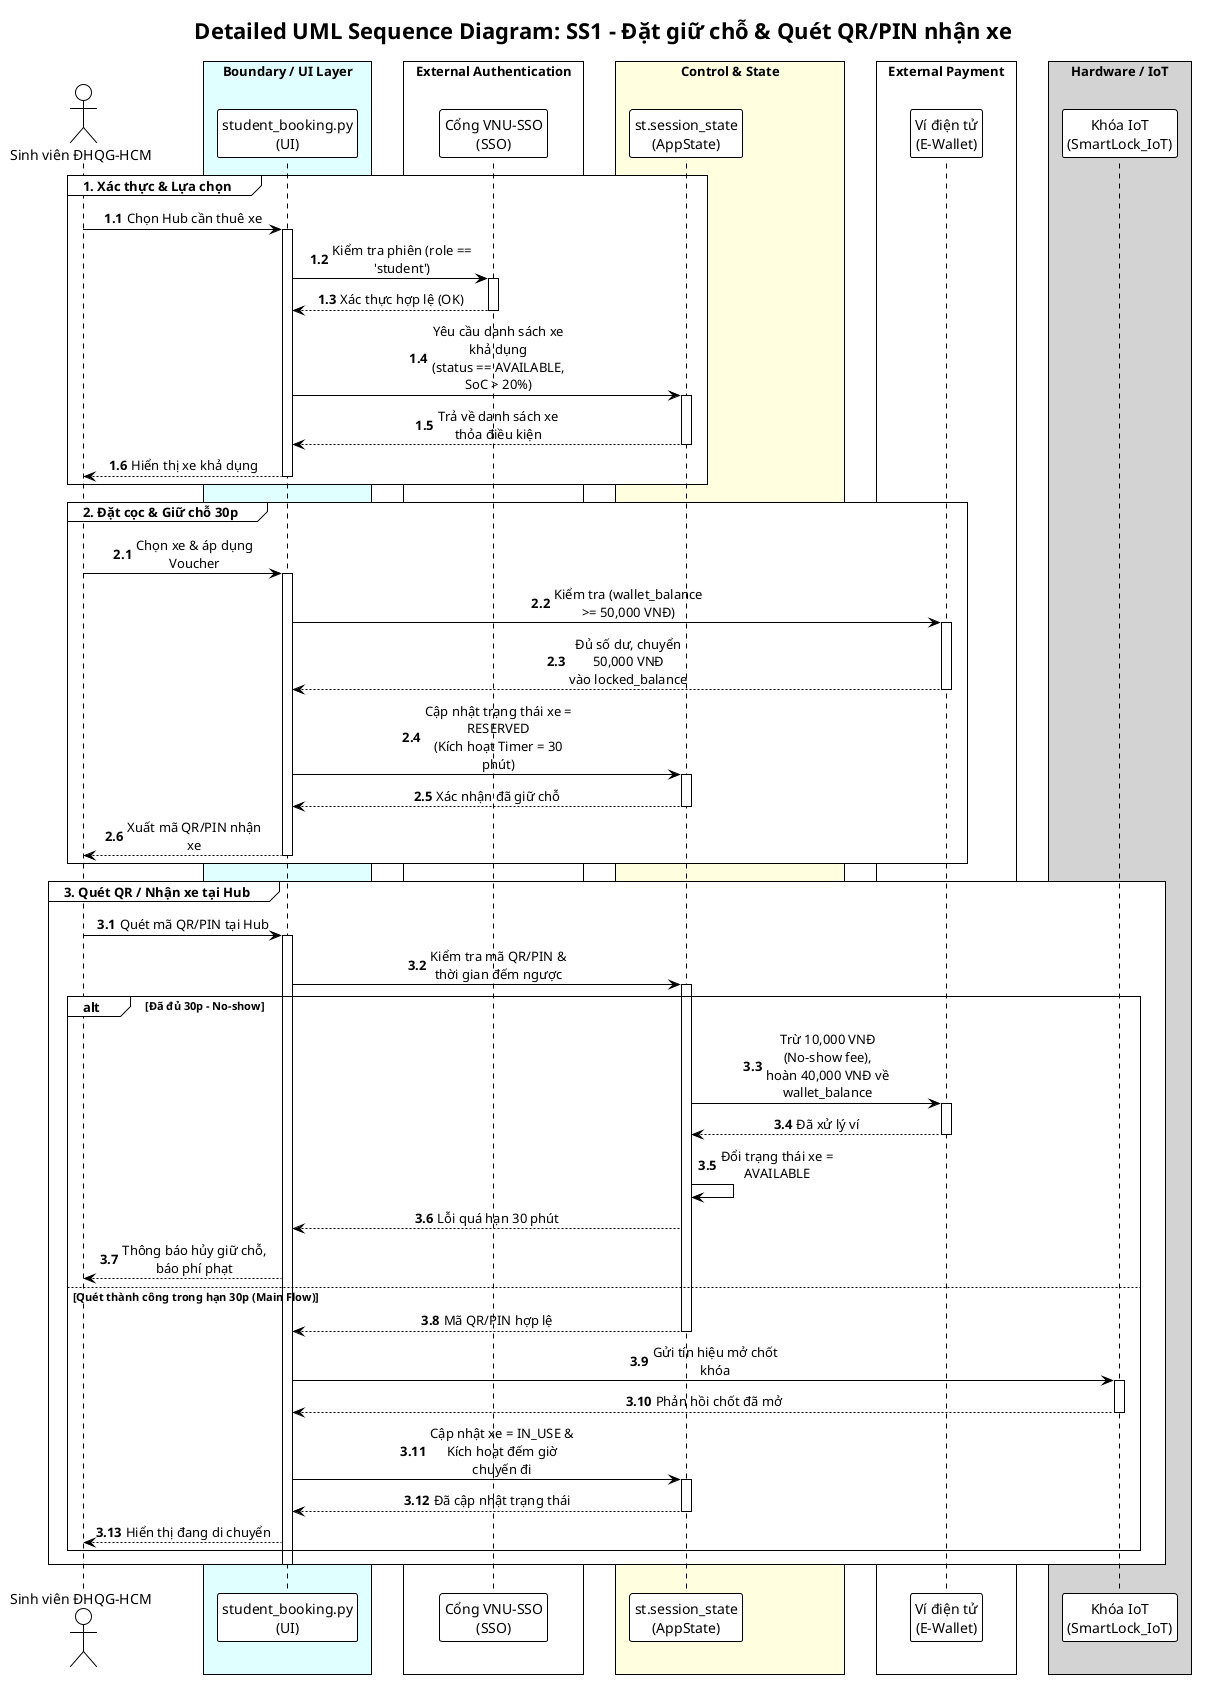
\includegraphics[width=0.88\textwidth]{Use-case detail-scenario/SS1/Sequence diagrams/UC_SS1_01_NguyenThanhDat_sequence.png}
    \caption{Sơ đồ Tuần tự Chi tiết -- UC\_SS1\_01 (Đặt xe \& Quét nhận xe)}
    \label{fig:seq-ss1-01}
\end{figure}

\begin{table}[H]
    \centering
    \small
    \renewcommand{\arraystretch}{1.25}
    \caption{Đặc tả Các Thông điệp Tương tác (Message Exchange Table) -- UC\_SS1\_01}
    \label{tab:msg-ss1-01}
    \begin{tabularx}{\textwidth}{|c|l|l|X|}
        \hline
        \textbf{Bước} & \textbf{Đối tượng Gửi} & \textbf{Đối tượng Nhận} & \textbf{Tên thông điệp / Dữ liệu trao đổi} \\
        \hline
        1 & Sinh viên & UI (student\_booking.py) & Chọn Hub, chọn xe điện và nhấn [Xác nhận Đặt xe] \\
        2 & UI & BookingController & \texttt{createReservation(studentId, hubId, vehicleType)} \\
        3 & BookingController & WalletService & \texttt{checkBalanceAndLockDeposit(studentId, 50000)} \\
        4 & WalletService & st.session\_state & Cập nhật số dư ví, trừ tiền cọc tạm giữ \\
        5 & BookingController & VehicleService & \texttt{lockVehicle(vehicleId, status="RESERVED", expire=15m)} \\
        6 & BookingController & UI & Trả về mã đặt chỗ + QR code nhận xe (hiệu lực 15 phút) \\
        7 & Sinh viên & SmartHub Gate IoT & Quét mã QR code hoặc nhập mã PIN tại trụ xe \\
        8 & SmartHub IoT & BookingController & \texttt{verifyUnlockRequest(pinCode, hubId)} \\
        9 & BookingController & SmartLock IoT & Lệnh mở khóa chốt cơ điện (\texttt{unlock()}), bật còi xác nhận \\
        10 & BookingController & st.session\_state & Chuyển trạng thái xe sang \texttt{IN\_USE}, bắt đầu tính giờ thuê \\
        \hline
    \end{tabularx}
\end{table}

\subsubsection{UC\_SS1\_02: Trả xe 1-chiều \& Quyết toán ví điện tử}
\paragraph{Mô tả nghiệp vụ:} Sinh viên đưa xe vào chốt khóa tại Hub bất kỳ. Cảm biến IoT xác thực vị trí chốt, đọc dung lượng pin hiện tại, tính cước thuê xe thực tế, hoàn lại phần cọc dư vào ví và xuất hóa đơn điện tử e-Invoice.
\begin{figure}[H]
    \centering
    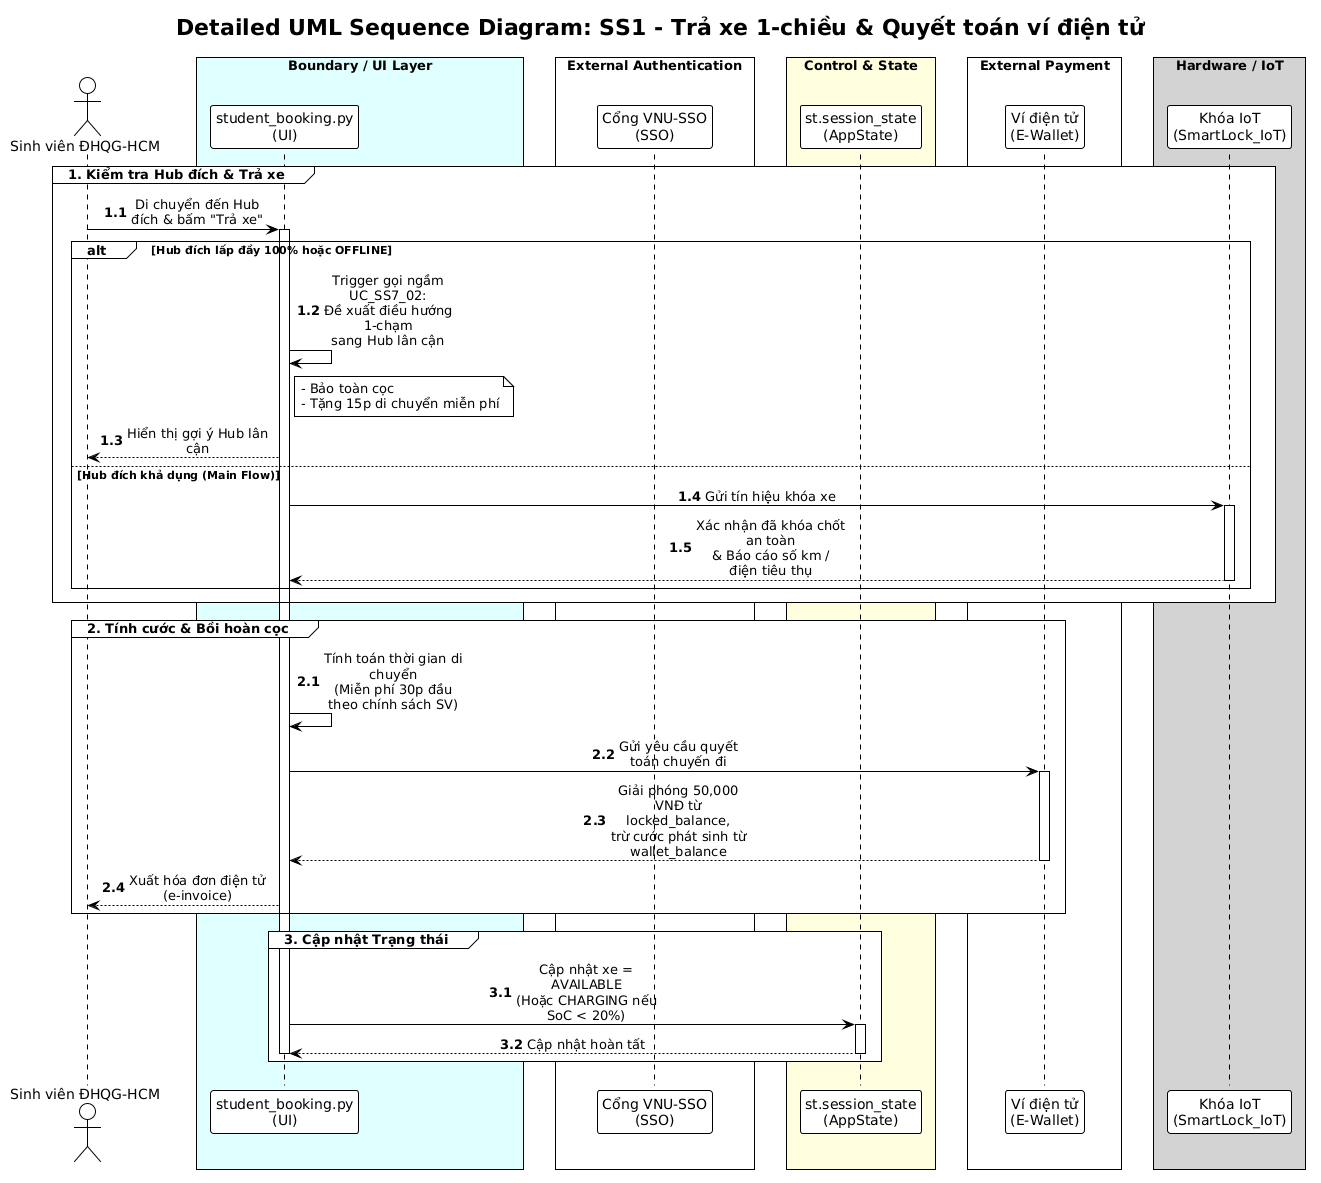
\includegraphics[width=0.88\textwidth]{Use-case detail-scenario/SS1/Sequence diagrams/UC_SS1_02_NguyenThanhDat_sequence.png}
    \caption{Sơ đồ Tuần tự Chi tiết -- UC\_SS1\_02 (Trả xe 1-chiều \& Quyết toán ví)}
    \label{fig:seq-ss1-02}
\end{figure}

\subsubsection{UC\_SS1\_03: Hủy đặt xe \& Hoàn 100\% cọc}
\paragraph{Mô tả nghiệp vụ:} Sinh viên chủ động hủy đặt chỗ trong thời hạn 15 phút hoặc khi hết hạn 15 phút mà sinh viên không đến nhận xe, hệ thống tự động giải phóng xe về trạng thái \texttt{AVAILABLE} và hoàn 100\% tiền cọc 50.000 VNĐ.
\begin{figure}[H]
    \centering
    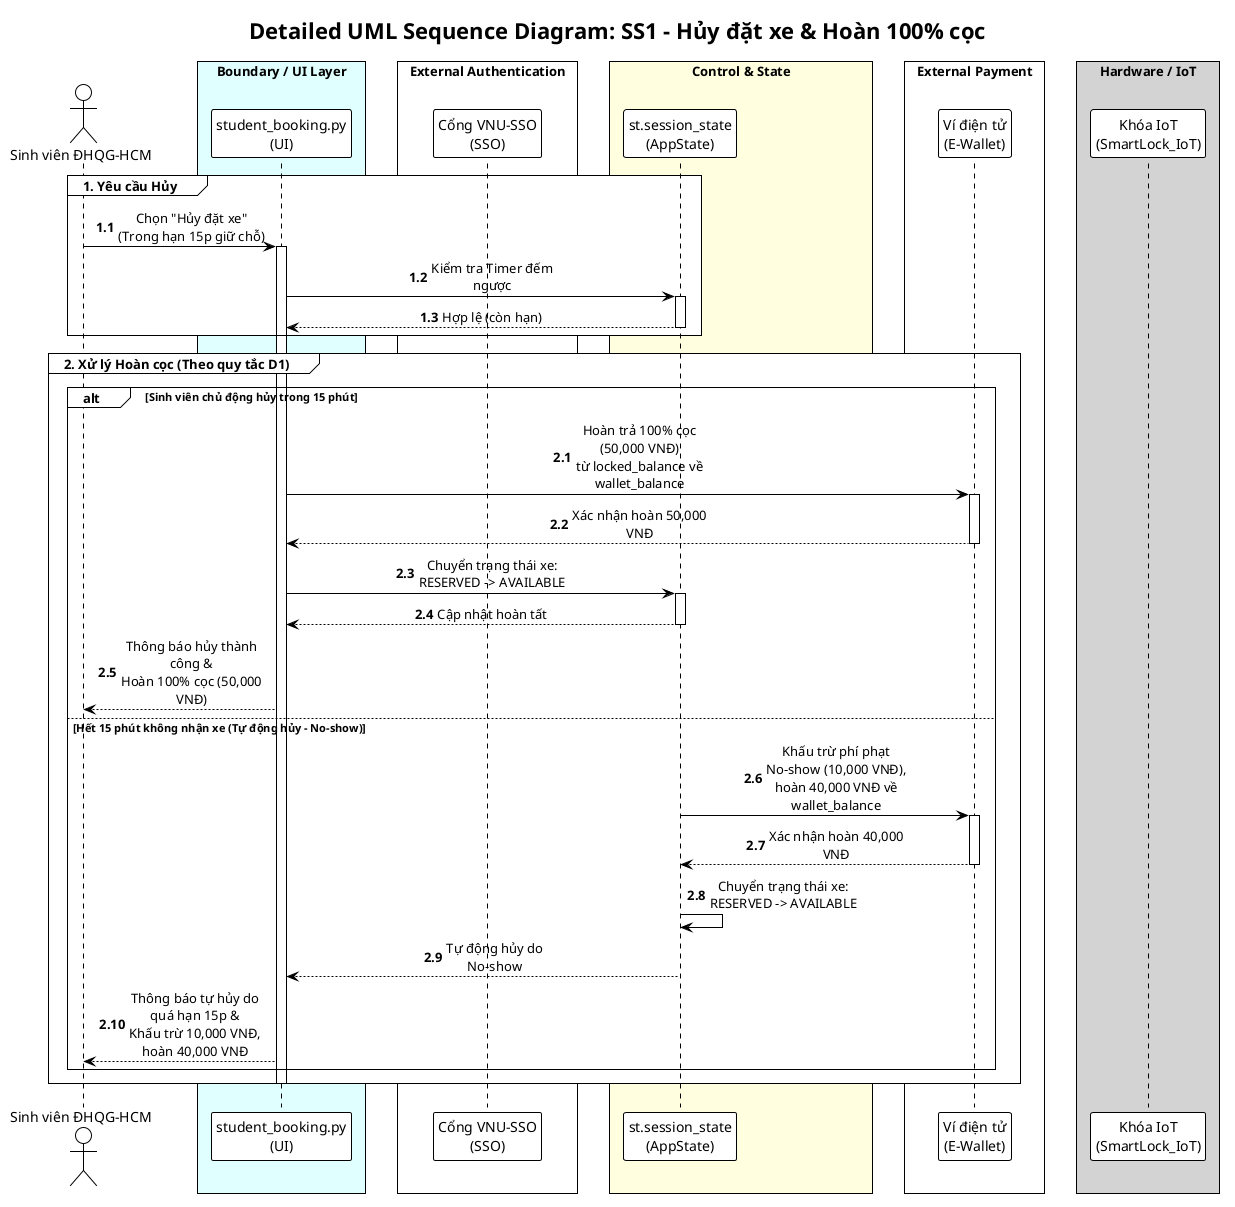
\includegraphics[width=0.88\textwidth]{Use-case detail-scenario/SS1/Sequence diagrams/UC_SS1_03_NguyenThanhDat_sequence.png}
    \caption{Sơ đồ Tuần tự Chi tiết -- UC\_SS1\_03 (Hủy đặt xe \& Hoàn cọc 100\%)}
    \label{fig:seq-ss1-03}
\end{figure}

% ------------------------------------------------------------
% 2.2 SS2 - Nguyễn Anh Tài
% ------------------------------------------------------------
\subsection{Phân hệ SS2: Đăng ký Sạc \& Đỗ xe cá nhân (Nguyễn Anh Tài)}

\subsubsection{UC\_SS2\_01: Đăng ký xe EV cá nhân}
\paragraph{Mô tả nghiệp vụ:} Sinh viên khai báo biển số xe, loại xe (VinFast, Dat Bike...), dung lượng pin và ảnh giấy đăng ký xe; hệ thống kiểm tra trùng lặp và lưu trữ hồ sơ phương tiện.
\begin{figure}[H]
    \centering
    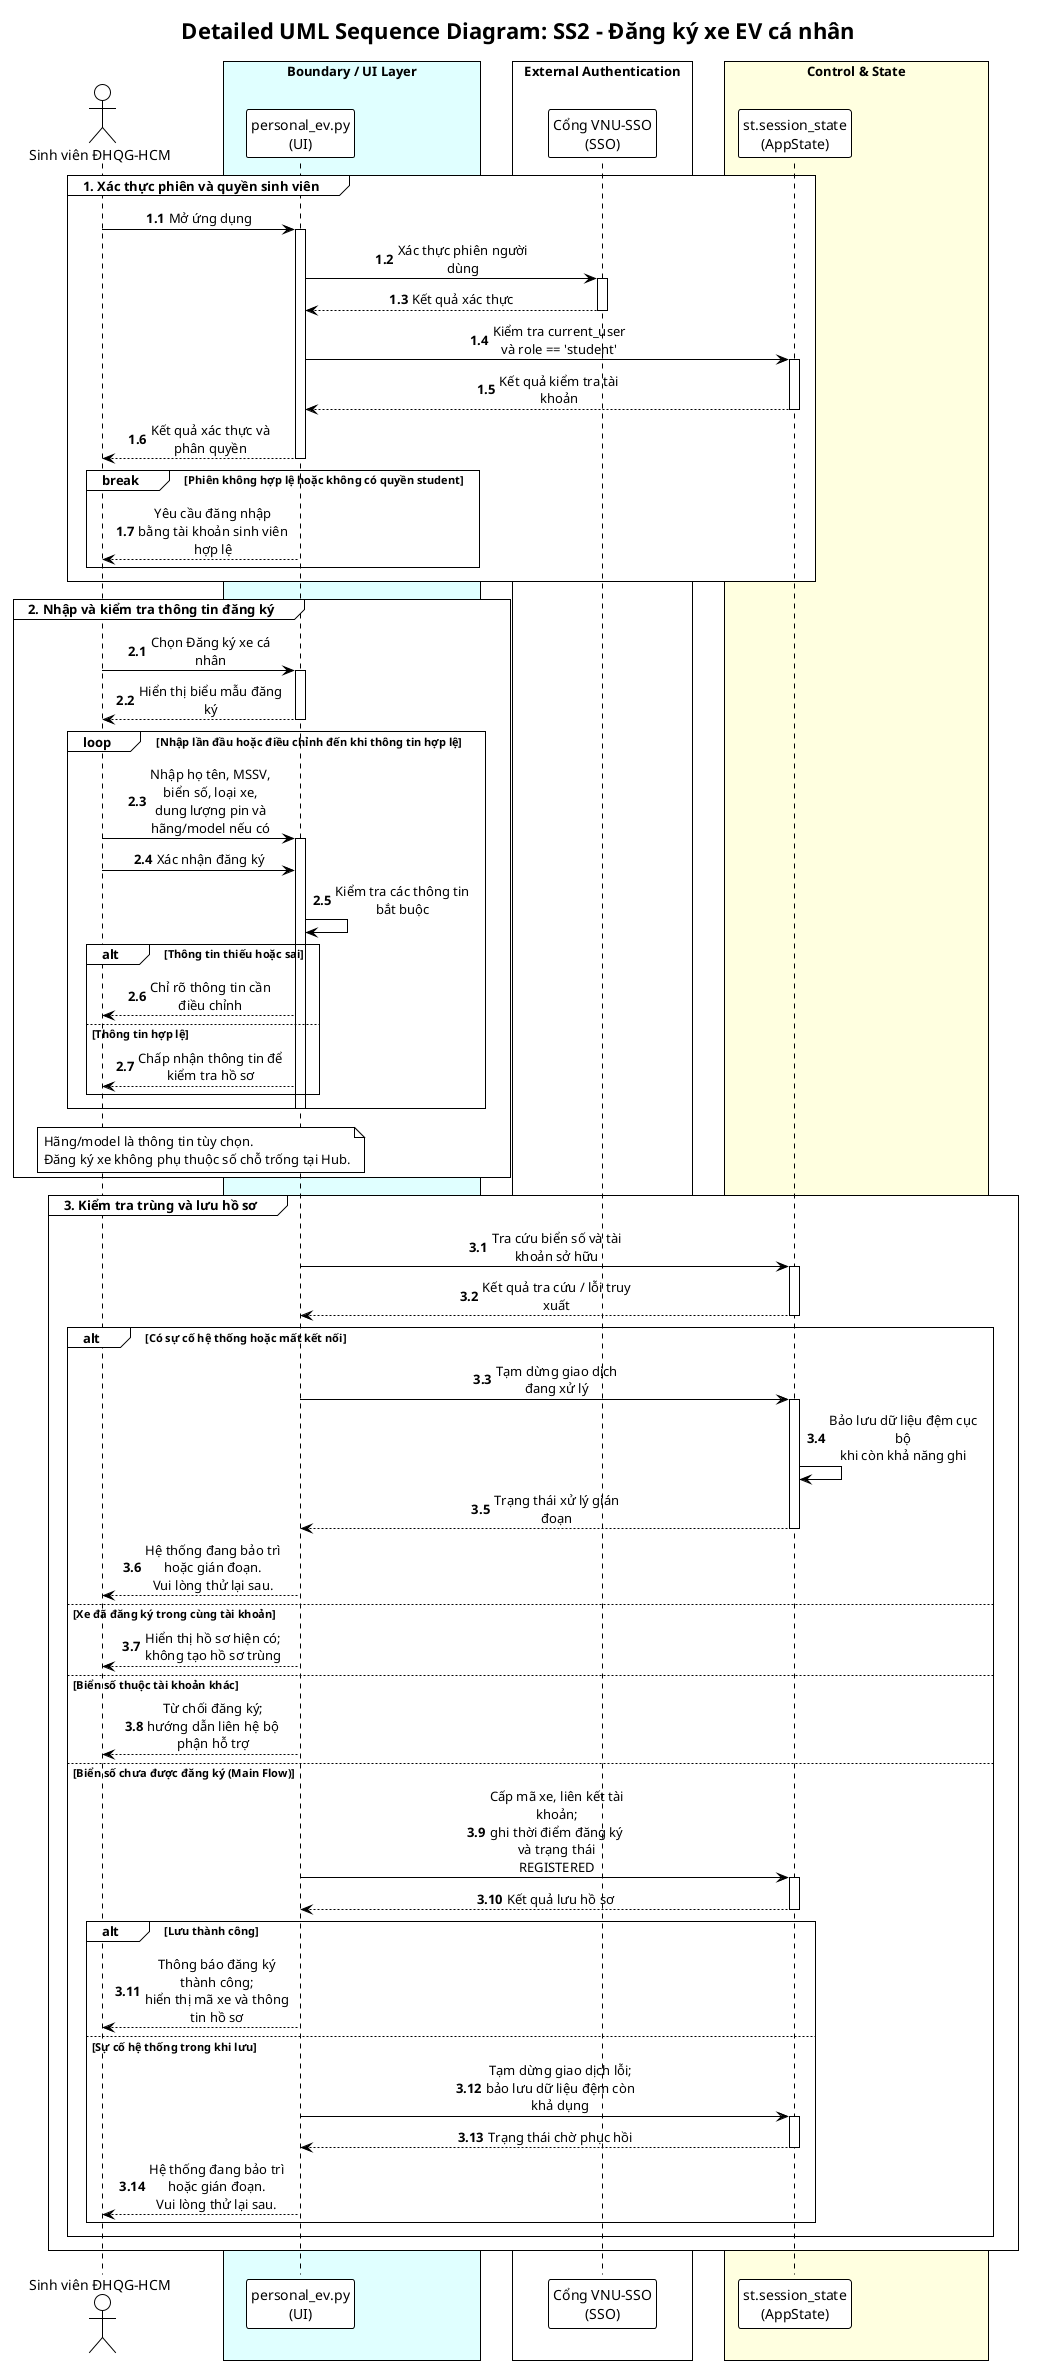
\includegraphics[width=0.88\textwidth]{Use-case detail-scenario/SS2/Sequence diagrams/UC_SS2_01_NguyenAnhTai_sequence.png}
    \caption{Sơ đồ Tuần tự Chi tiết -- UC\_SS2\_01 (Đăng ký xe EV cá nhân)}
    \label{fig:seq-ss2-01}
\end{figure}

\subsubsection{UC\_SS2\_02: Đặt chỗ đỗ và nhu cầu sạc xe EV cá nhân}
\paragraph{Mô tả nghiệp vụ:} Sinh viên chọn Hub đích, thời gian gửi xe và lựa chọn dịch vụ sạc có/không có sạc; hệ thống khóa giữ chỗ đỗ và slot trụ sạc tương ứng.
\begin{figure}[H]
    \centering
    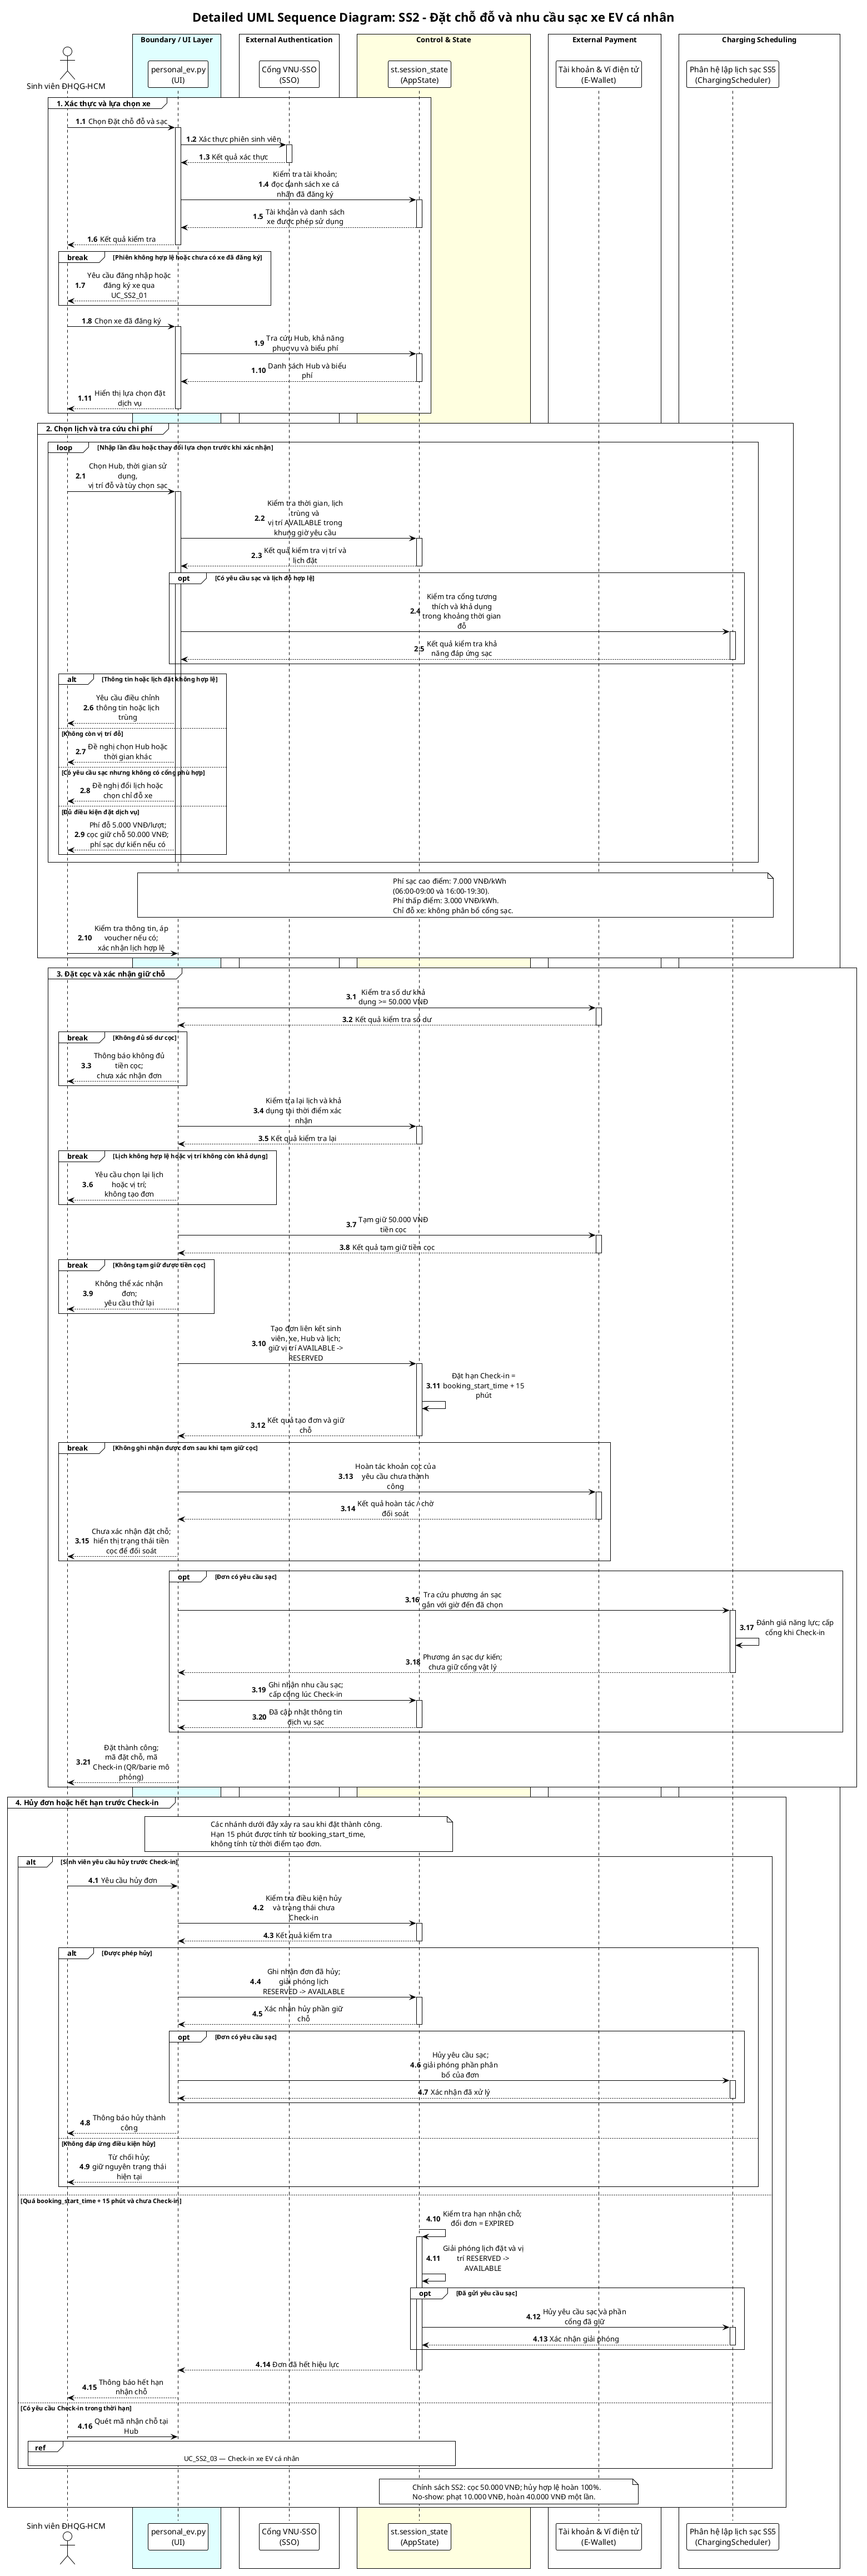
\includegraphics[width=0.88\textwidth]{Use-case detail-scenario/SS2/Sequence diagrams/UC_SS2_02_NguyenAnhTai_sequence.png}
    \caption{Sơ đồ Tuần tự Chi tiết -- UC\_SS2\_02 (Đặt chỗ đỗ \& Lịch sạc xe cá nhân)}
    \label{fig:seq-ss2-02}
\end{figure}

\subsubsection{UC\_SS2\_03: Check-in xe EV cá nhân tại Hub}
\paragraph{Mô tả nghiệp vụ:} Camera ANPR tại cổng Hub nhận diện biển số xe trùng khớp với phiên đặt trước, mở barie tự động và chỉ dẫn sinh viên vào đúng vị trí slot đỗ/sạc.
\begin{figure}[H]
    \centering
    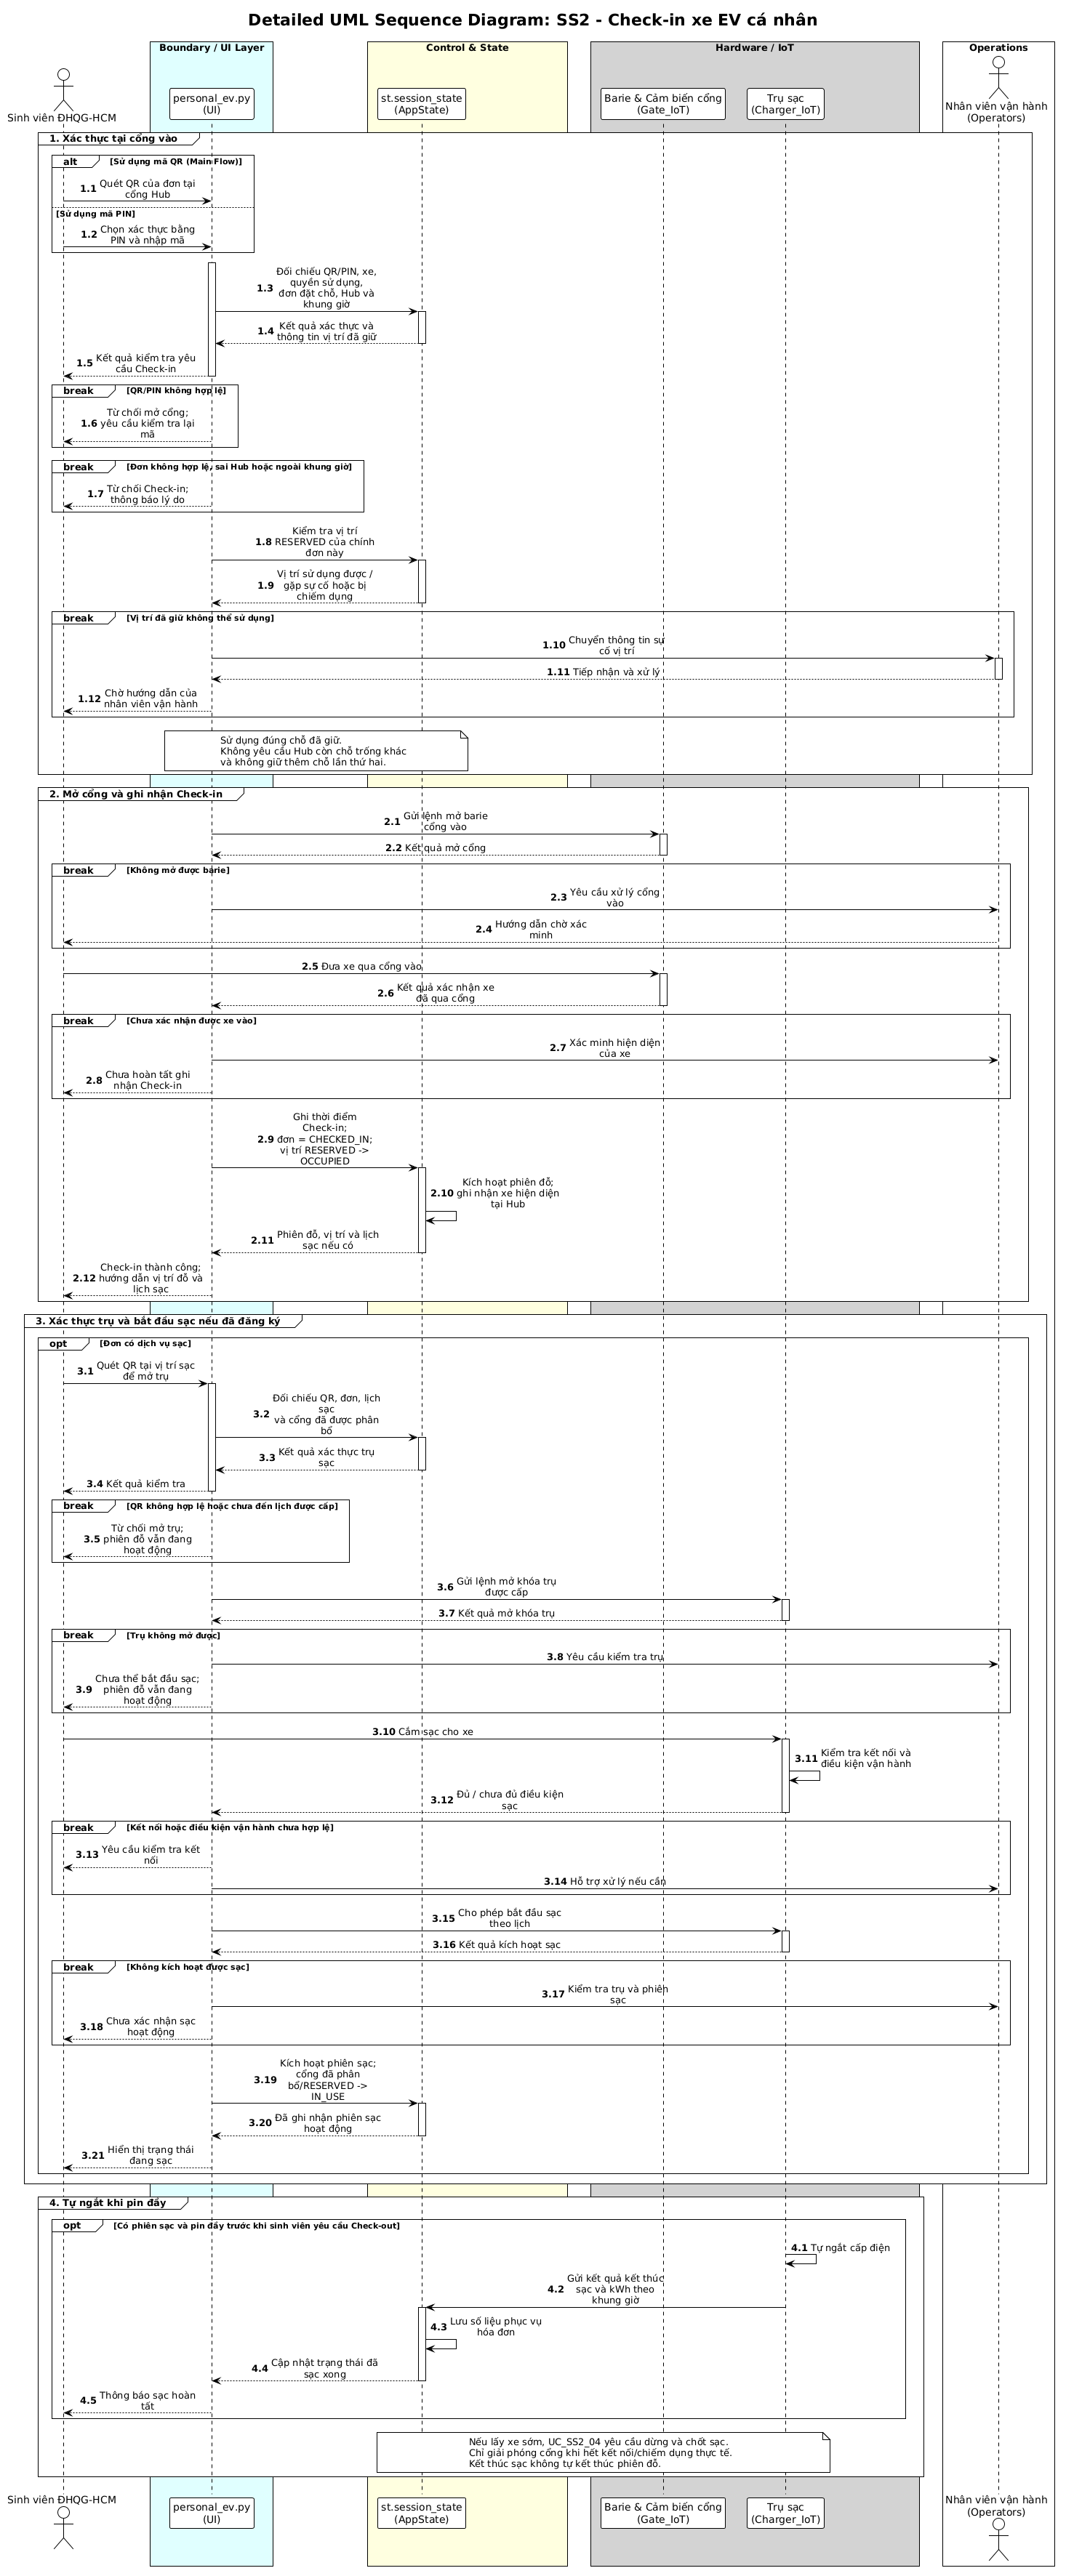
\includegraphics[width=0.88\textwidth]{Use-case detail-scenario/SS2/Sequence diagrams/UC_SS2_03_NguyenAnhTai_sequence.png}
    \caption{Sơ đồ Tuần tự Chi tiết -- UC\_SS2\_03 (Check-in xe EV cá nhân tại Hub)}
    \label{fig:seq-ss2-03}
\end{figure}

\subsubsection{UC\_SS2\_04: Check-out và thanh toán dịch vụ xe cá nhân}
\paragraph{Mô tả nghiệp vụ:} Khi sinh viên lấy xe ra, hệ thống tính toán tổng thời gian đỗ, điện năng tiêu thụ (kWh), tự động trừ ví điện tử và mở barie ra.
\begin{figure}[H]
    \centering
    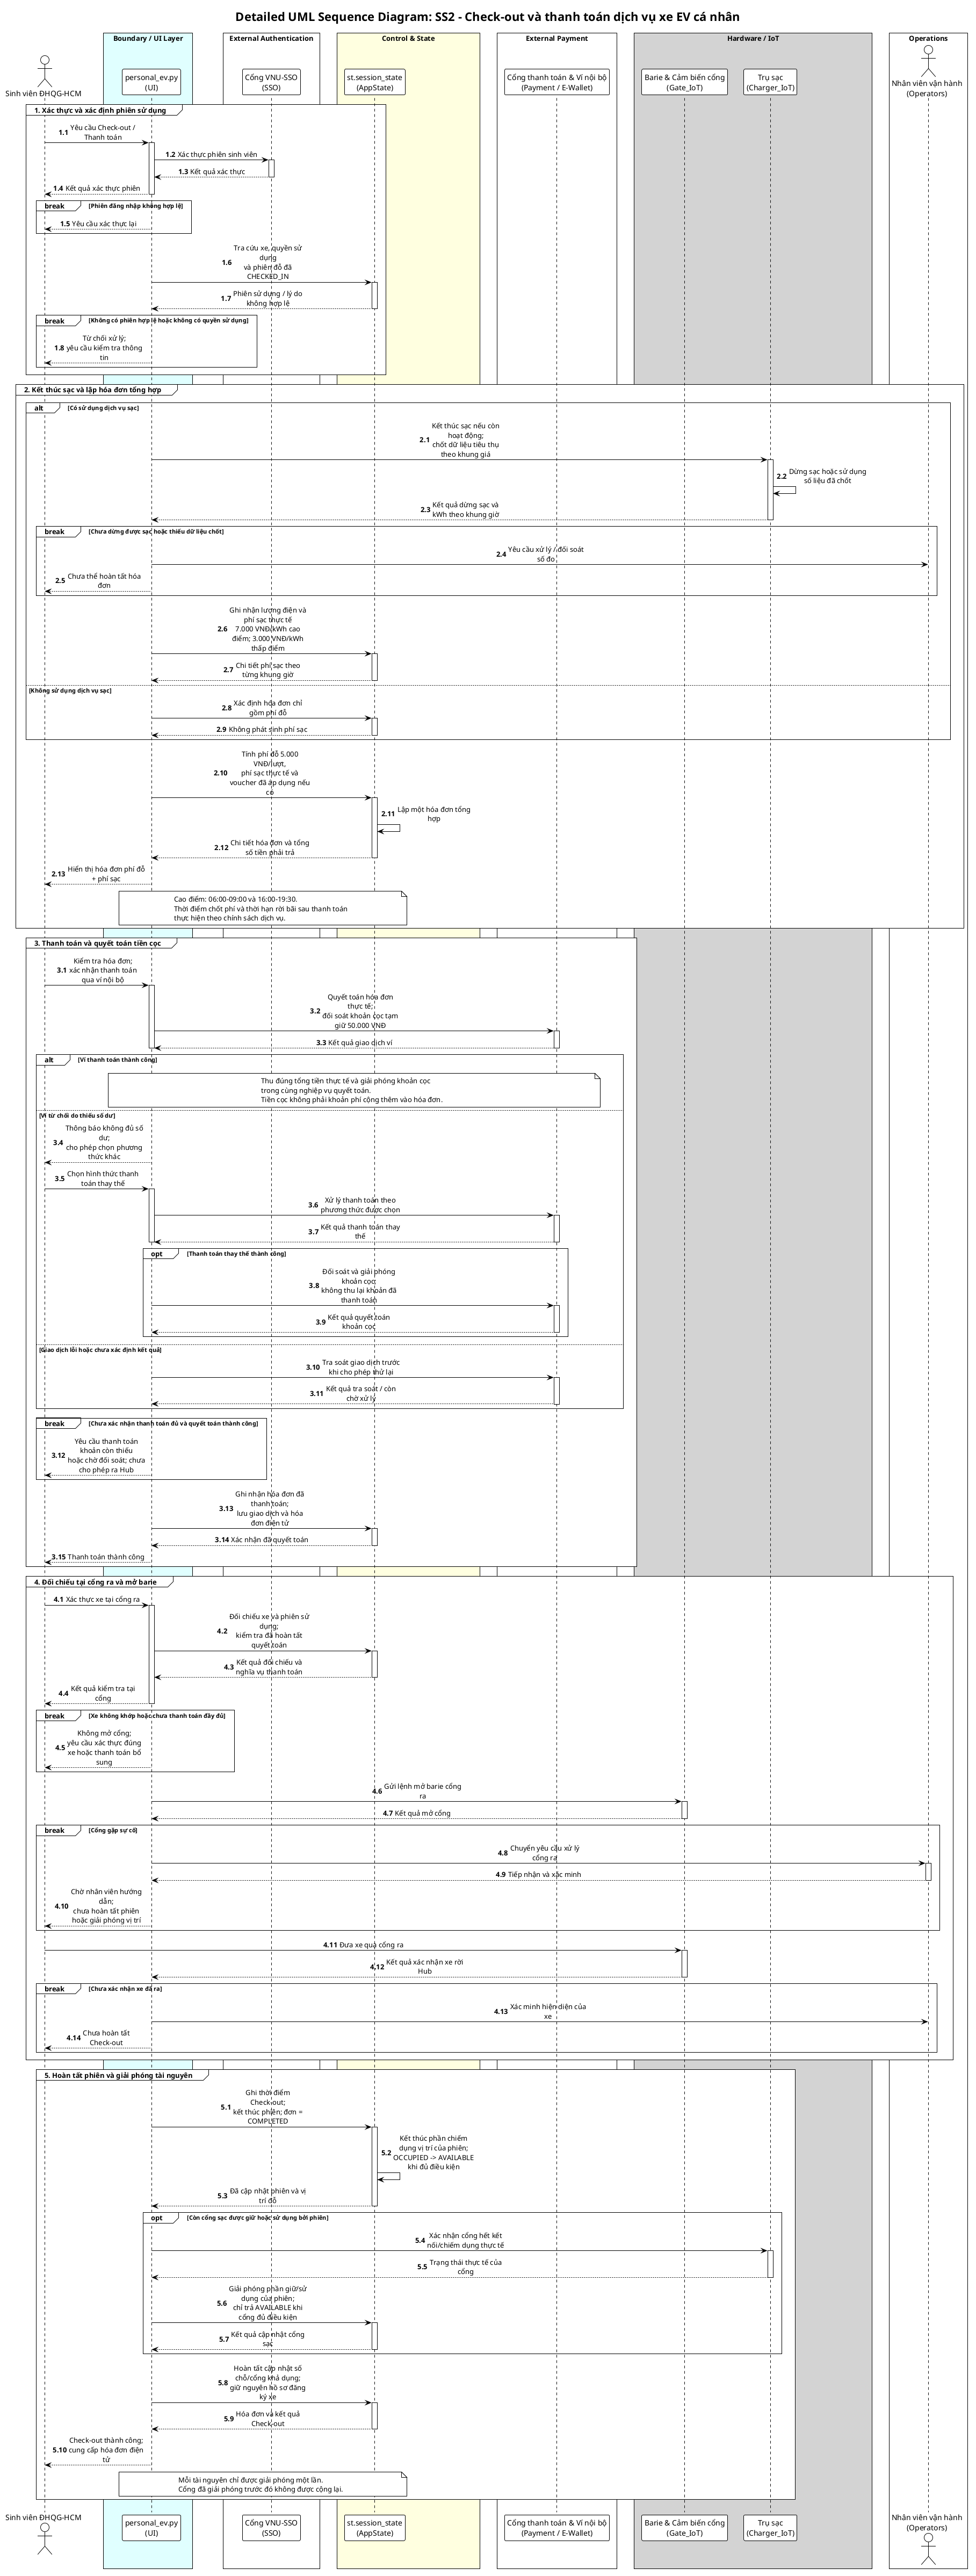
\includegraphics[width=0.88\textwidth]{Use-case detail-scenario/SS2/Sequence diagrams/UC_SS2_04_NguyenAnhTai_sequence.png}
    \caption{Sơ đồ Tuần tự Chi tiết -- UC\_SS2\_04 (Check-out \& Thanh toán dịch vụ xe)}
    \label{fig:seq-ss2-04}
\end{figure}

% ------------------------------------------------------------
% 2.3 SS3 - Phạm Tiến Đạt
% ------------------------------------------------------------
\subsection{Phân hệ SS3: Giám sát Mạng lưới Hub (Phạm Tiến Đạt)}

\subsubsection{UC\_SS3\_01: Giám sát trạng thái Hub theo thời gian thực}
\paragraph{Mô tả nghiệp vụ:} Dashboard liên tục truy vấn dữ liệu từ cảm biến IoT và trạng thái xe trong \texttt{st.session\_state["hubs"]}, tính toán tỷ lệ lấp đầy, số xe hoạt động và doanh thu tạm tính.
\begin{figure}[H]
    \centering
    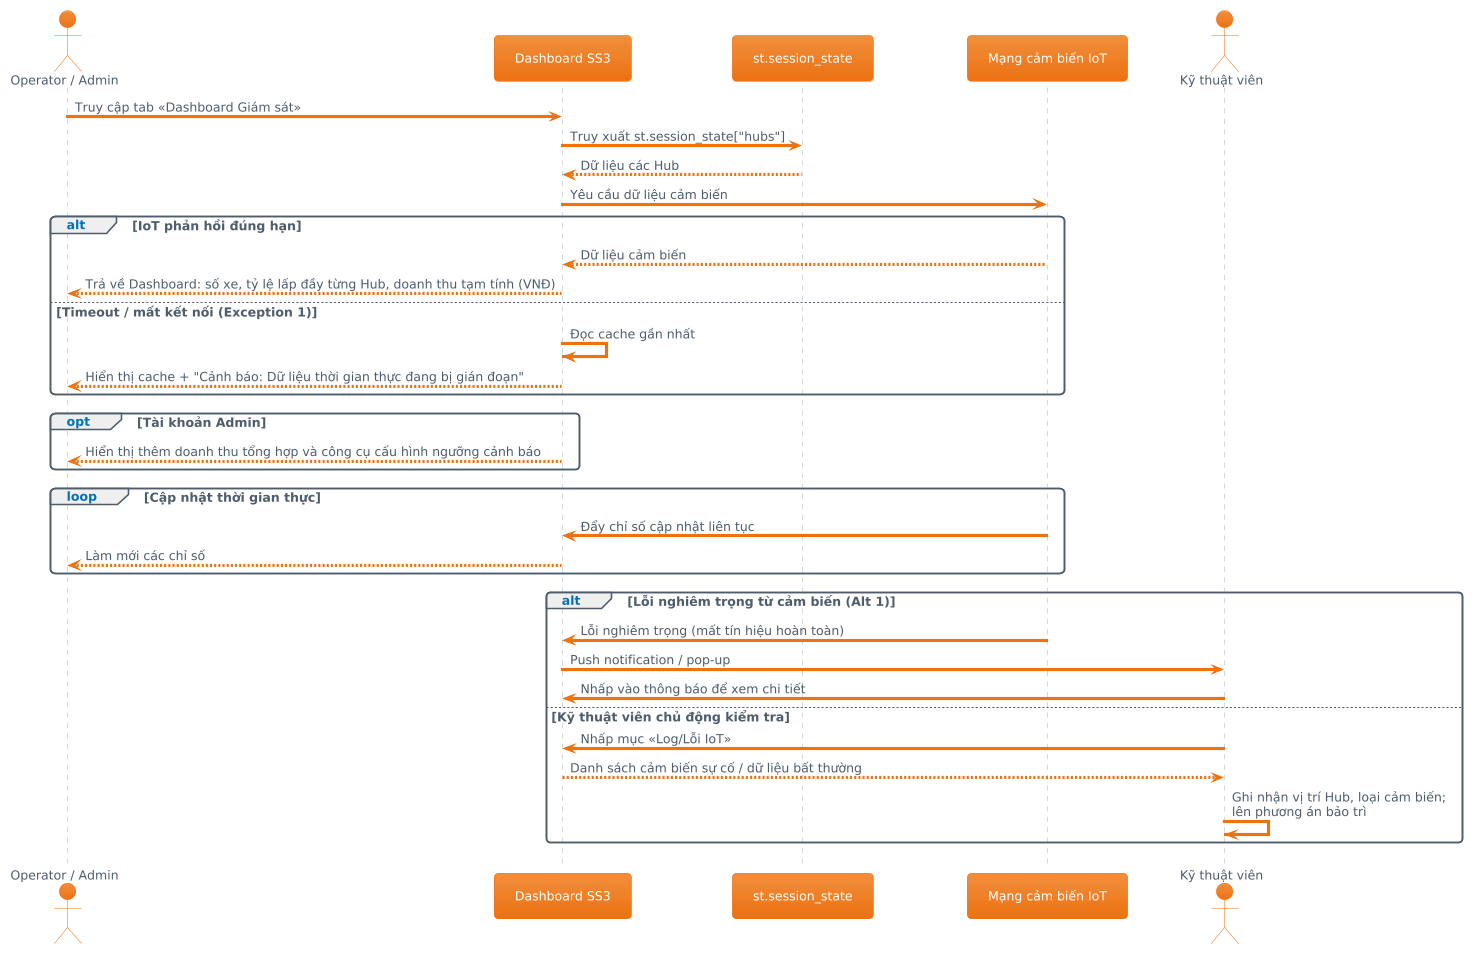
\includegraphics[width=0.88\textwidth]{Use-case detail-scenario/SS3/Sequence diagrams/UC_SS3_01_PhamTienDat_sequence.png}
    \caption{Sơ đồ Tuần tự Chi tiết -- UC\_SS3\_01 (Giám sát trạng thái Hub thời gian thực)}
    \label{fig:seq-ss3-01}
\end{figure}

\subsubsection{UC\_SS3\_02: Cảnh báo quá tải \& Đề xuất điều phối}
\paragraph{Mô tả nghiệp vụ:} Khi tỷ lệ lấp đầy tại một Hub vượt ngưỡng $\ge 85\%$, hệ thống tự động đẩy cảnh báo màu đỏ lên Dashboard và khởi tạo đề xuất lệnh điều xe sang phân hệ SS4.
\begin{figure}[H]
    \centering
    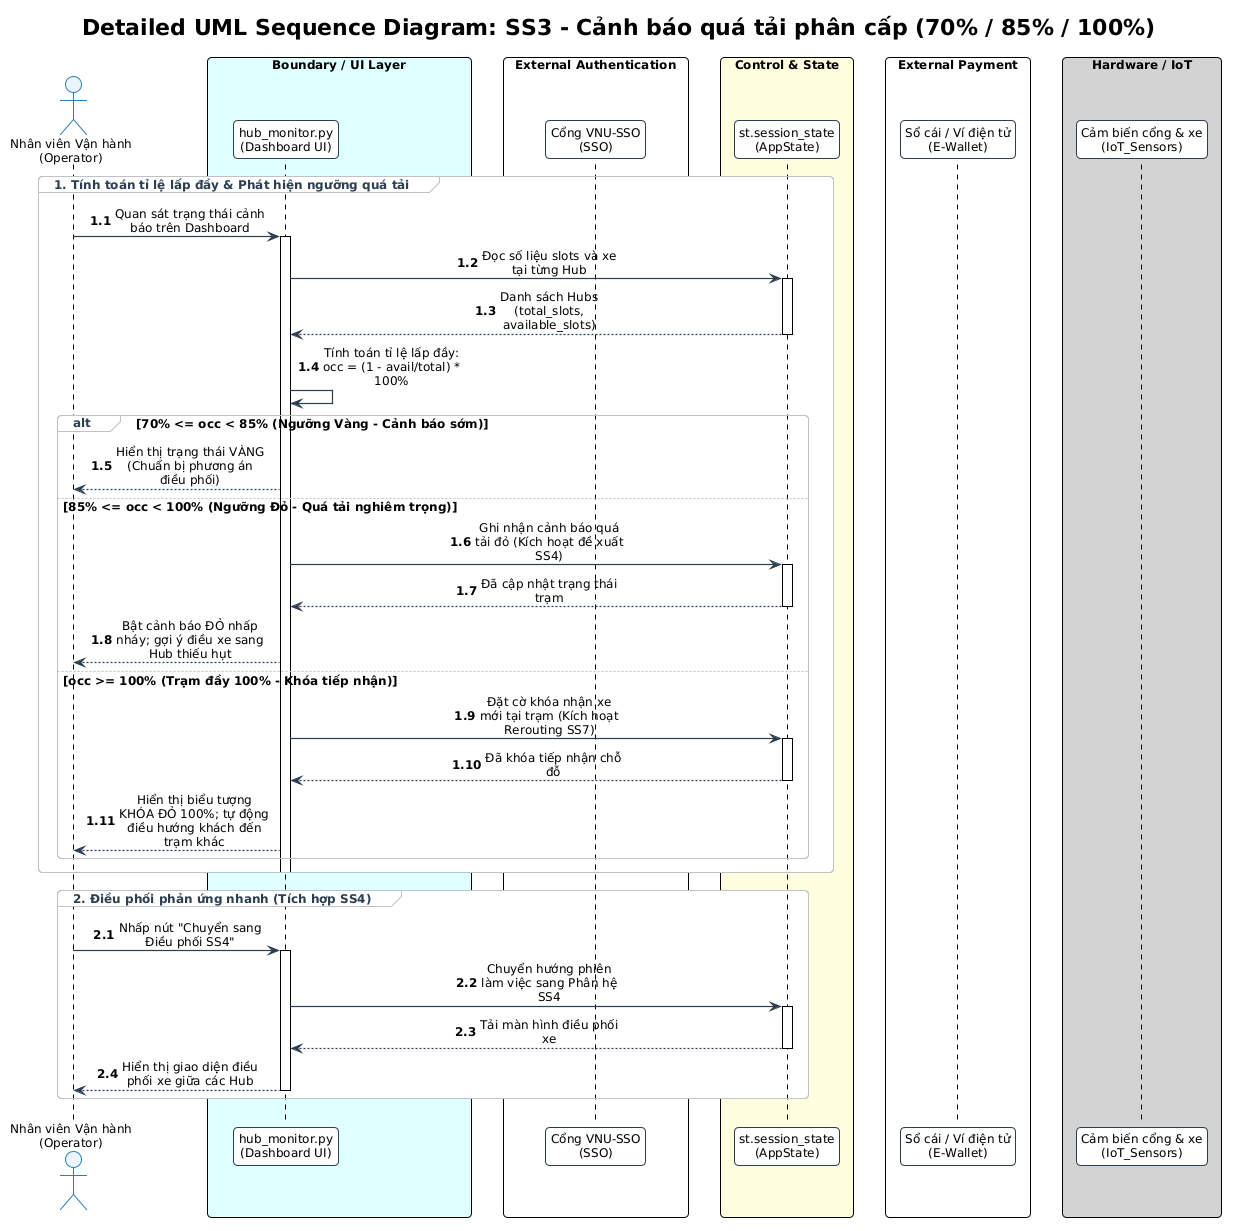
\includegraphics[width=0.88\textwidth]{Use-case detail-scenario/SS3/Sequence diagrams/UC_SS3_02_PhamTienDat_sequence.png}
    \caption{Sơ đồ Tuần tự Chi tiết -- UC\_SS3\_02 (Cảnh báo quá tải \& Đề xuất điều phối)}
    \label{fig:seq-ss3-02}
\end{figure}

% ------------------------------------------------------------
% 2.4 SS4 - Đặng Hoàng Quý Nhân
% ------------------------------------------------------------
\subsection{Phân hệ SS4: Điều phối \& Xử lý Sự cố (Đặng Hoàng Quý Nhân)}

\subsubsection{UC\_SS4\_01: Lập lệnh điều phối phương tiện giữa các Hub}
\paragraph{Mô tả nghiệp vụ:} Điều hành viên tiếp nhận cảnh báo quá tải, chọn Hub nguồn thừa xe và Hub đích thiếu xe, lập lệnh điều phối và phân bổ xe tải chuyên dụng thực hiện luân chuyển.
\begin{figure}[H]
    \centering
    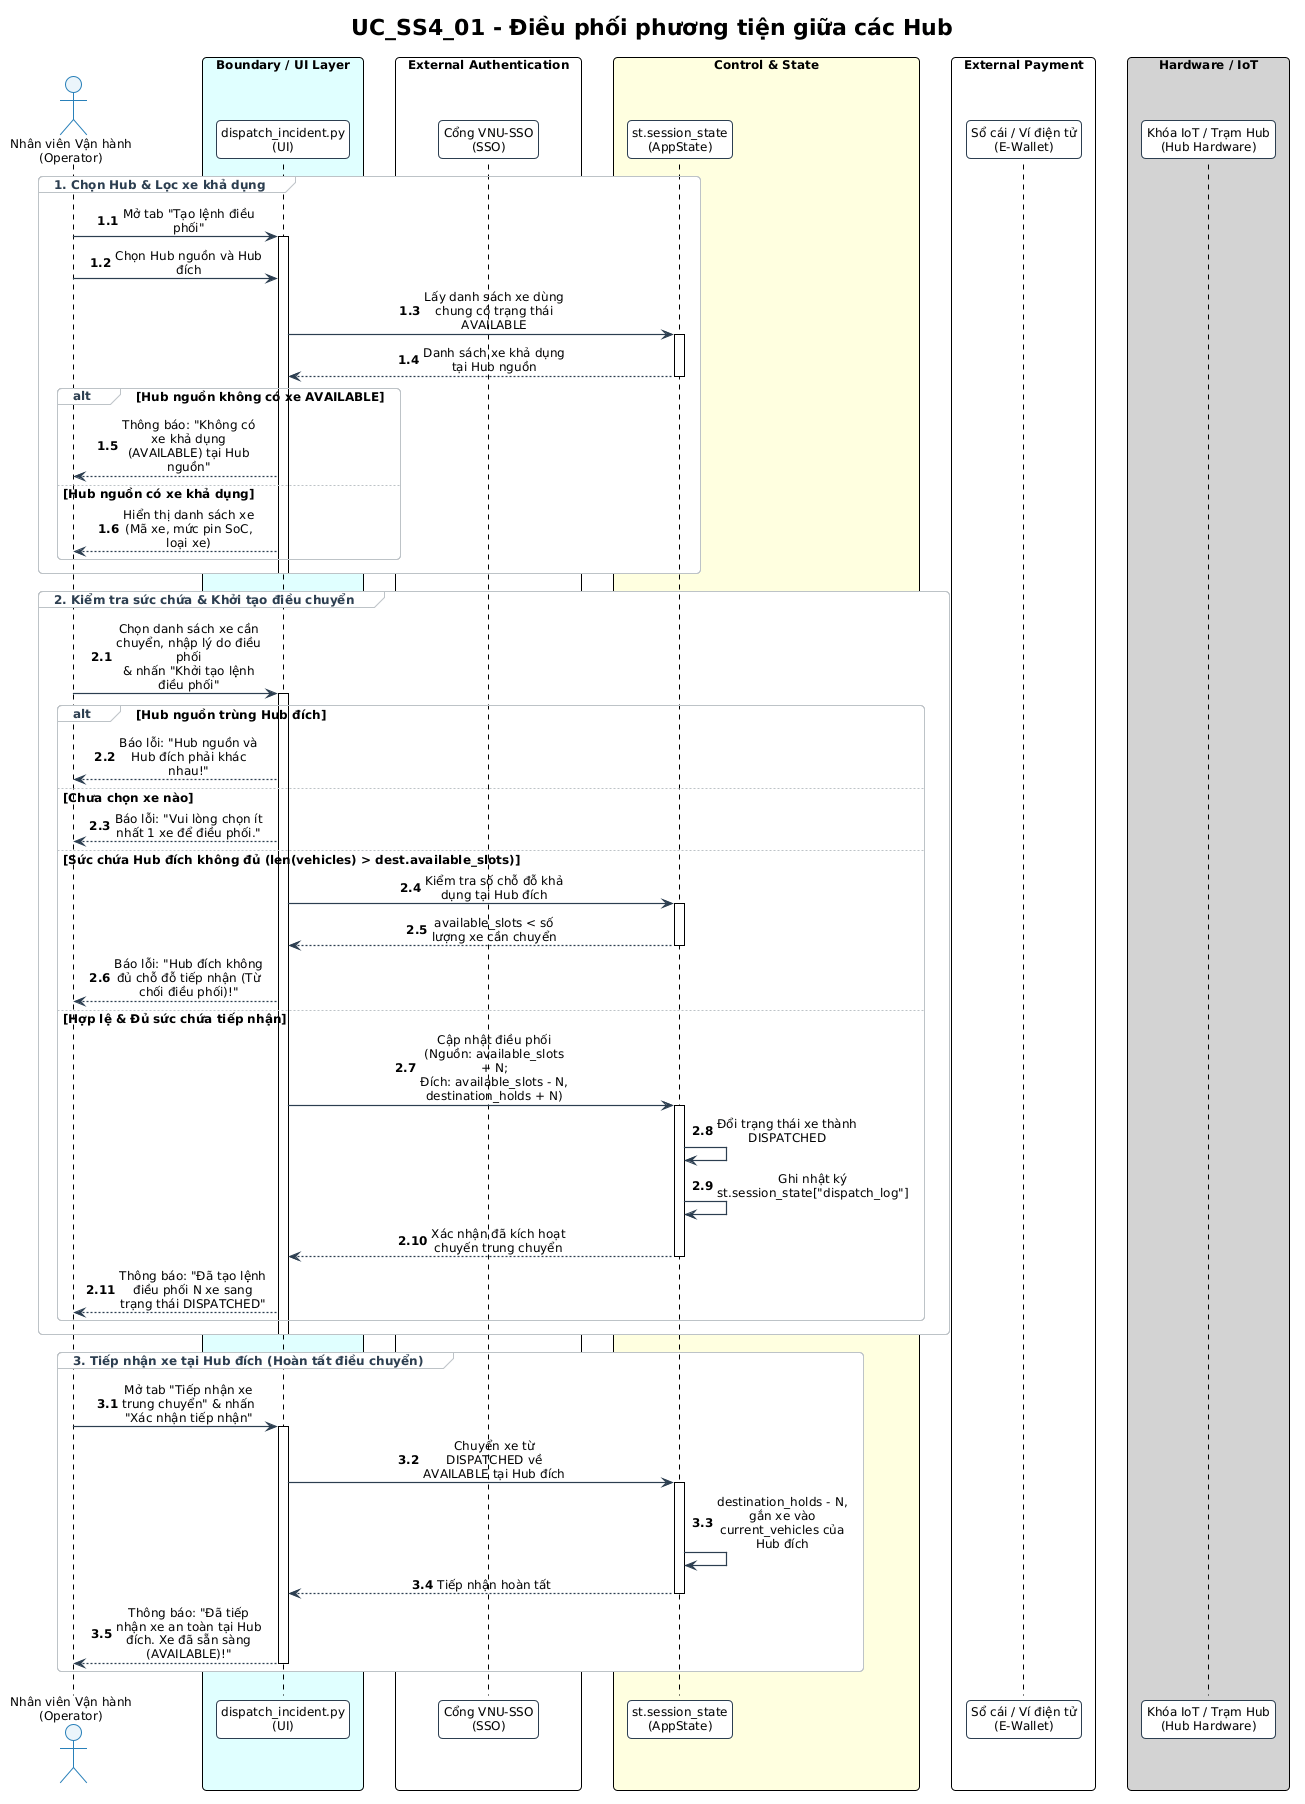
\includegraphics[width=0.88\textwidth]{Use-case detail-scenario/SS4/Sequence diagrams/UC_SS4_01_sequence.png}
    \caption{Sơ đồ Tuần tự Chi tiết -- UC\_SS4\_01 (Lập lệnh điều phối phương tiện)}
    \label{fig:seq-ss4-01}
\end{figure}

\subsubsection{UC\_SS4\_02: Báo cáo \& Xử lý sự cố kỹ thuật phương tiện}
\paragraph{Mô tả nghiệp vụ:} Khi có báo cáo hỏng xe từ sinh viên hoặc cảm biến pin quá nhiệt, hệ thống lập tức khóa xe khỏi danh sách cho thuê, phân công Kỹ thuật viên kiểm tra và sửa chữa.
\begin{figure}[H]
    \centering
    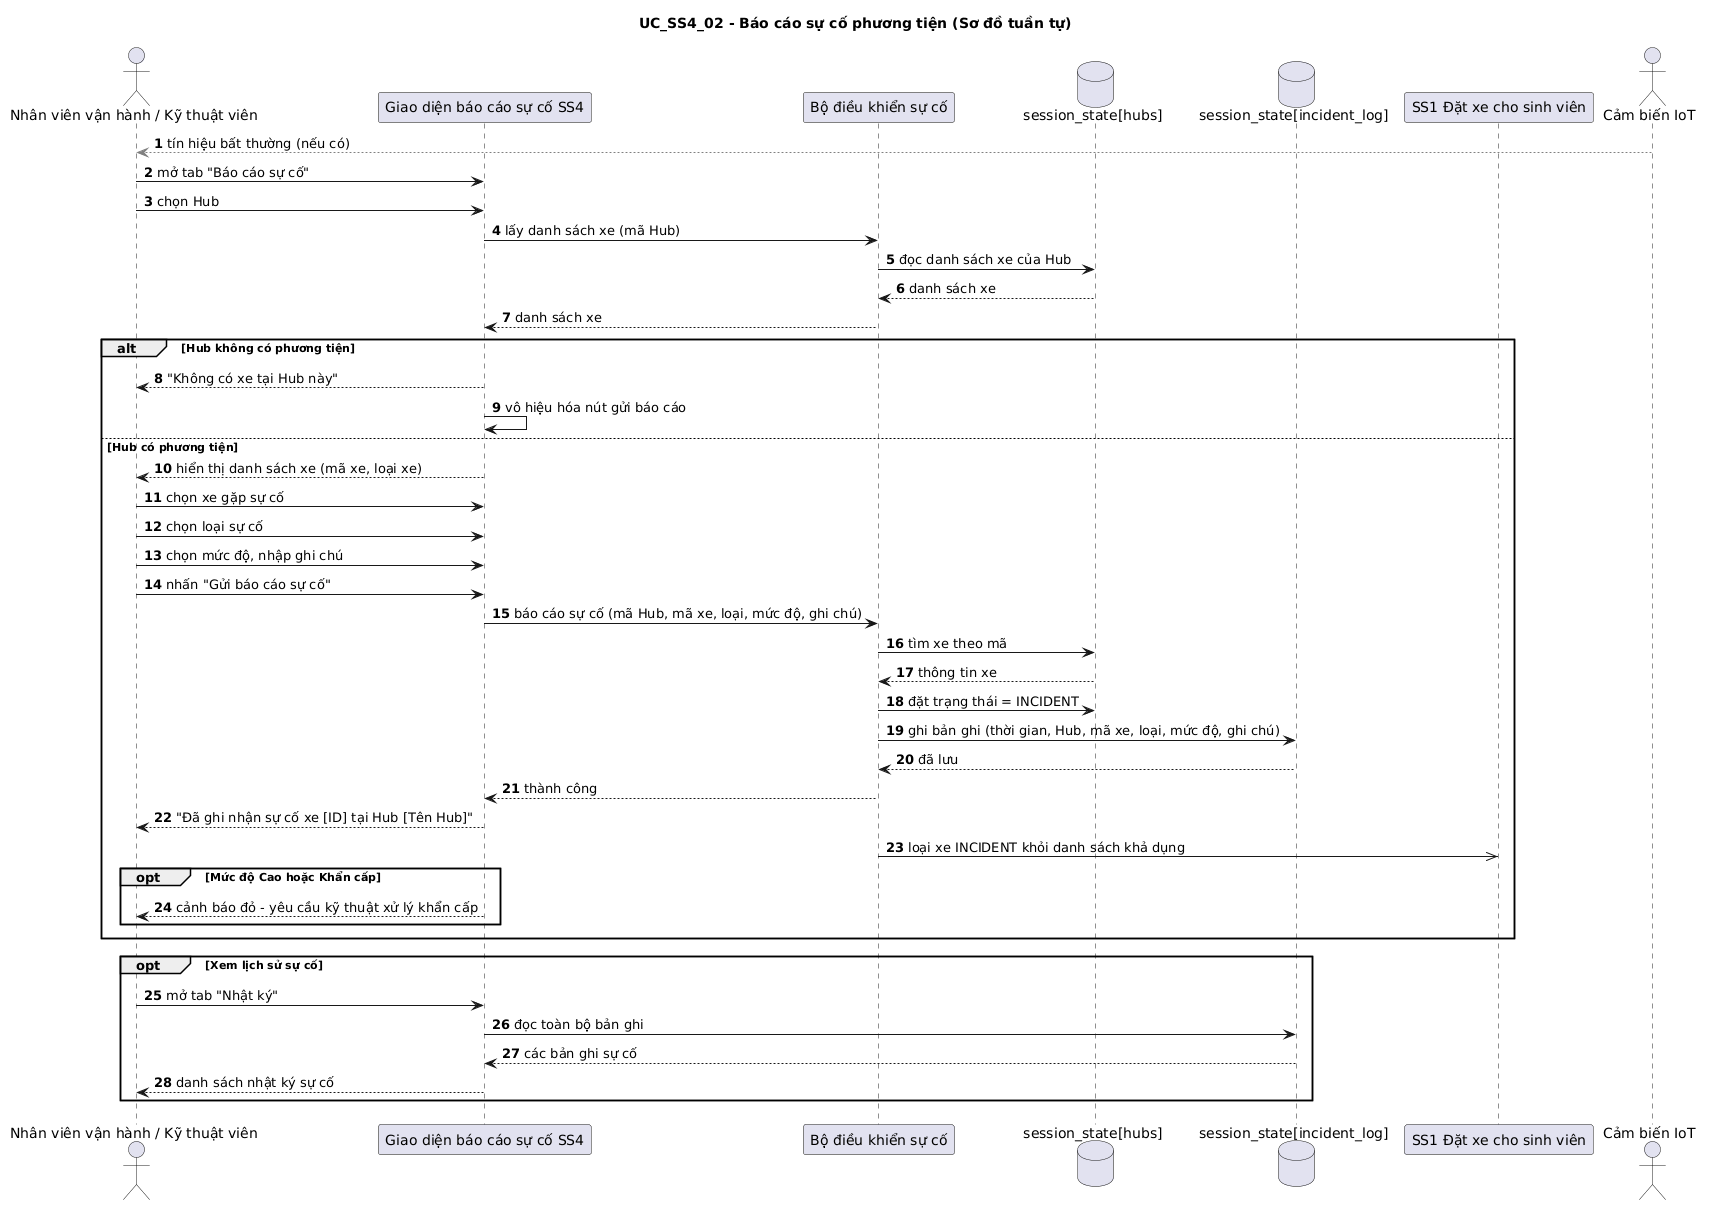
\includegraphics[width=0.88\textwidth]{Use-case detail-scenario/SS4/Sequence diagrams/UC_SS4_02_sequence.png}
    \caption{Sơ đồ Tuần tự Chi tiết -- UC\_SS4\_02 (Báo cáo \& Xử lý sự cố kỹ thuật xe)}
    \label{fig:seq-ss4-02}
\end{figure}

% ------------------------------------------------------------
% 2.5 SS5 - Dương Đăng Khoa
% ------------------------------------------------------------
\subsection{Phân hệ SS5: Lập lịch Sạc Thông minh (Dương Đăng Khoa)}

\subsubsection{UC\_SS5\_01: Lập lịch ưu tiên sạc tự động}
\paragraph{Mô tả nghiệp vụ:} Thuật toán tối ưu hóa lịch sạc kiểm tra mức pin của từng xe trong hàng đợi, tự động ưu tiên cấp điện áp cao cho các xe có mức pin dưới 20\% và xếp lịch sạc ngoài giờ cao điểm.
\begin{figure}[H]
    \centering
    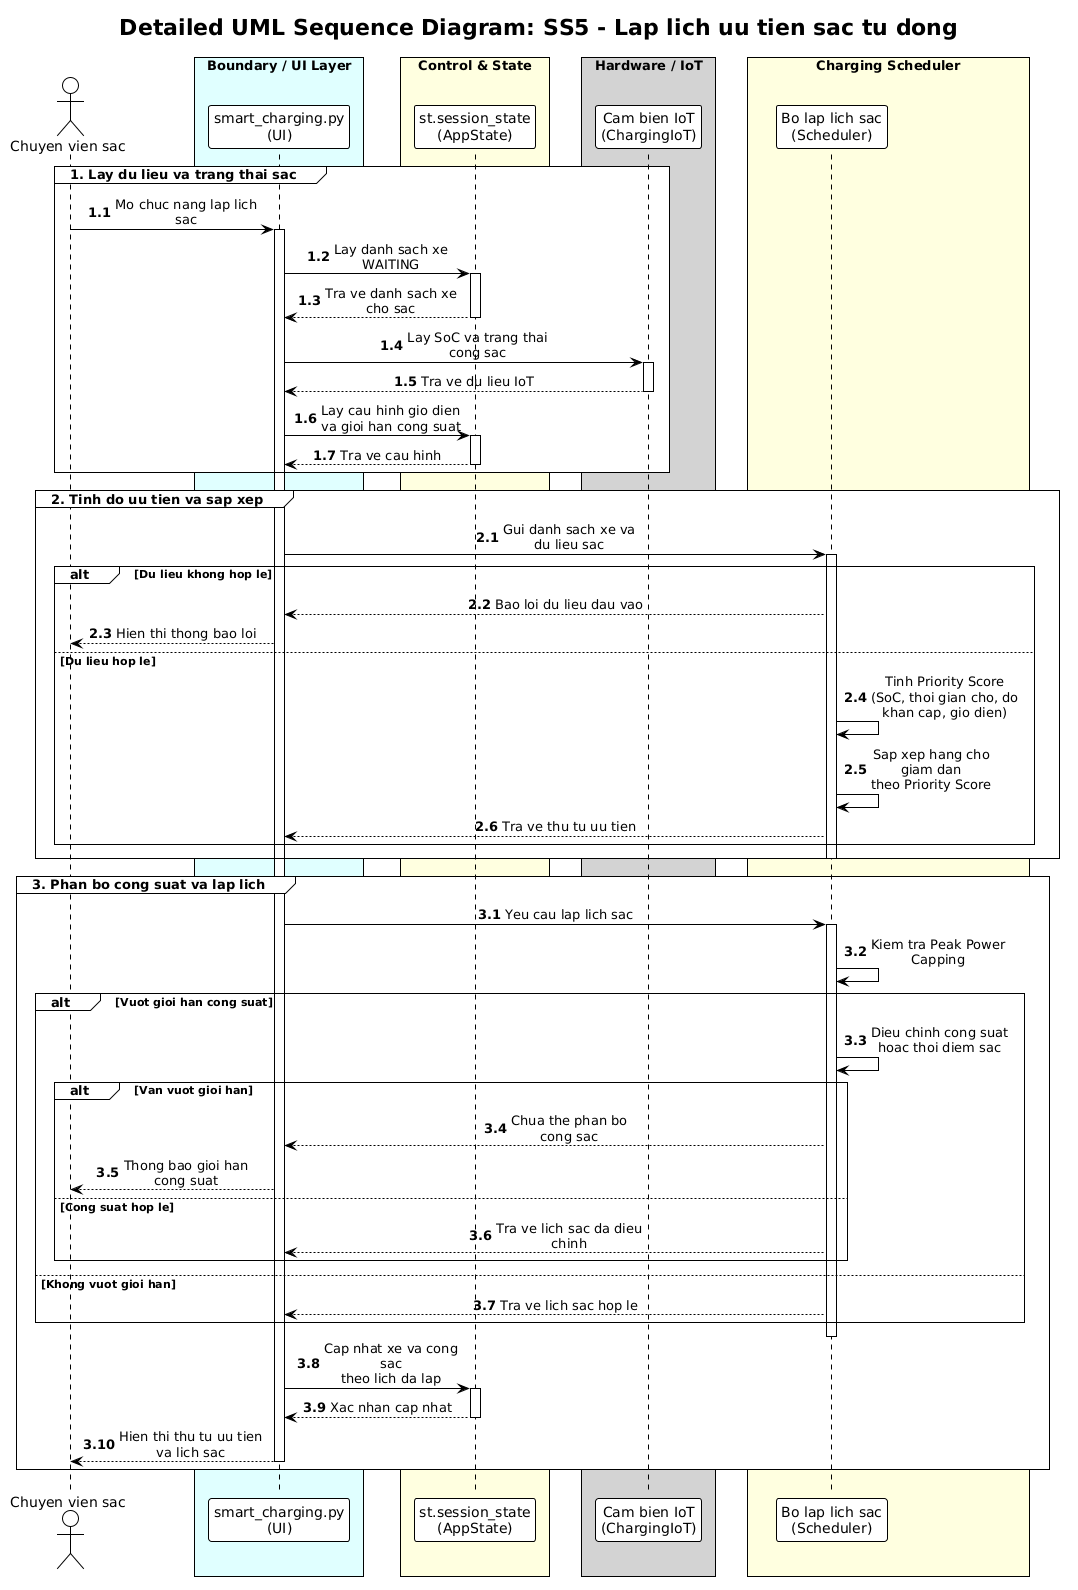
\includegraphics[width=0.88\textwidth]{Use-case detail-scenario/SS5/Sequence diagrams/UC_SS5_01_DuongDangKhoa_sequence.png}
    \caption{Sơ đồ Tuần tự Chi tiết -- UC\_SS5\_01 (Lập lịch ưu tiên sạc tự động)}
    \label{fig:seq-ss5-01}
\end{figure}

\subsubsection{UC\_SS5\_02: Giám sát hàng đợi sạc \& Phí chiếm dụng}
\paragraph{Mô tả nghiệp vụ:} Khi xe sạc đầy 100\%, hệ thống ngắt sạc và gửi thông báo cho sinh viên kèm thời gian ân hạn 15 phút. Nếu quá 15 phút xe chưa được rút, hệ thống bắt đầu tính phí phạt chiếm dụng trụ sạc 10.000đ/15 phút.
\begin{figure}[H]
    \centering
    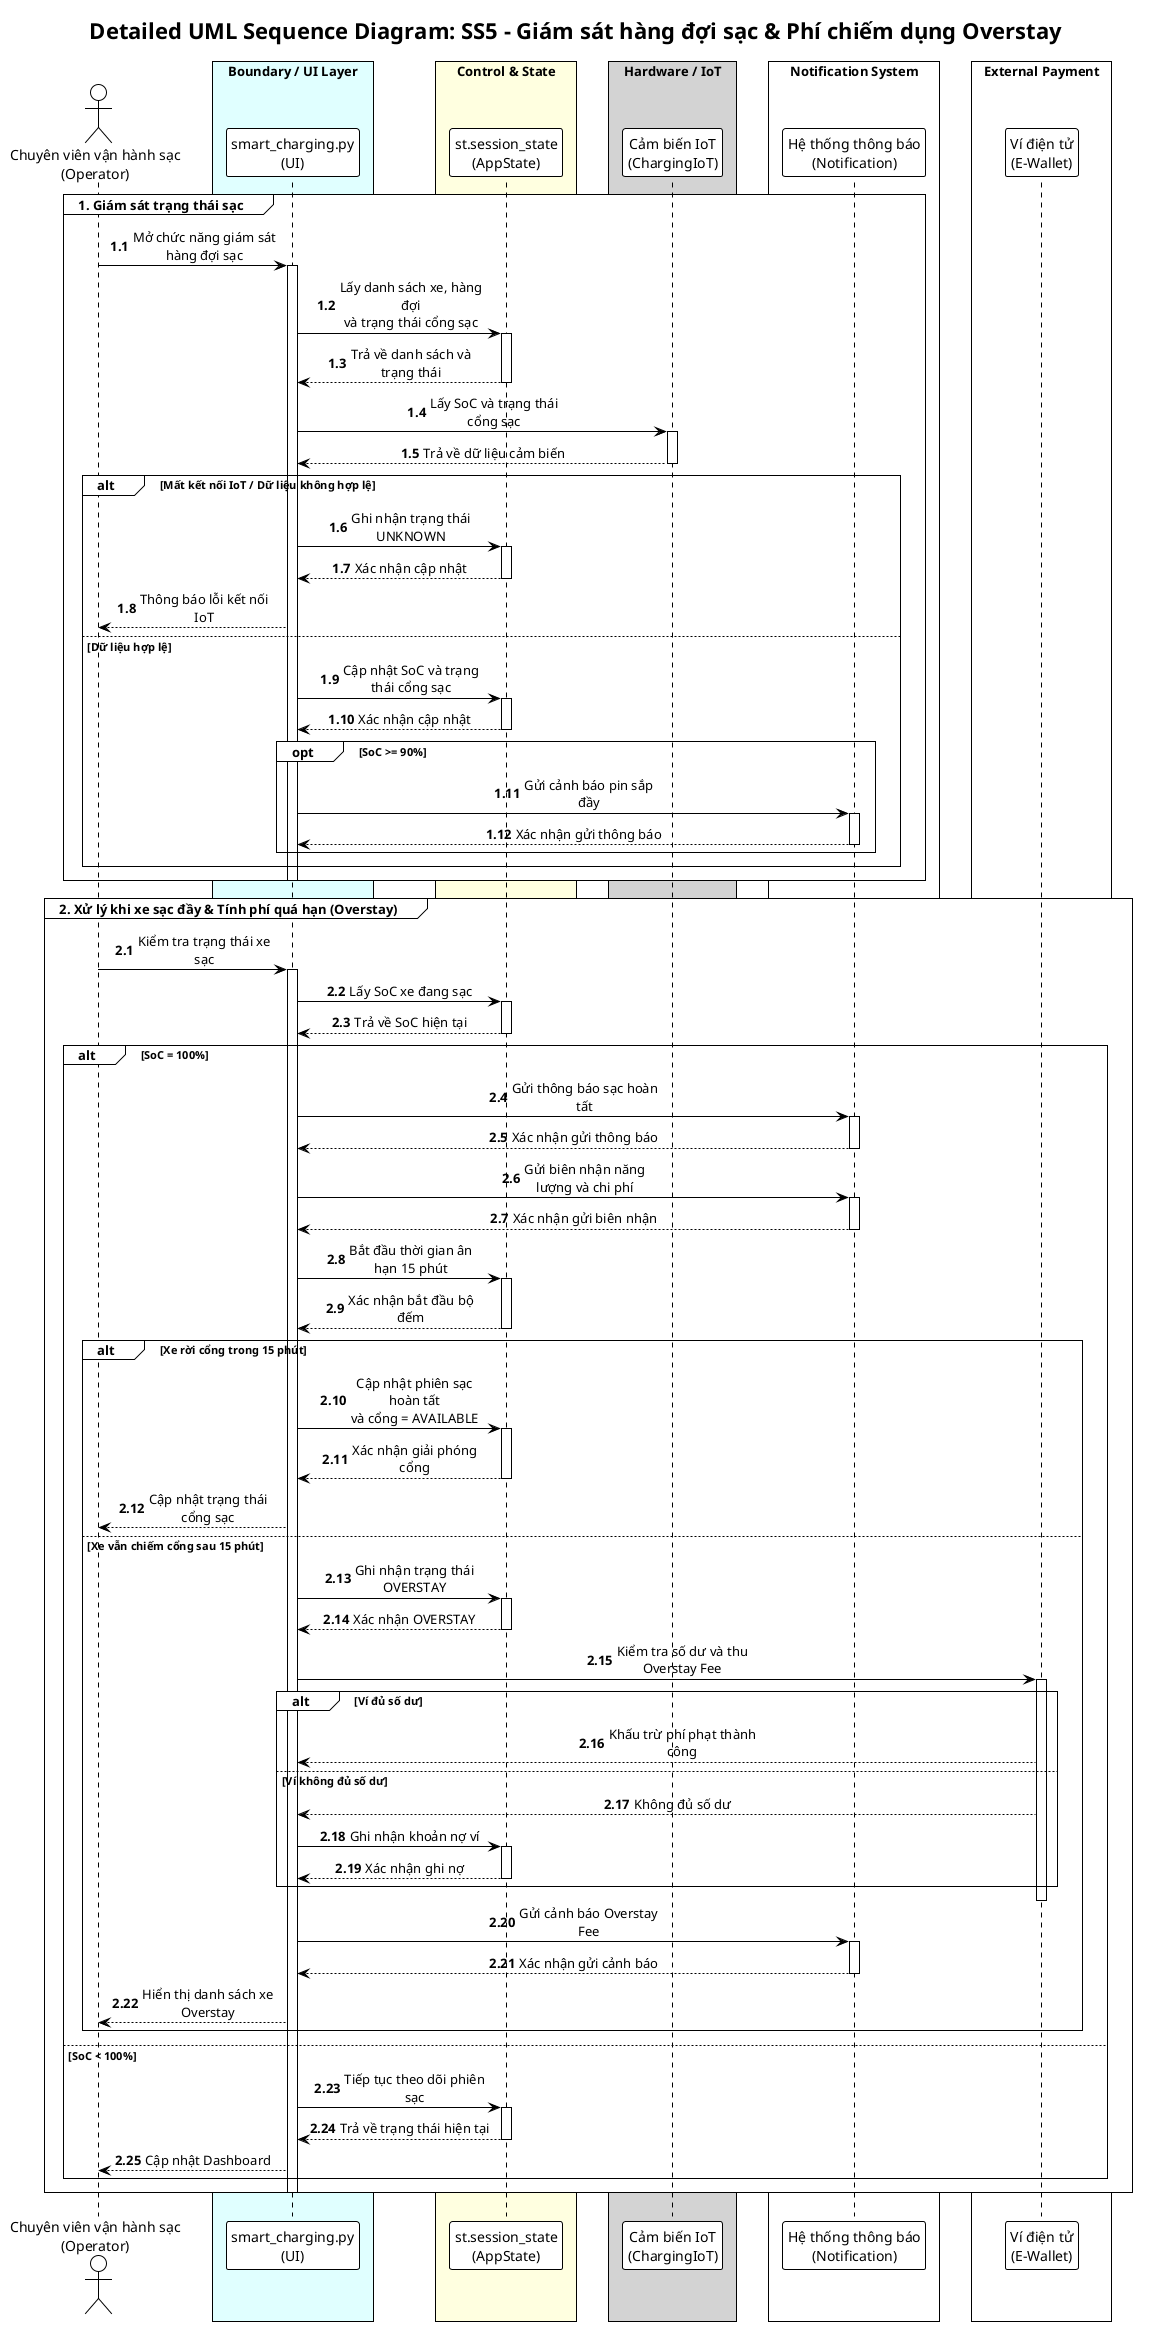
\includegraphics[width=0.88\textwidth]{Use-case detail-scenario/SS5/Sequence diagrams/UC_SS5_02_DuongDangKhoa_sequence.png}
    \caption{Sơ đồ Tuần tự Chi tiết -- UC\_SS5\_02 (Giám sát hàng đợi sạc \& Phí chiếm dụng)}
    \label{fig:seq-ss5-02}
\end{figure}

% ------------------------------------------------------------
% 2.6 SS6 - Hoàng Văn Tấn
% ------------------------------------------------------------
\subsection{Phân hệ SS6: Mô phỏng What-if Nhu cầu (Hoàng Văn Tấn)}

\subsubsection{UC\_SS6\_01: Mô phỏng đợt tăng đột biến hành khách Metro (Metro Surge)}
\paragraph{Mô tả nghiệp vụ:} Chuyên viên quy hoạch thiết lập tham số đợt xả khách Metro tại Ga Suối Tiên, động cơ mô phỏng \texttt{HubEventSimulator} tính toán áp lực thiếu xe và đề xuất lượng xe cần điều phối bù.
\begin{figure}[H]
    \centering
    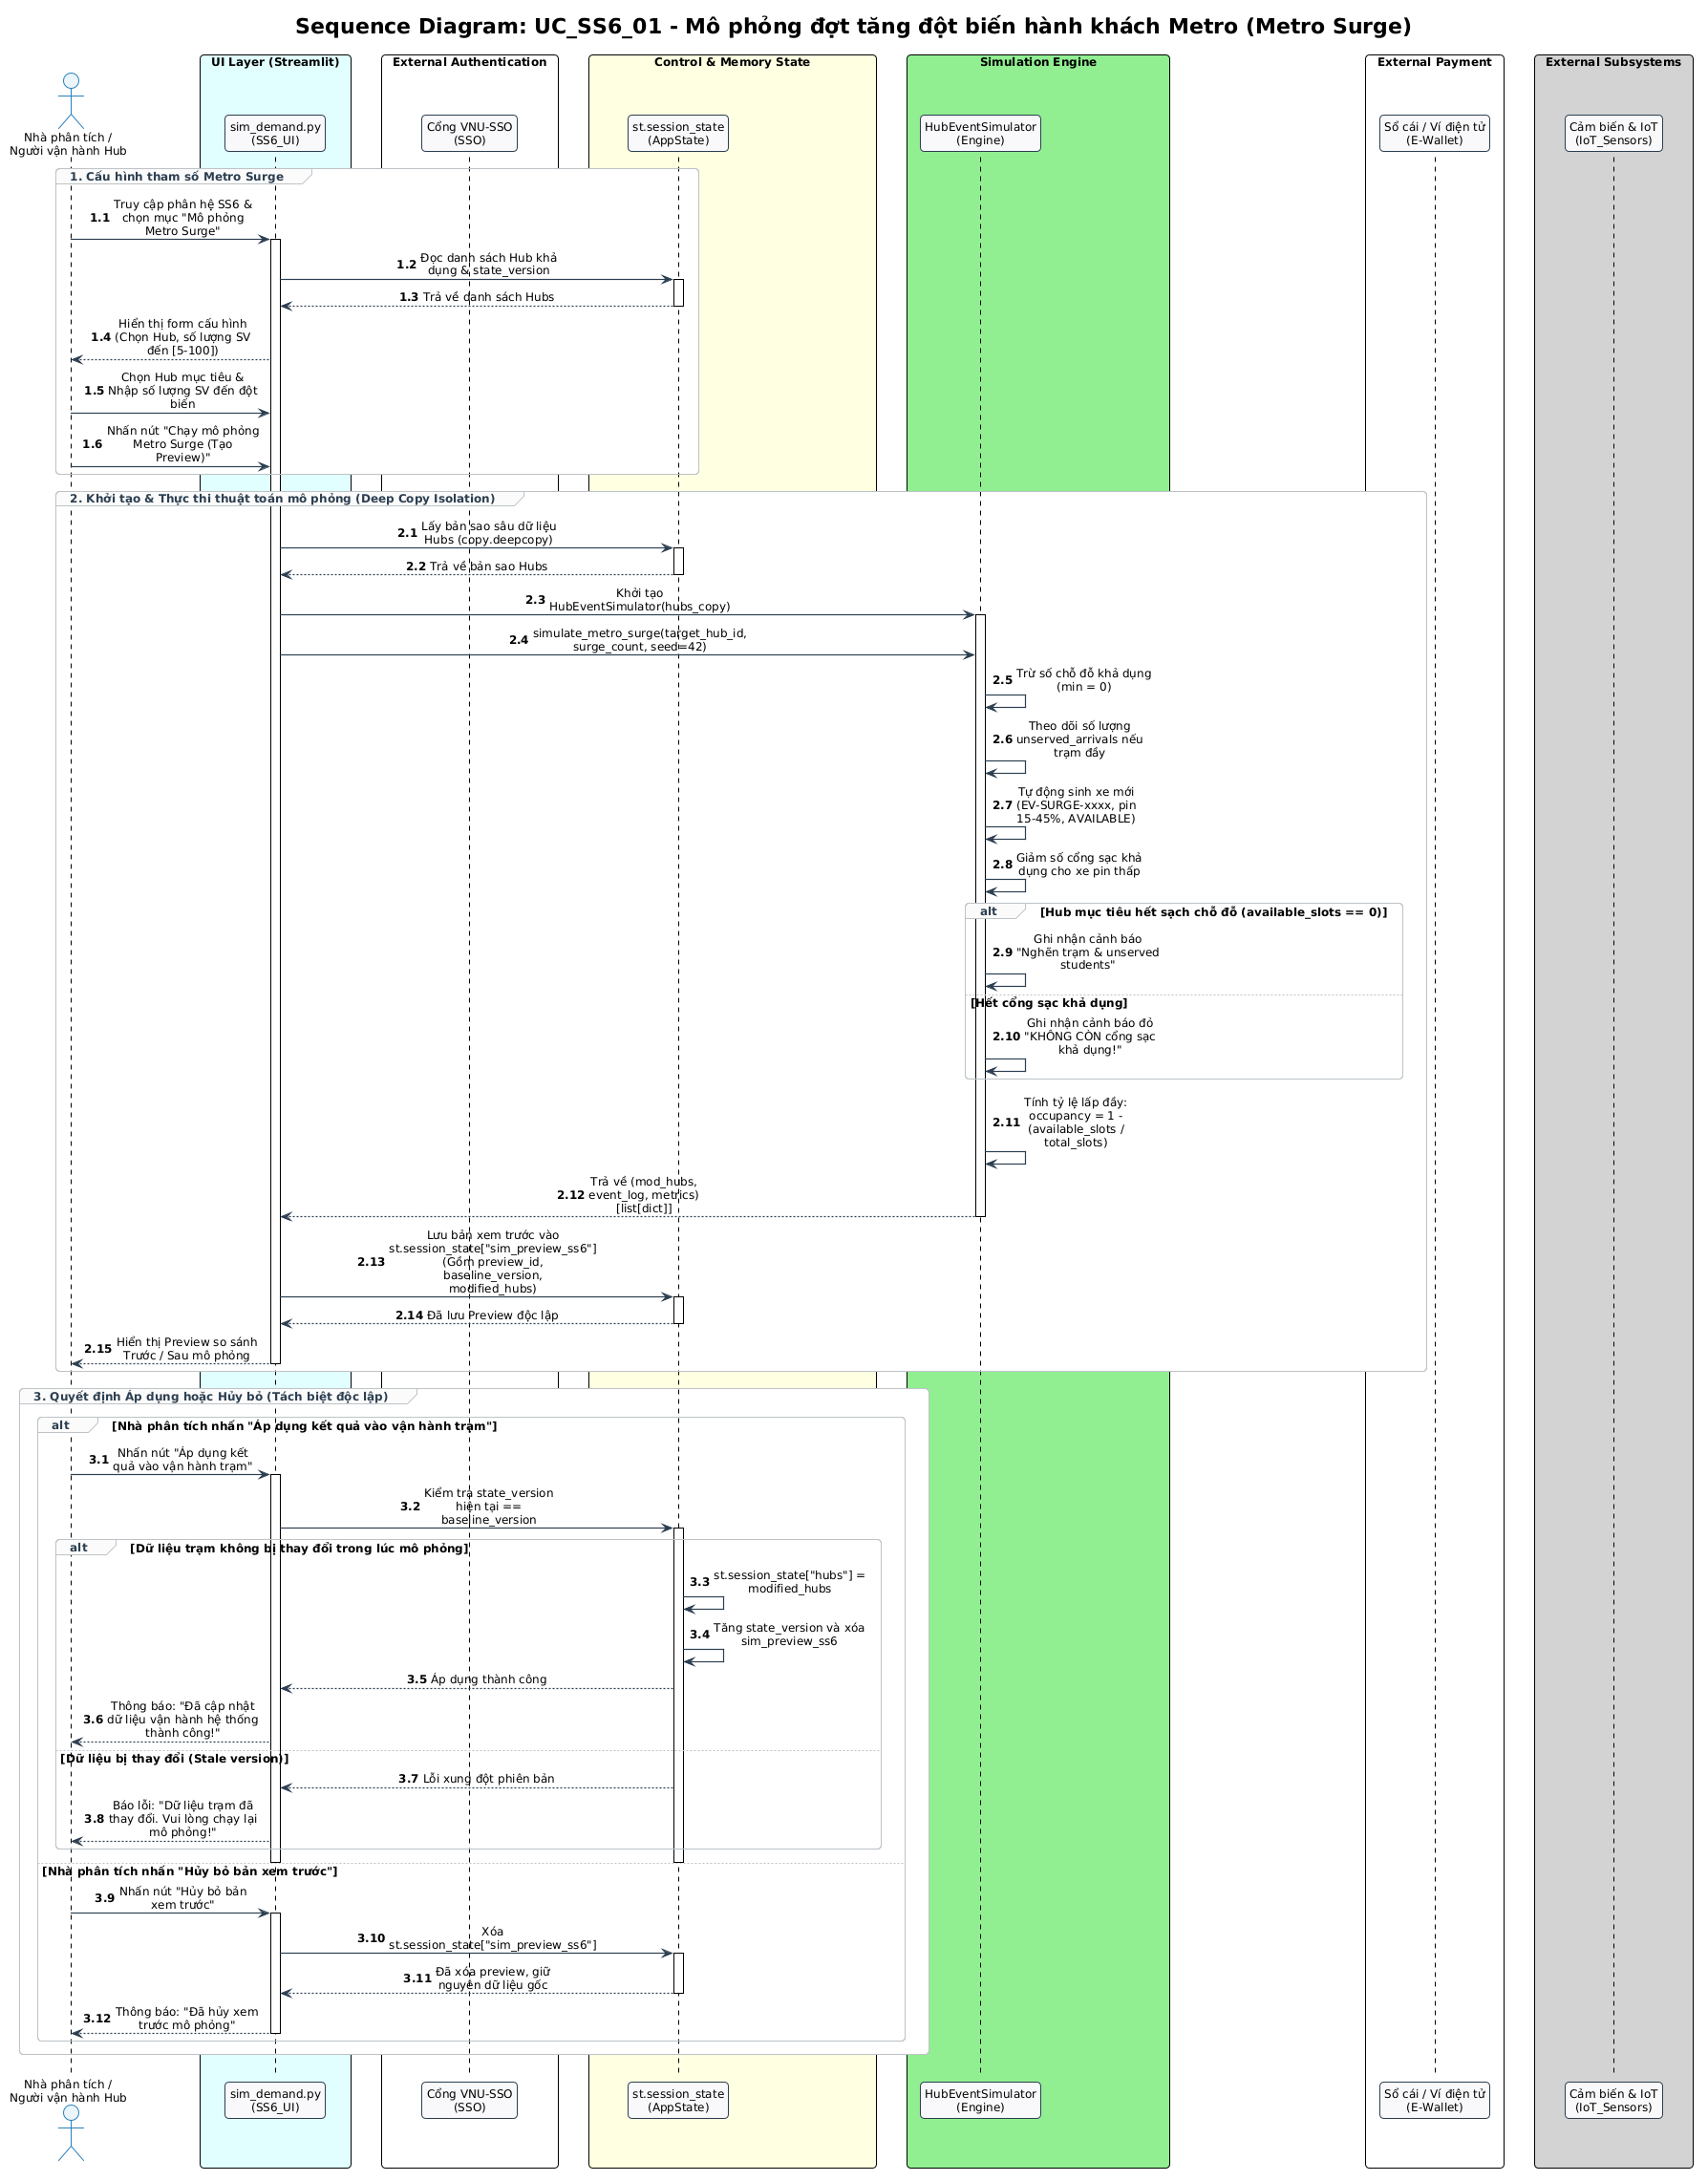
\includegraphics[width=0.88\textwidth]{Use-case detail-scenario/SS6/Sequence diagrams/UC_SS6_01_HoangVanTan_sequence.png}
    \caption{Sơ đồ Tuần tự Chi tiết -- UC\_SS6\_01 (Mô phỏng đợt tăng đột biến Metro Surge)}
    \label{fig:seq-ss6-01}
\end{figure}

\subsubsection{UC\_SS6\_02: Dự báo nhu cầu theo giờ \& Phân tích hàng đợi}
\paragraph{Mô tả nghiệp vụ:} Sử dụng dữ liệu chuỗi thời gian phân tích xác suất hành khách đổ về từng trạm Hub theo từng khung giờ trong ngày, đánh giá thời gian chờ và tỷ lệ đáp ứng phương tiện.
\begin{figure}[H]
    \centering
    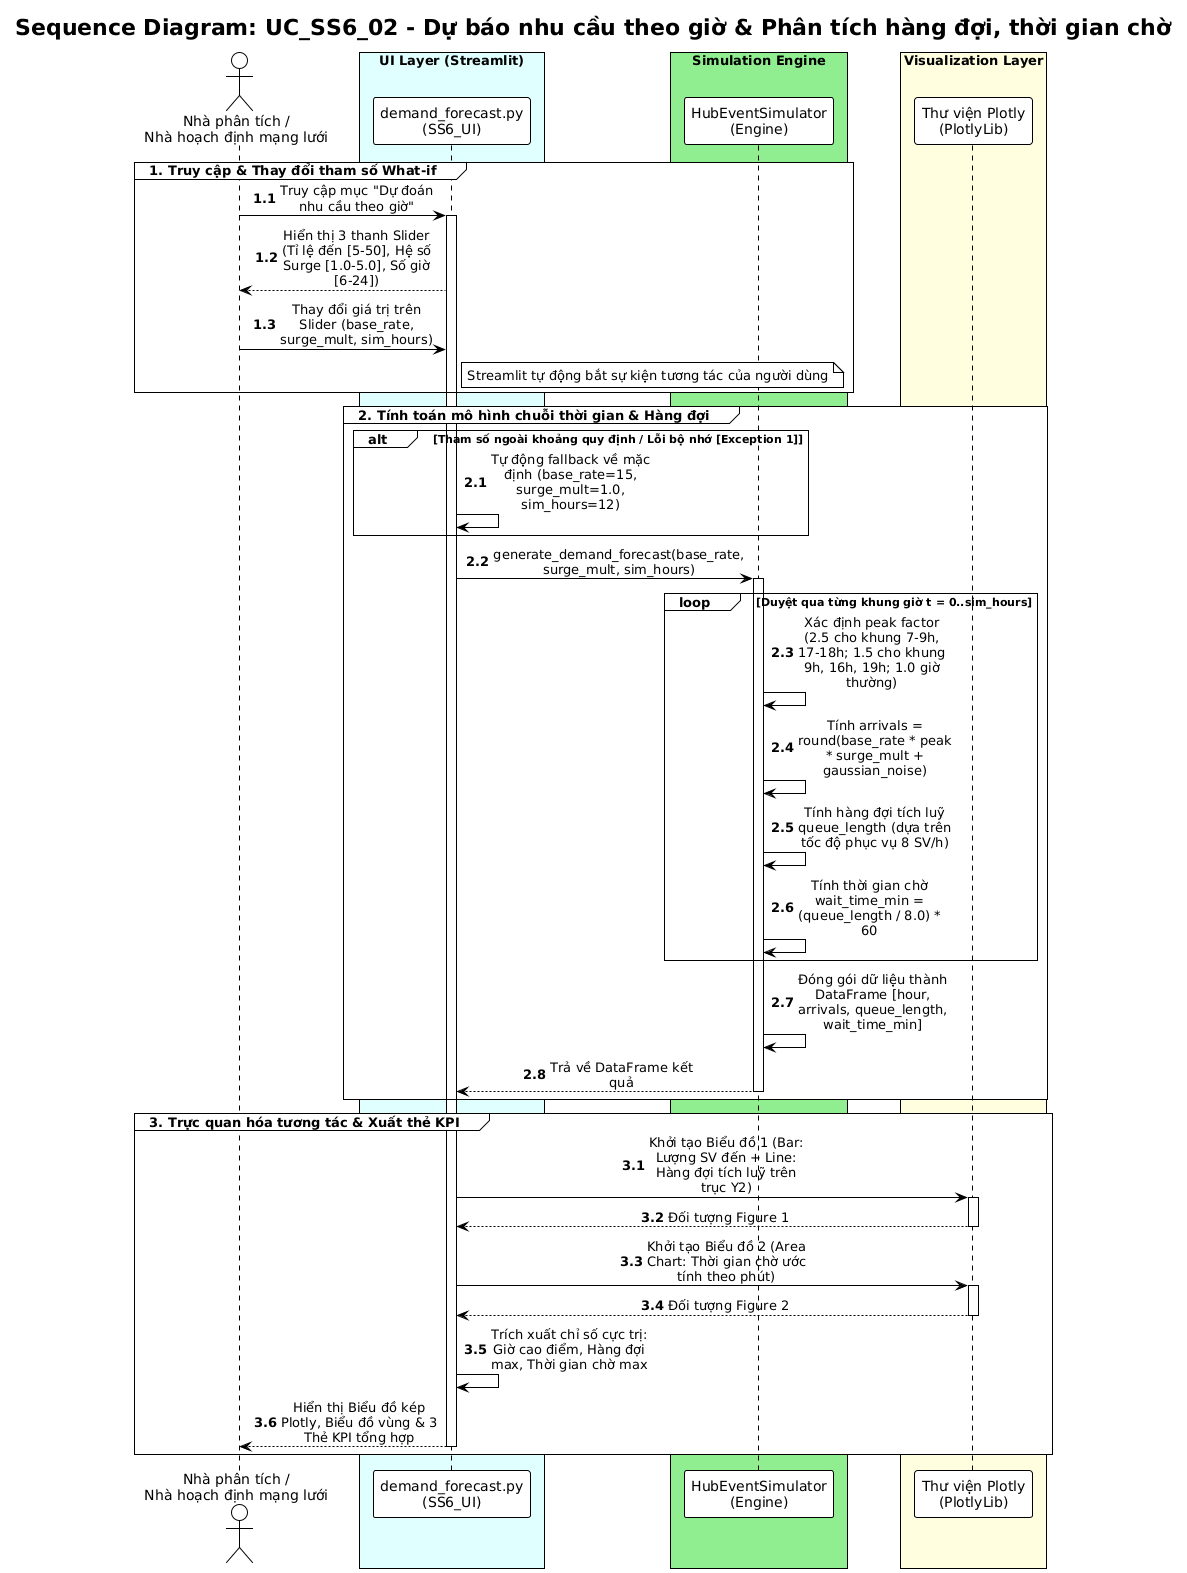
\includegraphics[width=0.88\textwidth]{Use-case detail-scenario/SS6/Sequence diagrams/UC_SS6_02_HoangVanTan_sequence.png}
    \caption{Sơ đồ Tuần tự Chi tiết -- UC\_SS6\_02 (Dự báo nhu cầu theo giờ \& Phân tích hàng đợi)}
    \label{fig:seq-ss6-02}
\end{figure}

% ------------------------------------------------------------
% 2.7 SS7 - Nguyễn Trung Nguyên
% ------------------------------------------------------------
\subsection{Phân hệ SS7: Mô phỏng What-if Hạ tầng (Nguyễn Trung Nguyên)}

\subsubsection{UC\_SS7\_01: Mô phỏng sự cố mất điện / lỗi cổng sạc}
\paragraph{Mô tả nghiệp vụ:} Kỹ thuật viên kích hoạt giả lập mất điện lưới tại Hub, hệ thống tự động cách ly các trụ sạc, chuyển sang nguồn UPS dự phòng cho cảm biến và cảnh báo dừng tiếp nhận đặt chỗ.
\begin{figure}[H]
    \centering
    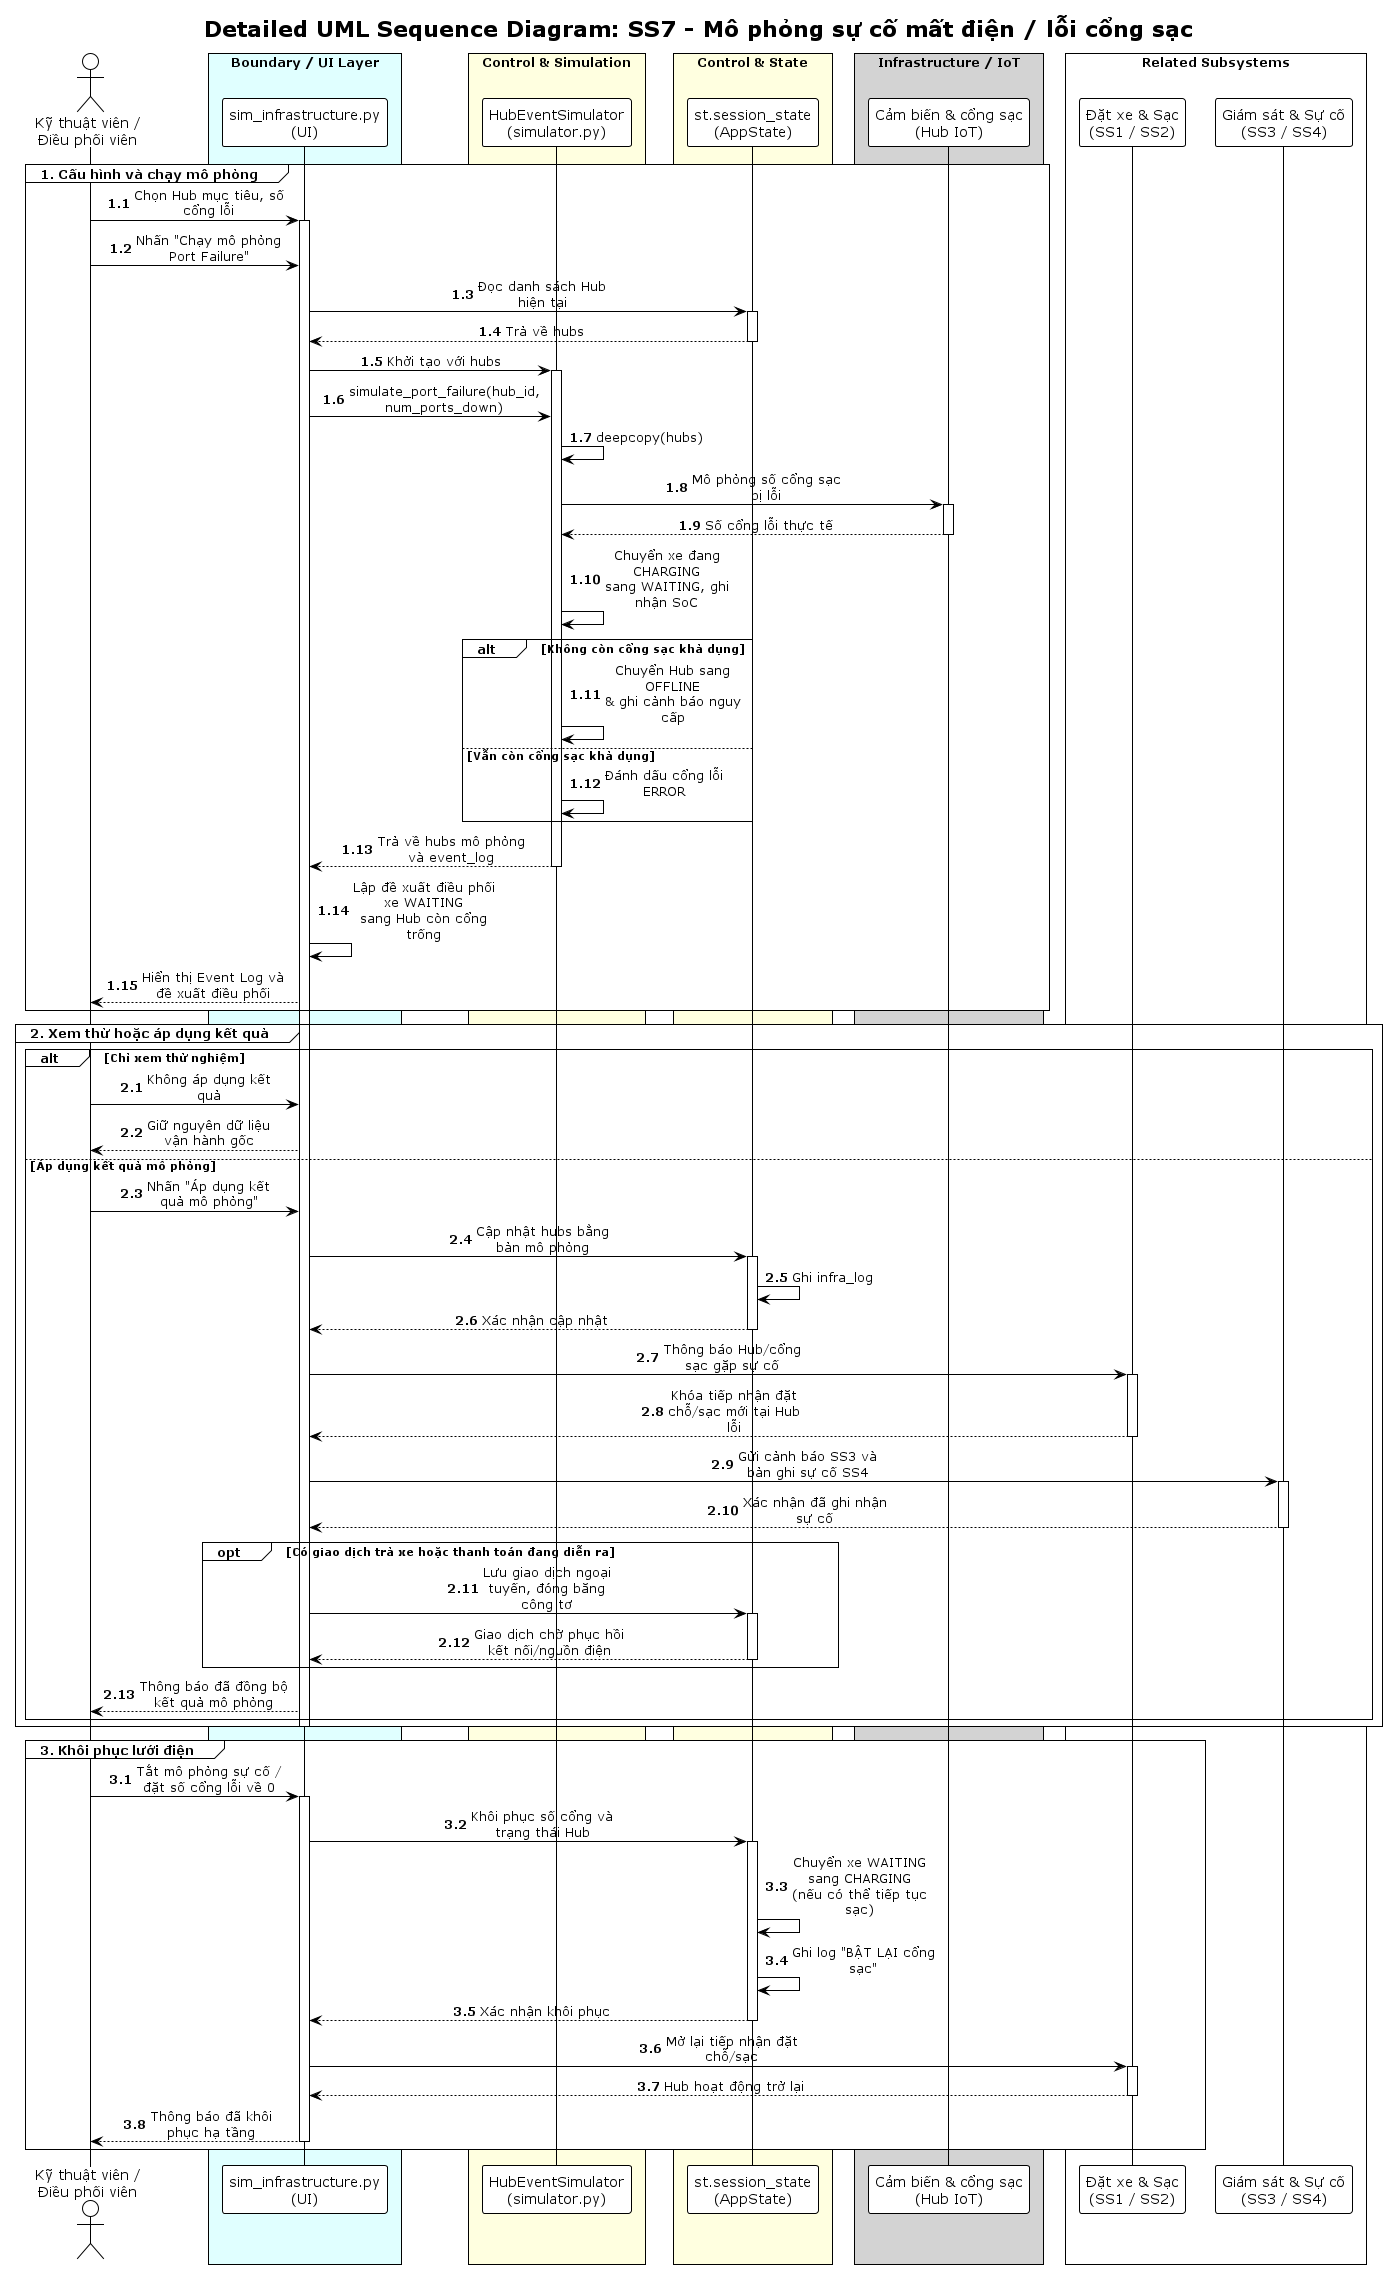
\includegraphics[width=0.88\textwidth]{Use-case detail-scenario/SS7/Sequence diagrams/UC_SS7_01_NguyenTrungNguyen_sequence.png}
    \caption{Sơ đồ Tuần tự Chi tiết -- UC\_SS7\_01 (Mô phỏng sự cố mất điện / lỗi trụ sạc)}
    \label{fig:seq-ss7-01}
\end{figure}

\subsubsection{UC\_SS7\_02: Tự động phát cảnh báo \& Gợi ý điều hướng 1-chạm}
\paragraph{Mô tả nghiệp vụ:} Quét ma trận khoảng cách không gian (Spatial Matrix), tìm 02 Hub lân cận còn slot trống, gửi thông báo điều hướng 1-chạm (One-tap Rerouting) đến sinh viên kèm ưu đãi miễn phí thêm 15 phút.
\begin{figure}[H]
    \centering
    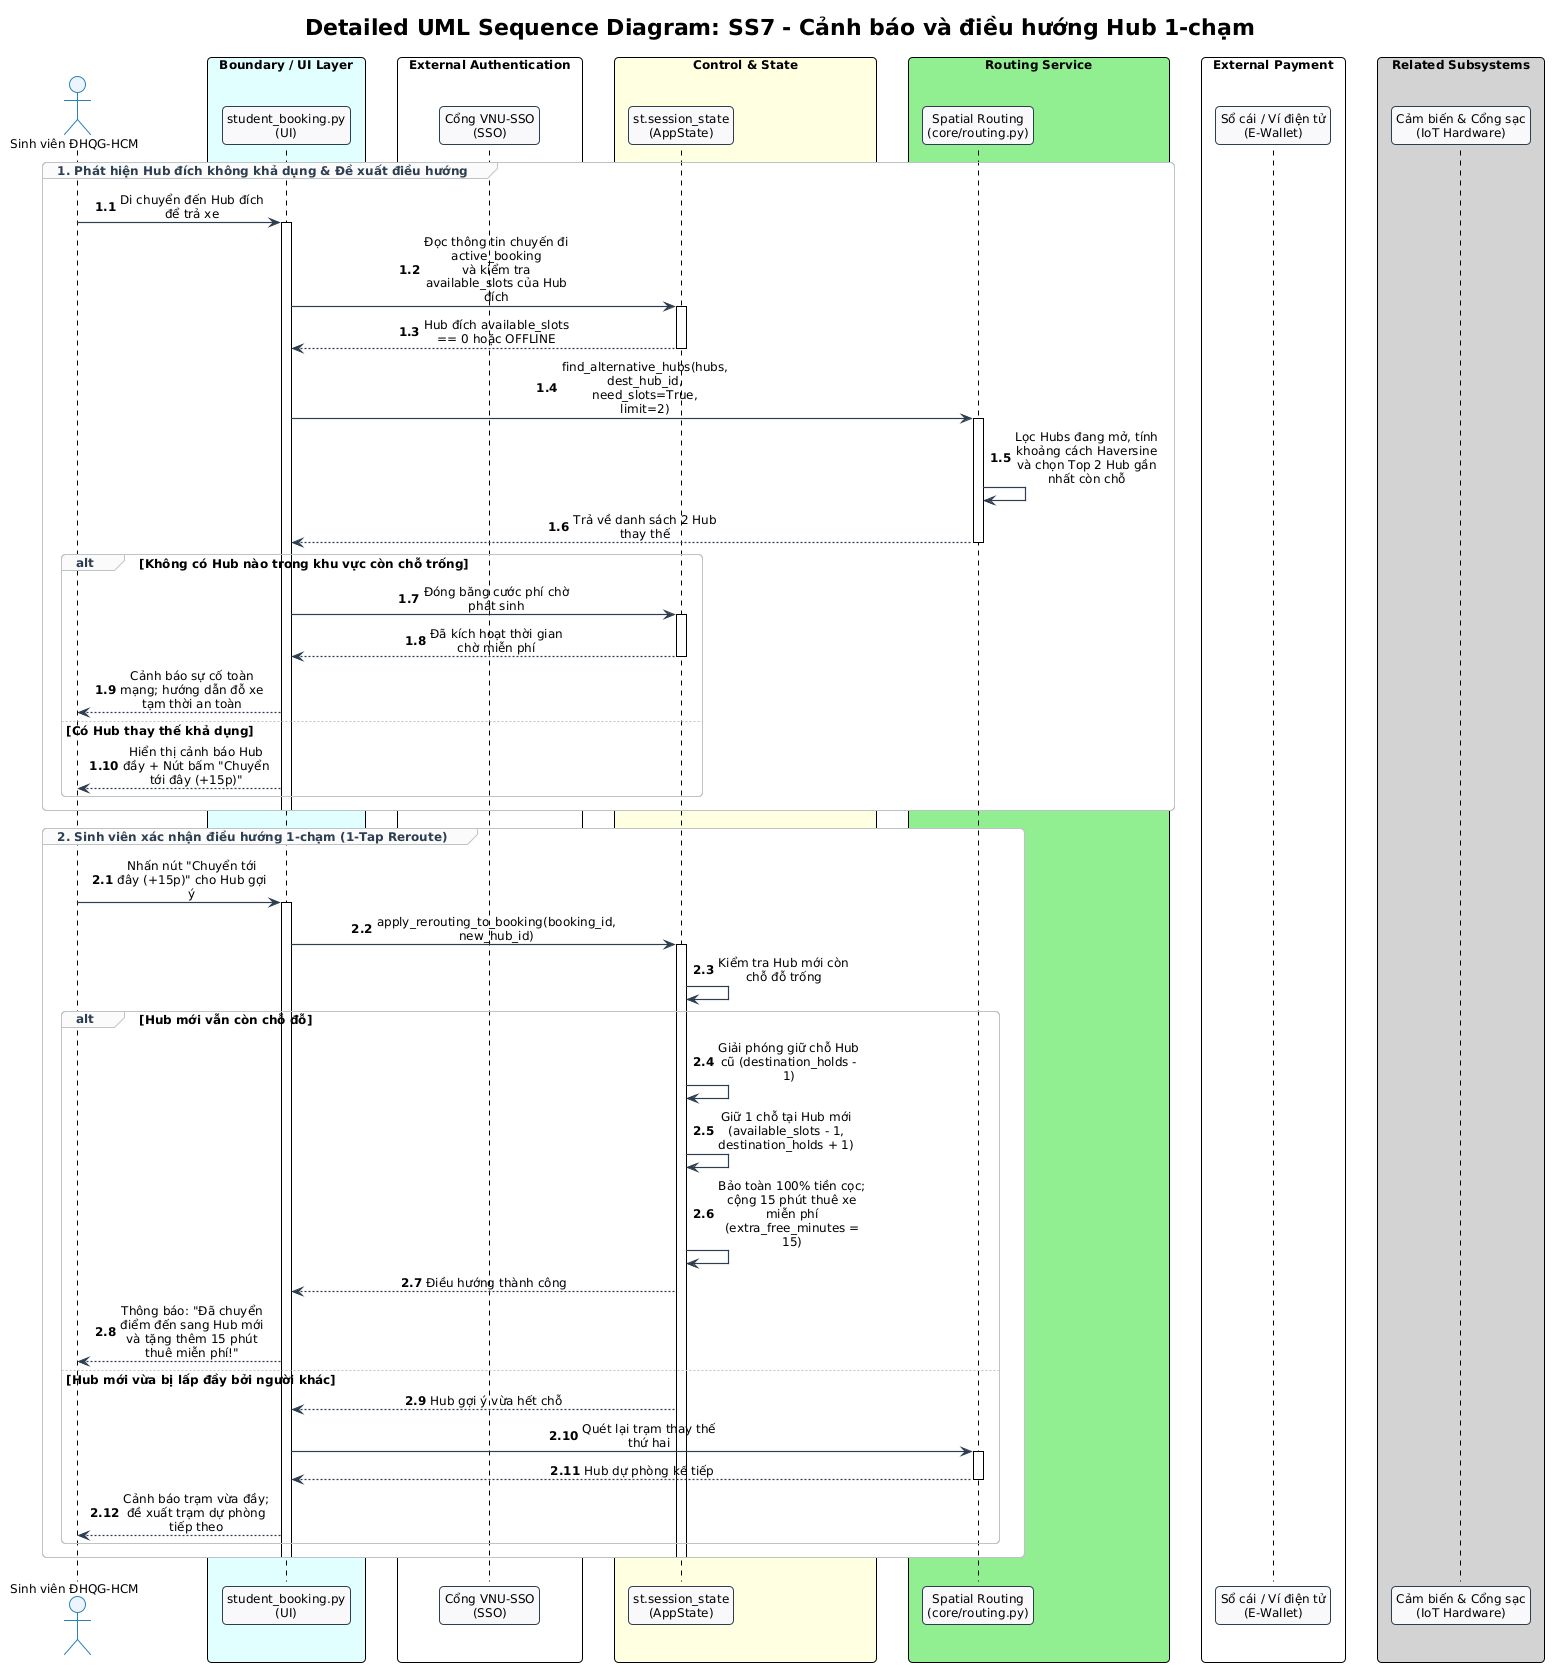
\includegraphics[width=0.88\textwidth]{Use-case detail-scenario/SS7/Sequence diagrams/UC_SS7_02_NguyenTrungNguyen_sequence.png}
    \caption{Sơ đồ Tuần tự Chi tiết -- UC\_SS7\_02 (Tự động phát cảnh báo \& Điều hướng 1-chạm)}
    \label{fig:seq-ss7-02}
\end{figure}
\newpage

% ============================================================
%       MỤC 3: SƠ ĐỒ HOẠT ĐỘNG - ACTIVITY DIAGRAMS (INDIVIDUAL WORK)
% ============================================================
\section{Sơ đồ Hoạt động -- Activity Diagrams (Individual Work)}

Sơ đồ hoạt động (Activity Diagram) thể hiện luồng điều khiển của quy trình nghiệp vụ với các làn bơi (\textbf{Swimlanes}) phân chia rõ ràng giữa \textbf{Người dùng (User / Actor)} và \textbf{Hệ thống (System / IoT / Backend)}.

\subsection*{Nguyên tắc Chuẩn hóa Luồng Nghiệp vụ (Alternative vs. Exception Flows)}
Toàn bộ 17 sơ đồ hoạt động phân làn (Swimlane Activity Diagrams) tuân thủ triệt để nguyên tắc phân định luồng rẽ nhánh:
\begin{itemize}[nosep]
    \item \textbf{Luồng Rẽ nhánh Nghiệp vụ (Alternative Flow):} Được biểu diễn qua các nút quyết định (\texttt{Decision Node}) với điều kiện bảo vệ (\texttt{Guard Condition}). Đây là các kịch bản nghiệp vụ hợp lệ có thể xảy ra trong thực tế (vd: số dư ví không đủ $\rightarrow$ gợi ý nạp tiền; hết xe khả dụng $\rightarrow$ đề xuất trạm lân cận; hết 15 phút ân hạn $\rightarrow$ áp dụng phí phạt giữ chỗ). Hệ thống luôn kiểm soát và điều hướng an toàn để kết thúc phiên.
    \item \textbf{Luồng Xử lý Ngoại lệ Kỹ thuật (Exception Flow):} Được bao bọc trong vùng ngắt có thể gián đoạn (\texttt{Interruptible Activity Region}) dẫn tới nút hủy (\texttt{Flow Final} hoặc \texttt{Activity Final}). Luồng này chỉ kích hoạt khi xảy ra sự cố kỹ thuật bất thường ngoài tầm kiểm soát nghiệp vụ (vd: mất kết nối internet/CSDL, cổng sạc quá nhiệt ngắt mạch, mất điện lưới diện rộng).
\end{itemize}

\begin{table}[H]
    \centering
    \small
    \renewcommand{\arraystretch}{1.2}
    \caption{Ma trận Phân loại Luồng Nghiệp vụ trong 17 Activity Diagrams}
    \label{tab:act-matrix}
    \begin{tabularx}{\textwidth}{|c|c|X|X|}
        \hline
        \textbf{Phân hệ} & \textbf{Mã UC} & \textbf{Luồng Rẽ Nhánh (Alternate Flow)} & \textbf{Luồng Ngoại Lệ (Exception Flow)} \\
        \hline
        SS1 & UC\_SS1\_01 & Nhập mã PIN thủ công thay vì quét QR & Số dư ví không đủ 50.000 VNĐ; quá 15p tự hủy \\
        SS1 & UC\_SS1\_02 & Trả xe khác Hub mượn (1-chiều) & Pin dưới 20\% phạt sạc; chốt khóa Hub báo đầy \\
        SS1 & UC\_SS1\_03 & Sinh viên chủ động hủy qua ứng dụng & Lỗi timeout kết nối ví điện tử VNU \\
        \hline
        SS2 & UC\_SS2\_01 & Bổ sung giấy tờ xe qua xác minh thủ công & Biển số xe đã tồn tại trên hệ thống \\
        SS2 & UC\_SS2\_02 & Chỉ đỗ xe không sạc điện & Hết chỗ đỗ hoặc không có cổng sạc phù hợp \\
        SS2 & UC\_SS2\_03 & Nhận diện tự động qua camera ANPR & Thẻ RFID lỗi, nhập mã đặt chỗ dự phòng \\
        SS2 & UC\_SS2\_04 & Thanh toán qua ví điện tử nội bộ & Số dư ví không đủ, chuyển cổng VNPay \\
        \hline
        SS3 & UC\_SS3\_01 & Lọc hiển thị theo từng khu vực Hub & Mất tín hiệu cảm biến IoT quá 60 giây \\
        SS3 & UC\_SS3\_02 & Hệ thống tự động đẩy đề xuất lệnh sang SS4 & Người điều hành từ chối lệnh đề xuất \\
        \hline
        SS4 & UC\_SS4\_01 & Điều phối xe tải lớn vận chuyển hàng loạt & Lái xe điều phối báo tắc đường trễ giờ \\
        SS4 & UC\_SS4\_02 & Kỹ thuật viên sửa chữa tại chỗ thành công & Xe hư nặng kéo về xưởng bảo trì trung tâm \\
        \hline
        SS5 & UC\_SS5\_01 & Ưu tiên xe pin thấp dưới 20\% sạc trước & Quá tải công suất trạm, giảm dòng sạc an toàn \\
        SS5 & UC\_SS5\_02 & Sinh viên di chuyển xe trong 15p ân hạn & Quá 15p tính phí chiếm dụng 10.000đ/15p \\
        \hline
        SS6 & UC\_SS6\_01 & Điều chỉnh tham số Metro tăng 200\% & Dữ liệu lịch sử tuyến Metro không khả dụng \\
        SS6 & UC\_SS6\_02 & Xuất báo cáo phân tích định dạng PDF & Thời gian chờ tính toán vượt ngưỡng an toàn \\
        \hline
        SS7 & UC\_SS7\_01 & Chuyển tải sang máy phát điện phụ trợ & Trạm sạc chập điện ngắt toàn bộ trạm \\
        SS7 & UC\_SS7\_02 & Sinh viên chấp nhận gợi ý Hub lân cận & Sinh viên từ chối, hủy phiên và hoàn cọc \\
        \hline
    \end{tabularx}
\end{table}

\subsection{Phân hệ SS1: Đặt \& Quản lý Xe dùng chung (Nguyễn Thành Đạt)}

\subsubsection{UC\_SS1\_01: Đặt giữ chỗ \& Quét QR/PIN nhận xe}
\paragraph{Phân tích làn bơi (Swimlane):}
\begin{itemize}[nosep]
    \item \textbf{Làn bơi Sinh viên (Actor):} Mở app $\rightarrow$ Chọn Hub \& Xe $\rightarrow$ Xác nhận đặt cọc $\rightarrow$ Quét mã QR/PIN tại Hub.
    \item \textbf{Làn bơi Hệ thống (Backend/IoT):} Kiểm tra ví $\ge 50$k $\rightarrow$ Khóa xe 15p $\rightarrow$ Xác thực mã PIN/QR $\rightarrow$ Mở khóa vật lý $\rightarrow$ Chuyển \texttt{IN\_USE}.
\end{itemize}
\begin{figure}[H]
    \centering
    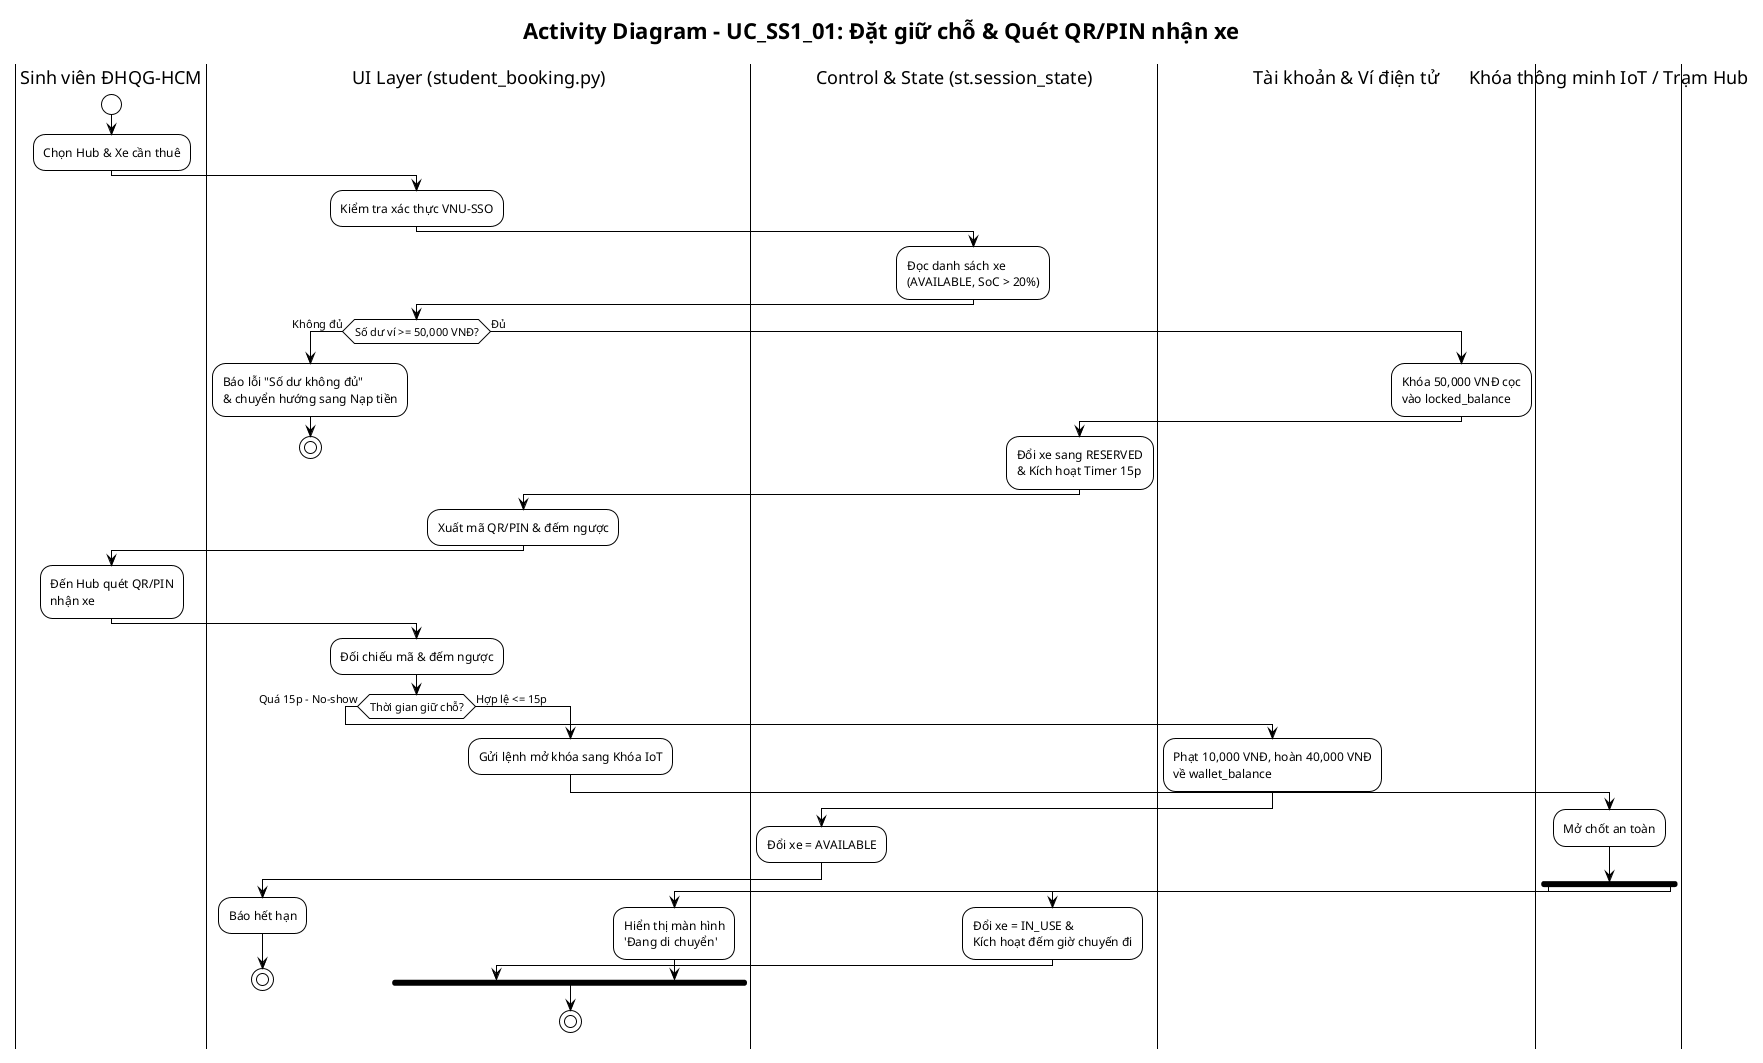
\includegraphics[width=0.92\textwidth]{Use-case detail-scenario/SS1/Activity diagrams/UC_SS1_01_NguyenThanhDat_activity.png}
    \caption{Sơ đồ Hoạt động Phân làn (Swimlane) -- UC\_SS1\_01}
    \label{fig:act-ss1-01}
\end{figure}

\subsubsection{UC\_SS1\_02: Trả xe 1-chiều \& Quyết toán ví điện tử}
\begin{figure}[H]
    \centering
    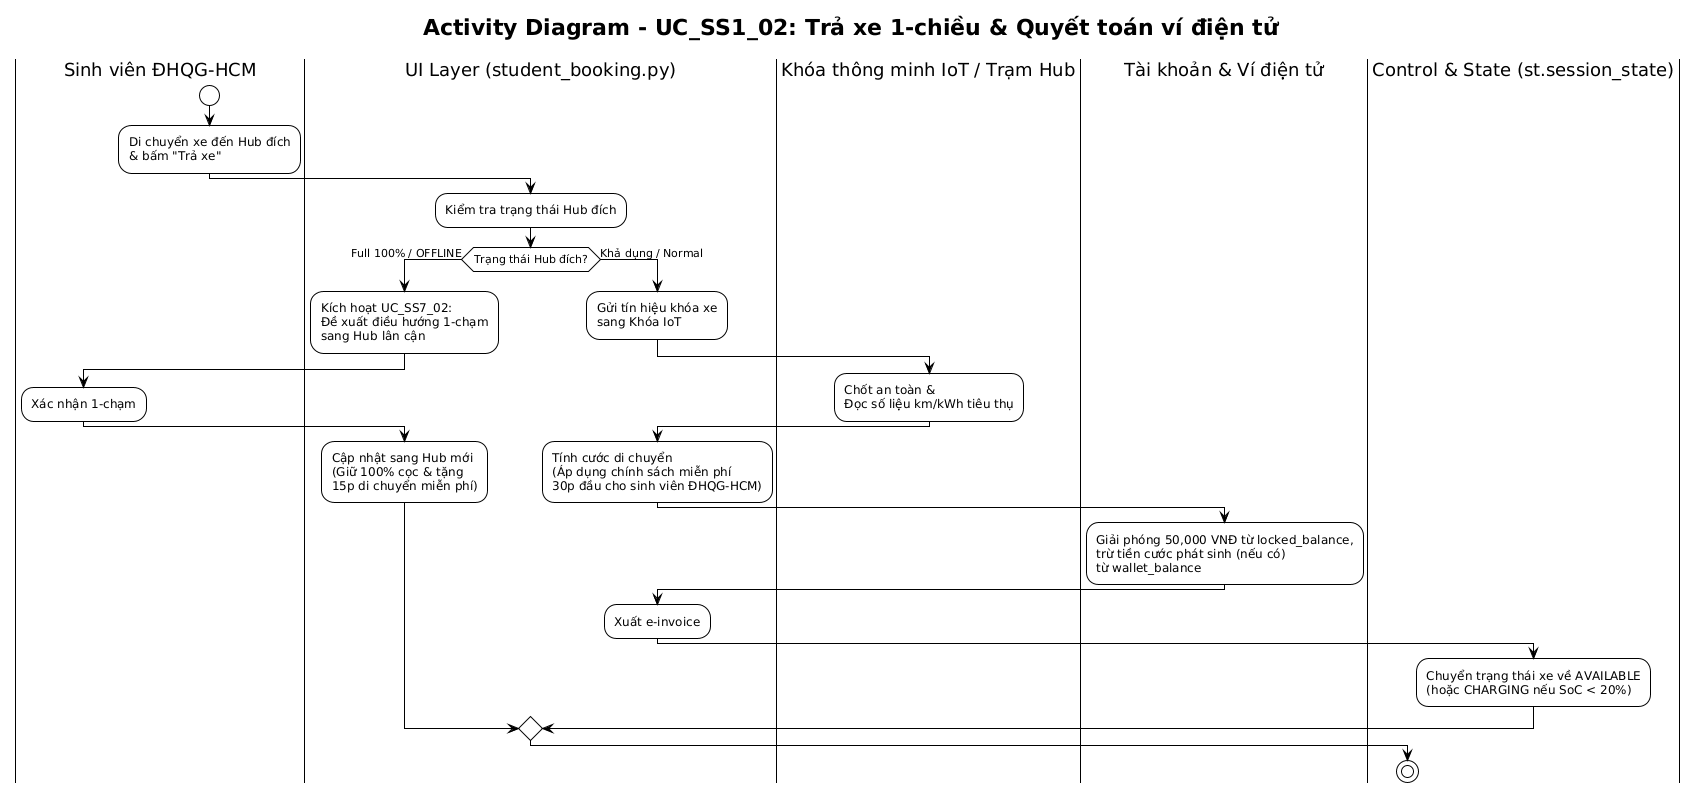
\includegraphics[width=0.92\textwidth]{Use-case detail-scenario/SS1/Activity diagrams/UC_SS1_02_NguyenThanhDat_activity.png}
    \caption{Sơ đồ Hoạt động Phân làn (Swimlane) -- UC\_SS1\_02}
    \label{fig:act-ss1-02}
\end{figure}

\subsubsection{UC\_SS1\_03: Hủy đặt xe \& Hoàn 100\% cọc}
\begin{figure}[H]
    \centering
    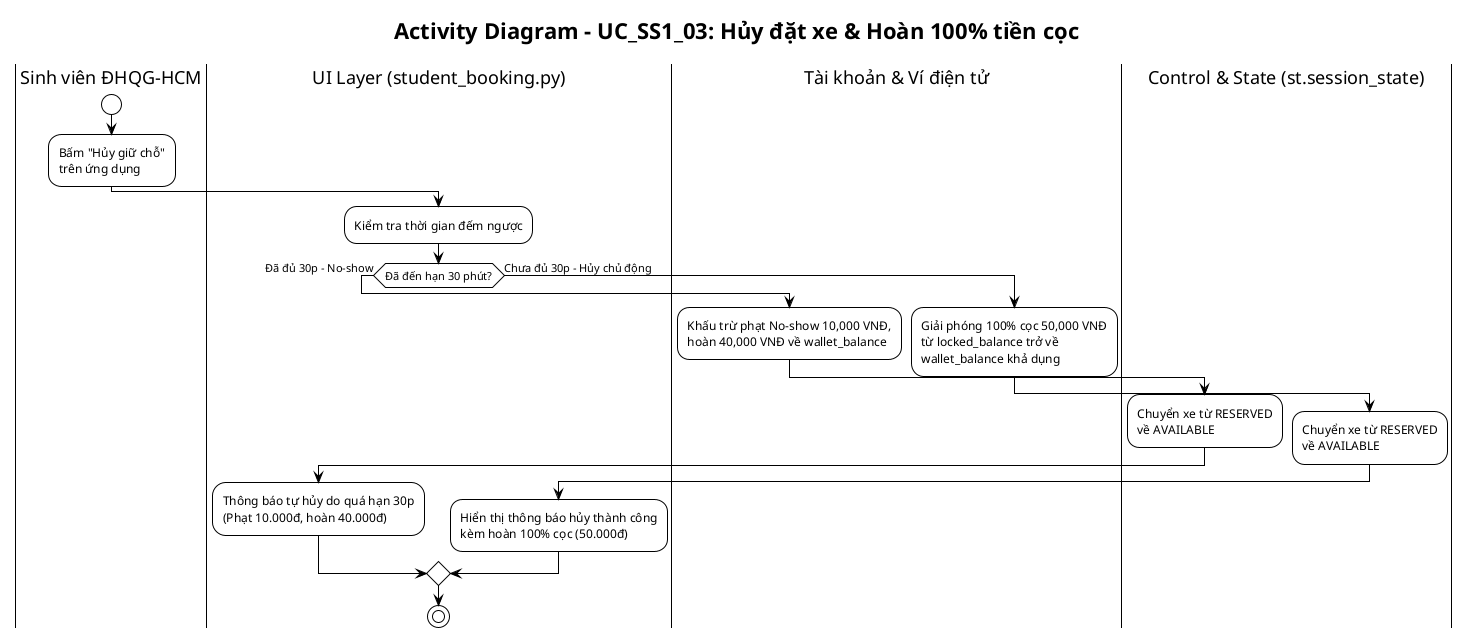
\includegraphics[width=0.92\textwidth]{Use-case detail-scenario/SS1/Activity diagrams/UC_SS1_03_NguyenThanhDat_activity.png}
    \caption{Sơ đồ Hoạt động Phân làn (Swimlane) -- UC\_SS1\_03}
    \label{fig:act-ss1-03}
\end{figure}

\subsection{Phân hệ SS2: Đăng ký Sạc \& Đỗ xe cá nhân (Nguyễn Anh Tài)}
\subsubsection{UC\_SS2\_01: Đăng ký xe EV cá nhân}
\begin{figure}[H]
    \centering
    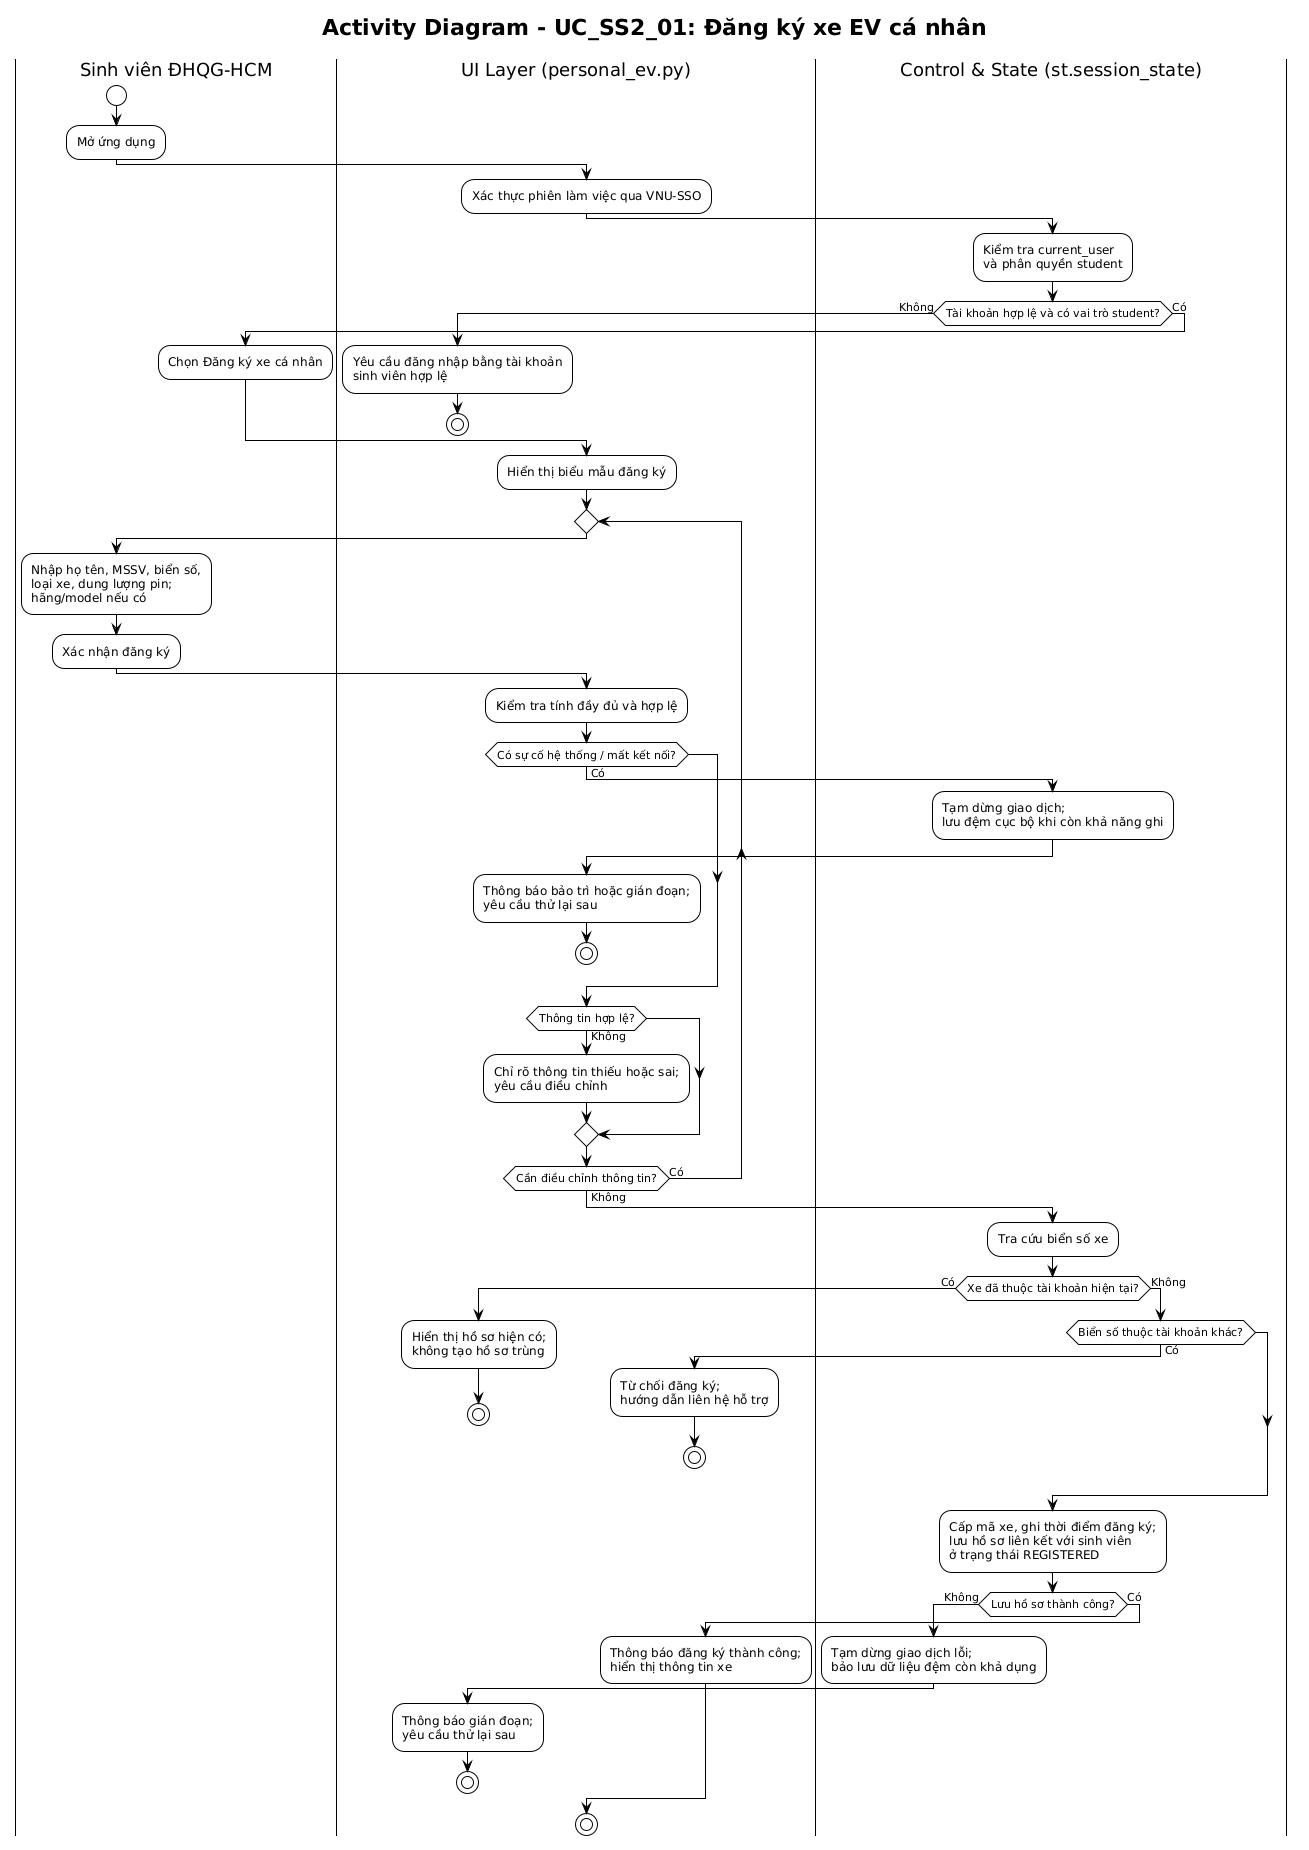
\includegraphics[width=0.92\textwidth]{Use-case detail-scenario/SS2/Activity diagrams/UC_SS2_01_NguyenAnhTai_activity.png}
    \caption{Sơ đồ Hoạt động Phân làn -- UC\_SS2\_01}
    \label{fig:act-ss2-01}
\end{figure}

\subsubsection{UC\_SS2\_02: Đặt chỗ đỗ và nhu cầu sạc xe EV cá nhân}
\begin{figure}[H]
    \centering
    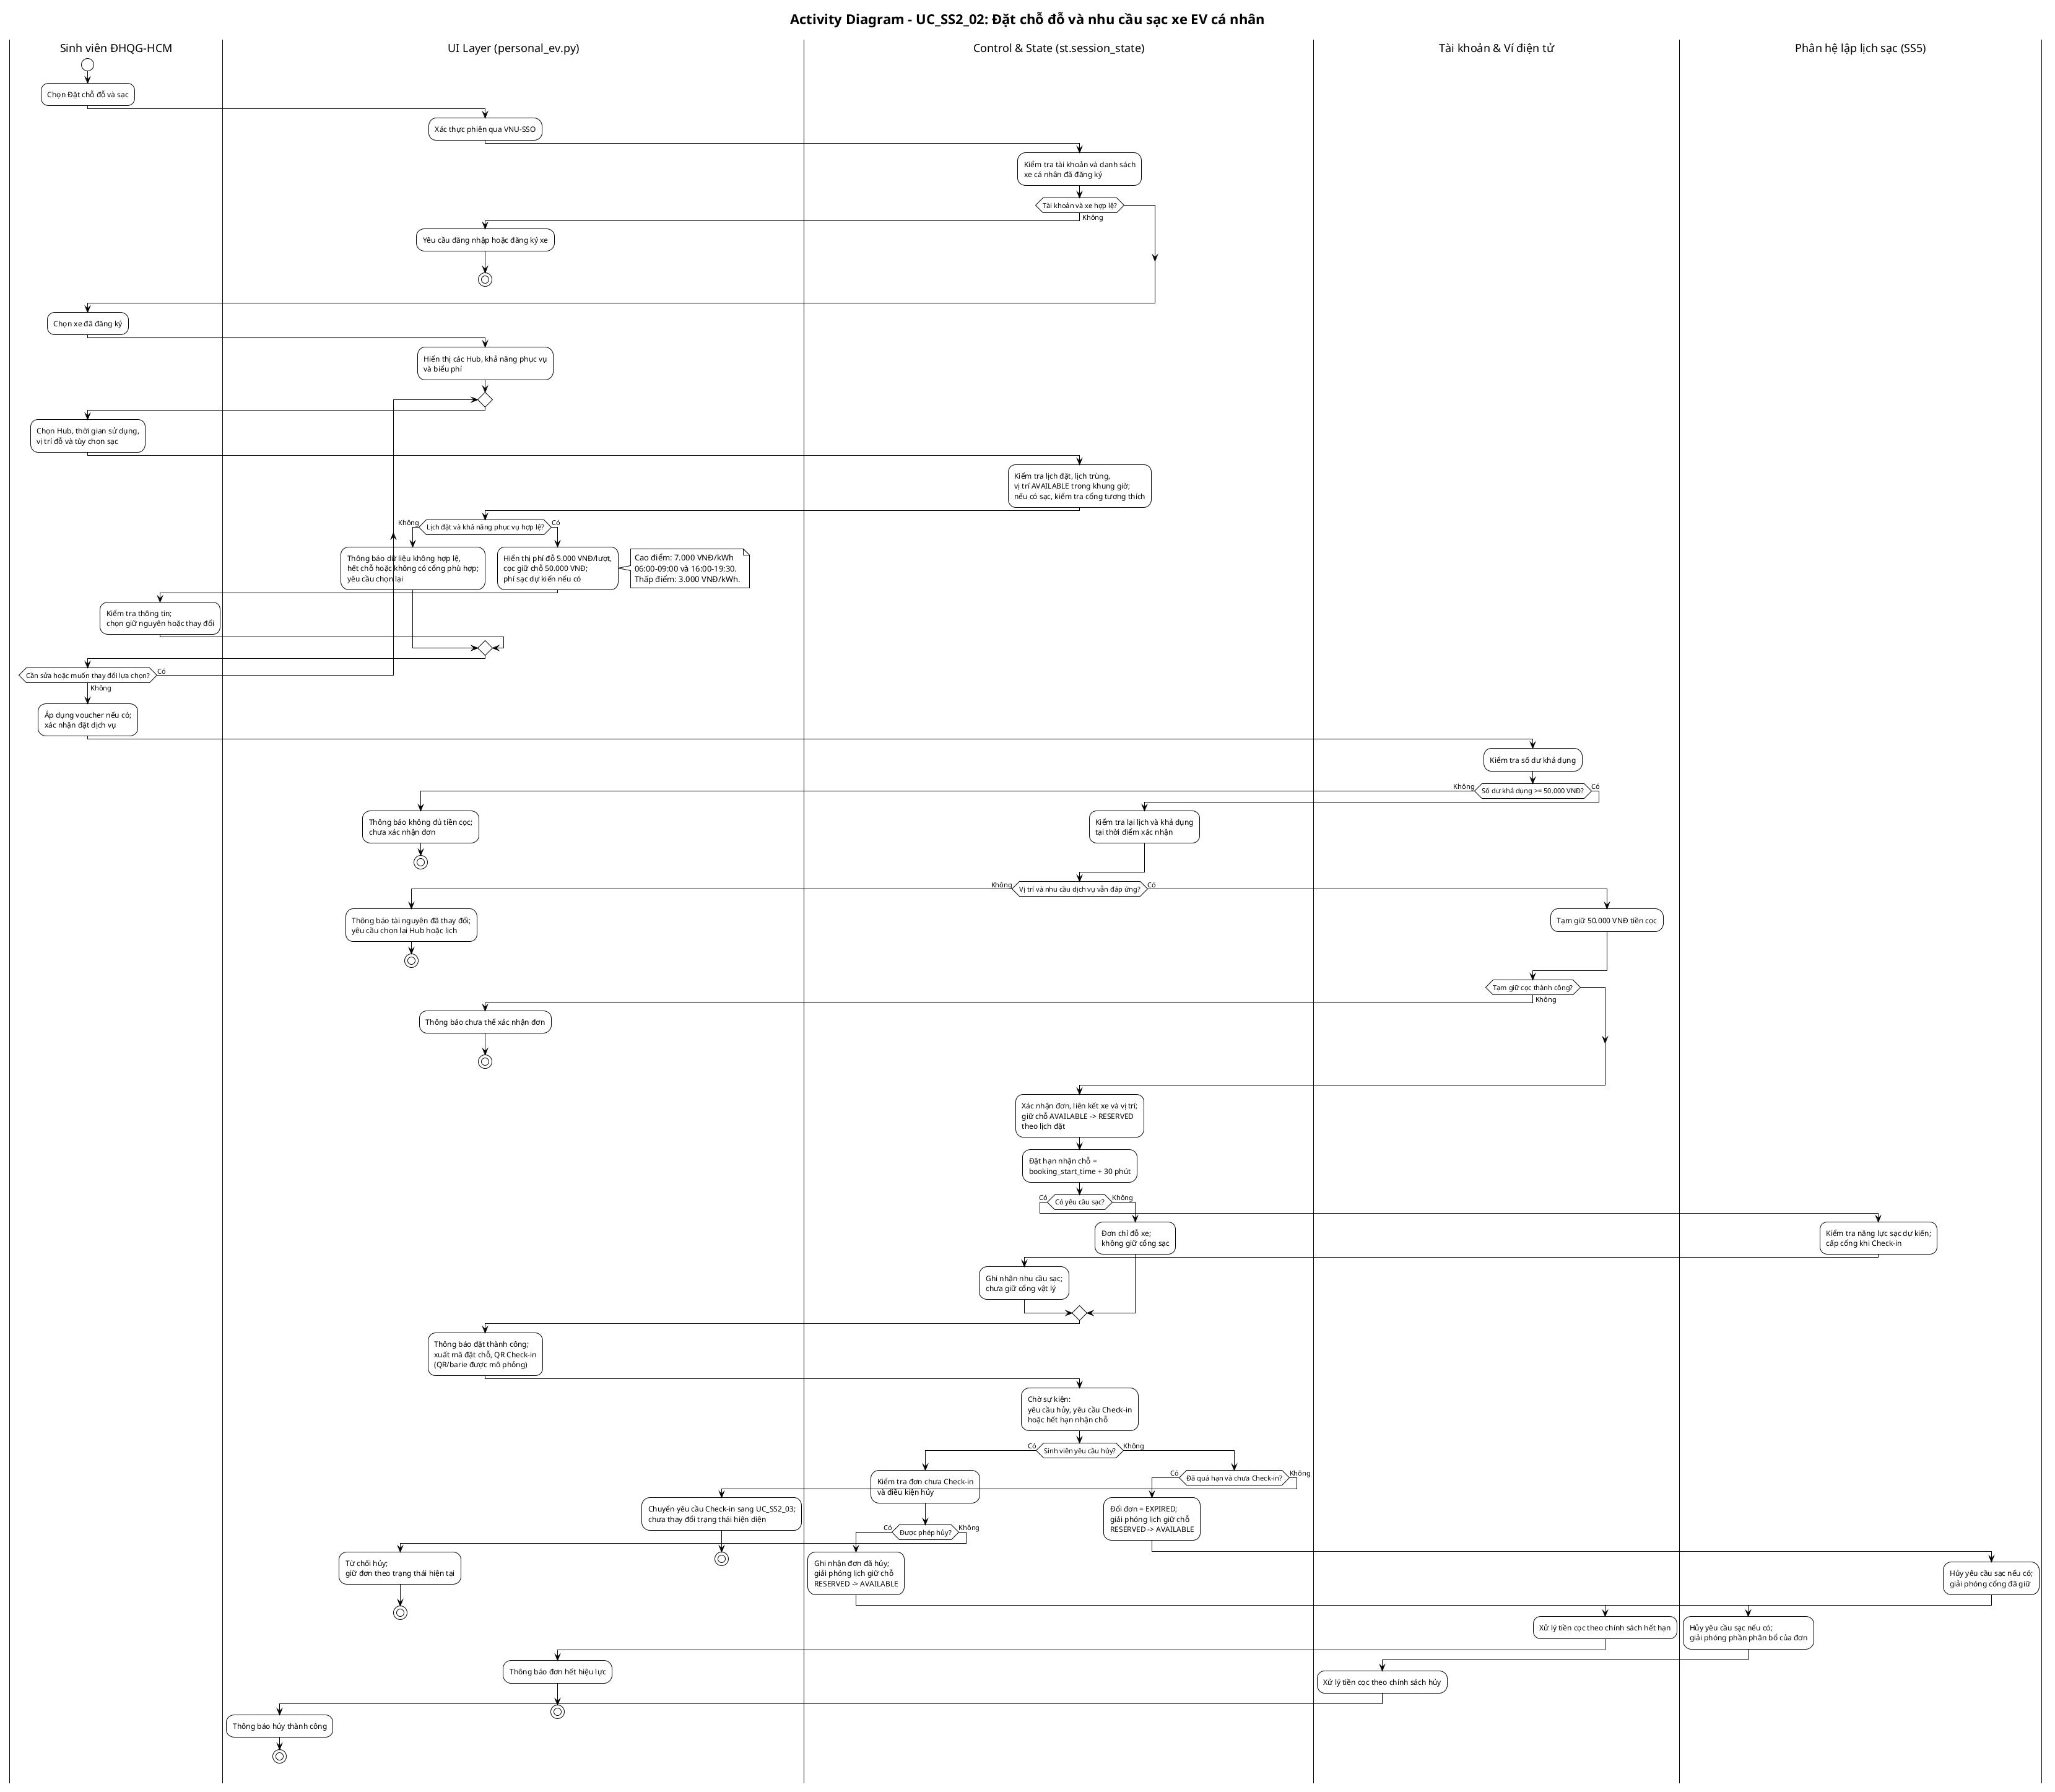
\includegraphics[width=0.92\textwidth]{Use-case detail-scenario/SS2/Activity diagrams/UC_SS2_02_NguyenAnhTai_activity.png}
    \caption{Sơ đồ Hoạt động Phân làn -- UC\_SS2\_02}
    \label{fig:act-ss2-02}
\end{figure}

\subsubsection{UC\_SS2\_03: Check-in xe EV cá nhân tại Hub}
\begin{figure}[H]
    \centering
    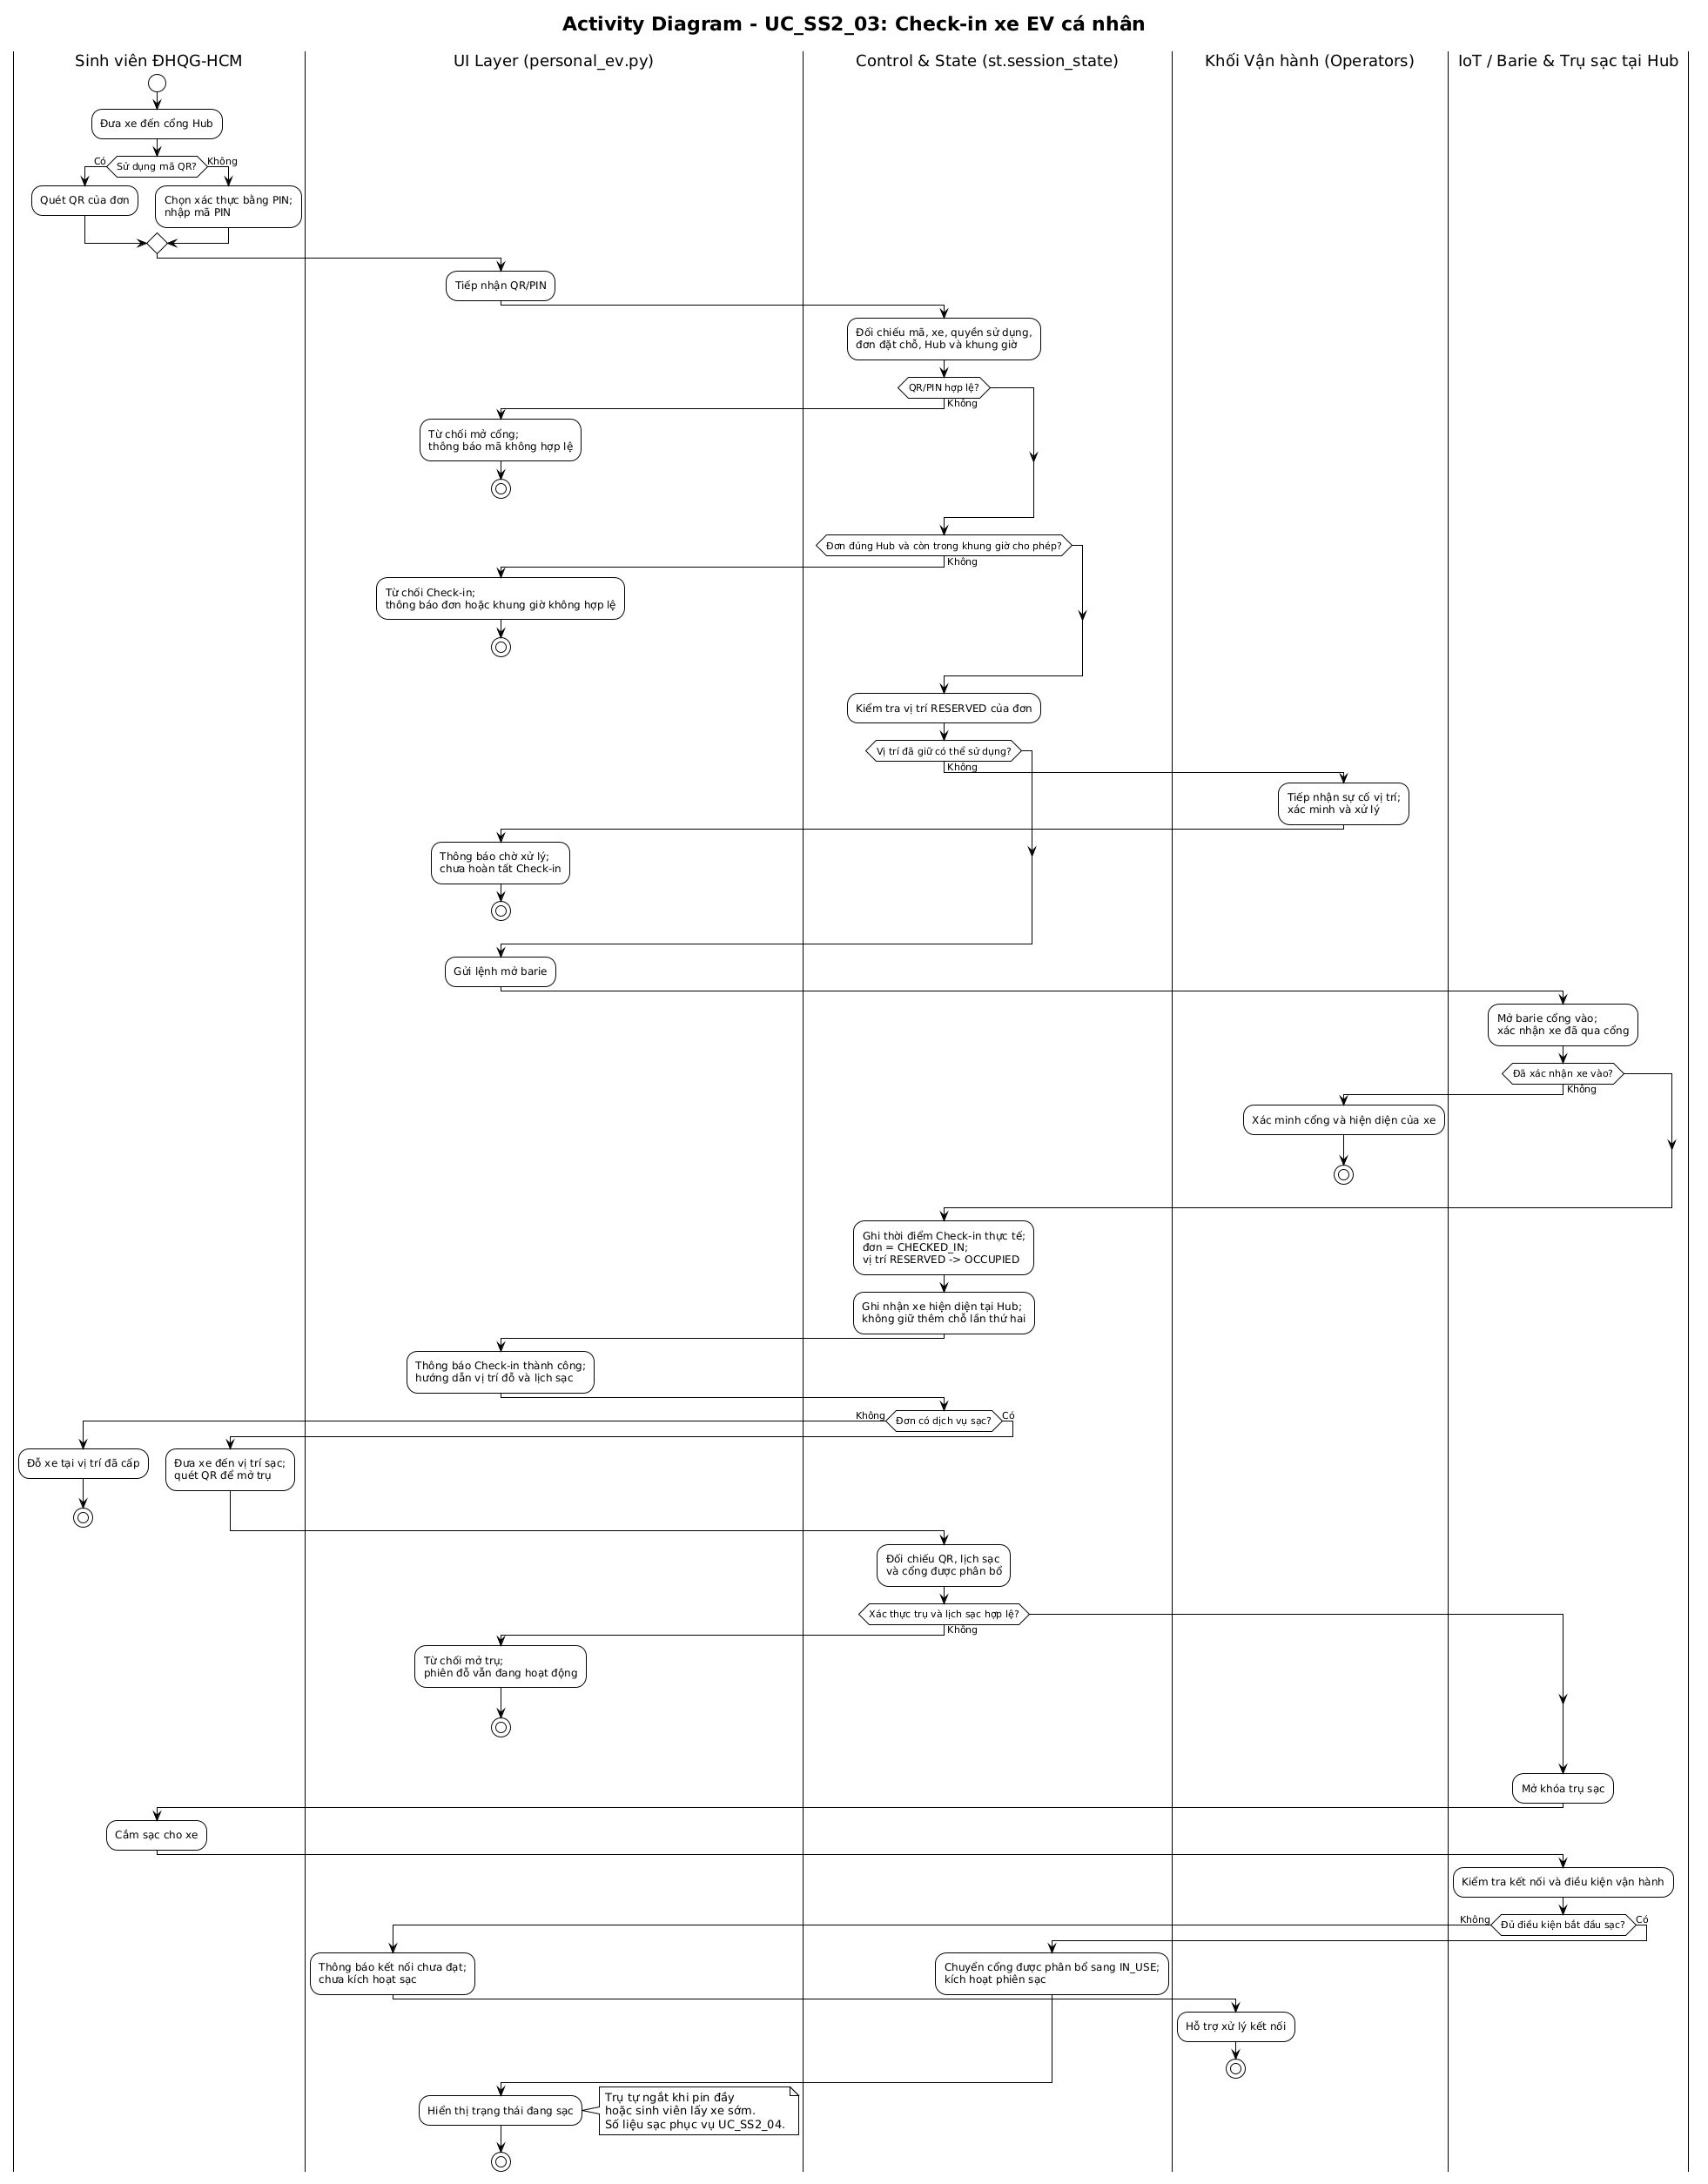
\includegraphics[width=0.92\textwidth]{Use-case detail-scenario/SS2/Activity diagrams/UC_SS2_03_NguyenAnhTai_activity.png}
    \caption{Sơ đồ Hoạt động Phân làn -- UC\_SS2\_03}
    \label{fig:act-ss2-03}
\end{figure}

\subsubsection{UC\_SS2\_04: Check-out và thanh toán dịch vụ xe cá nhân}
\begin{figure}[H]
    \centering
    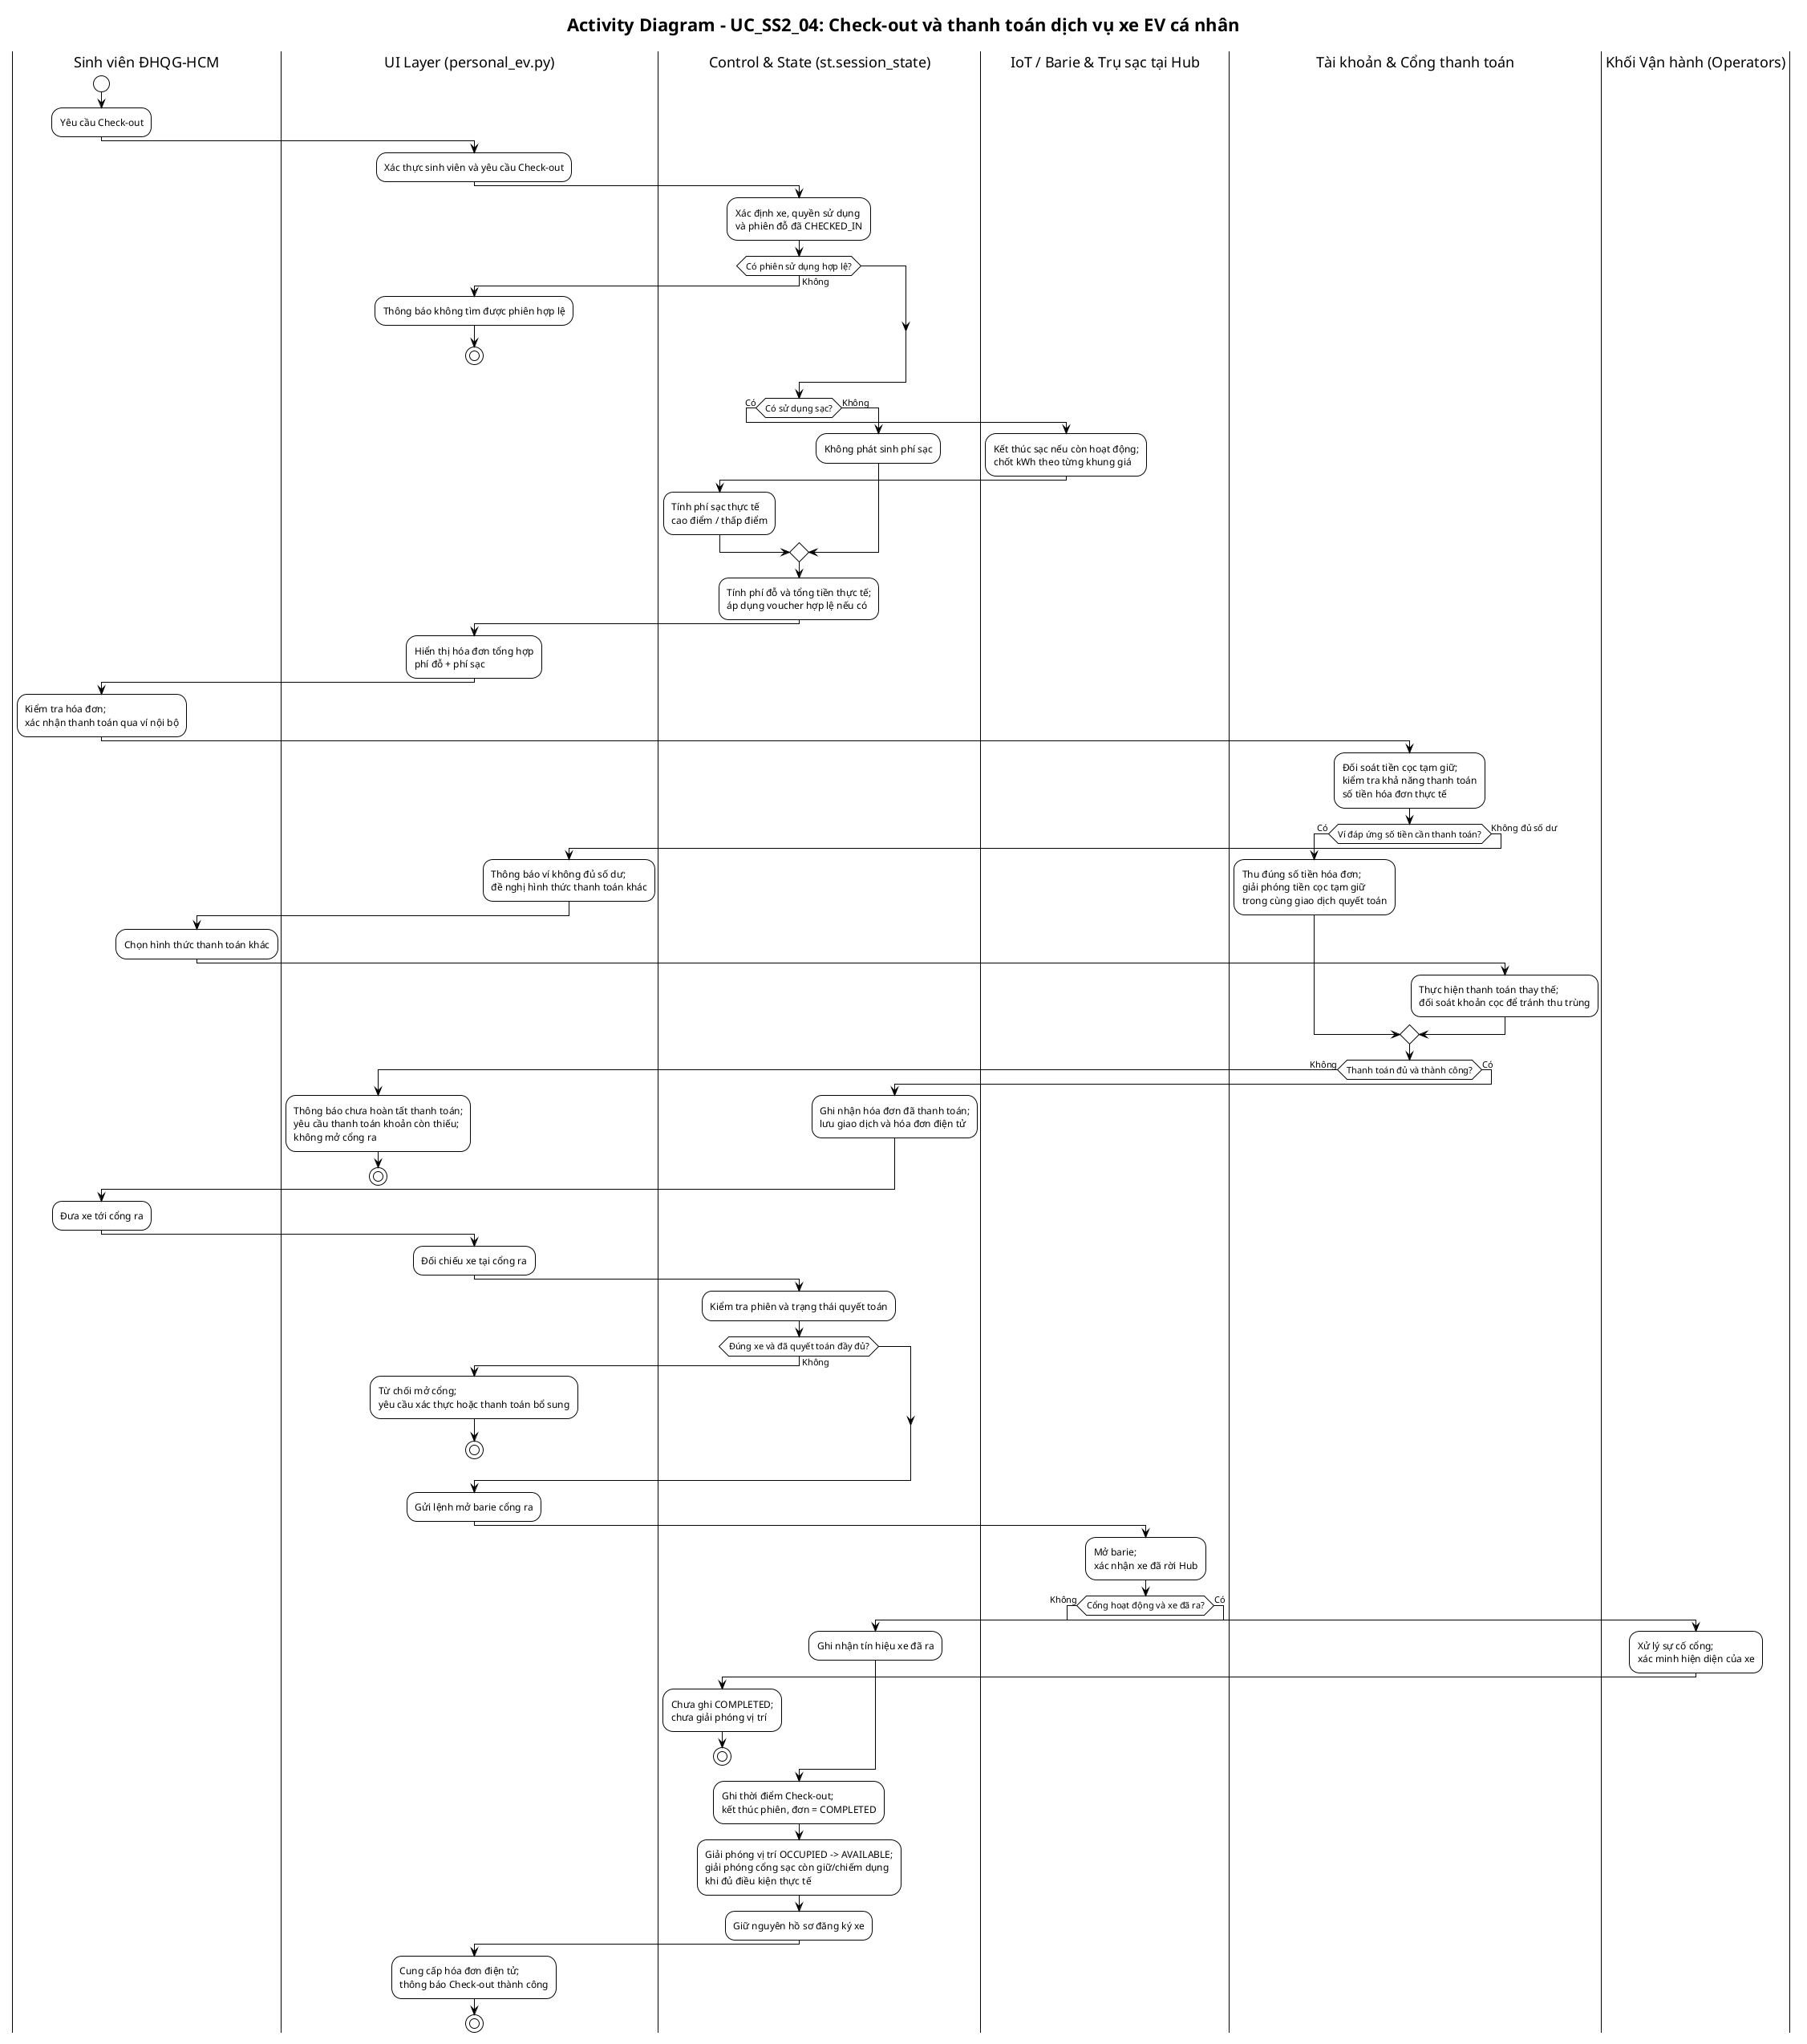
\includegraphics[width=0.92\textwidth]{Use-case detail-scenario/SS2/Activity diagrams/UC_SS2_04_NguyenAnhTai_activity.png}
    \caption{Sơ đồ Hoạt động Phân làn -- UC\_SS2\_04}
    \label{fig:act-ss2-04}
\end{figure}

\subsection{Phân hệ SS3: Giám sát Mạng lưới Hub (Phạm Tiến Đạt)}
\subsubsection{UC\_SS3\_01: Giám sát trạng thái Hub theo thời gian thực}
\begin{figure}[H]
    \centering
    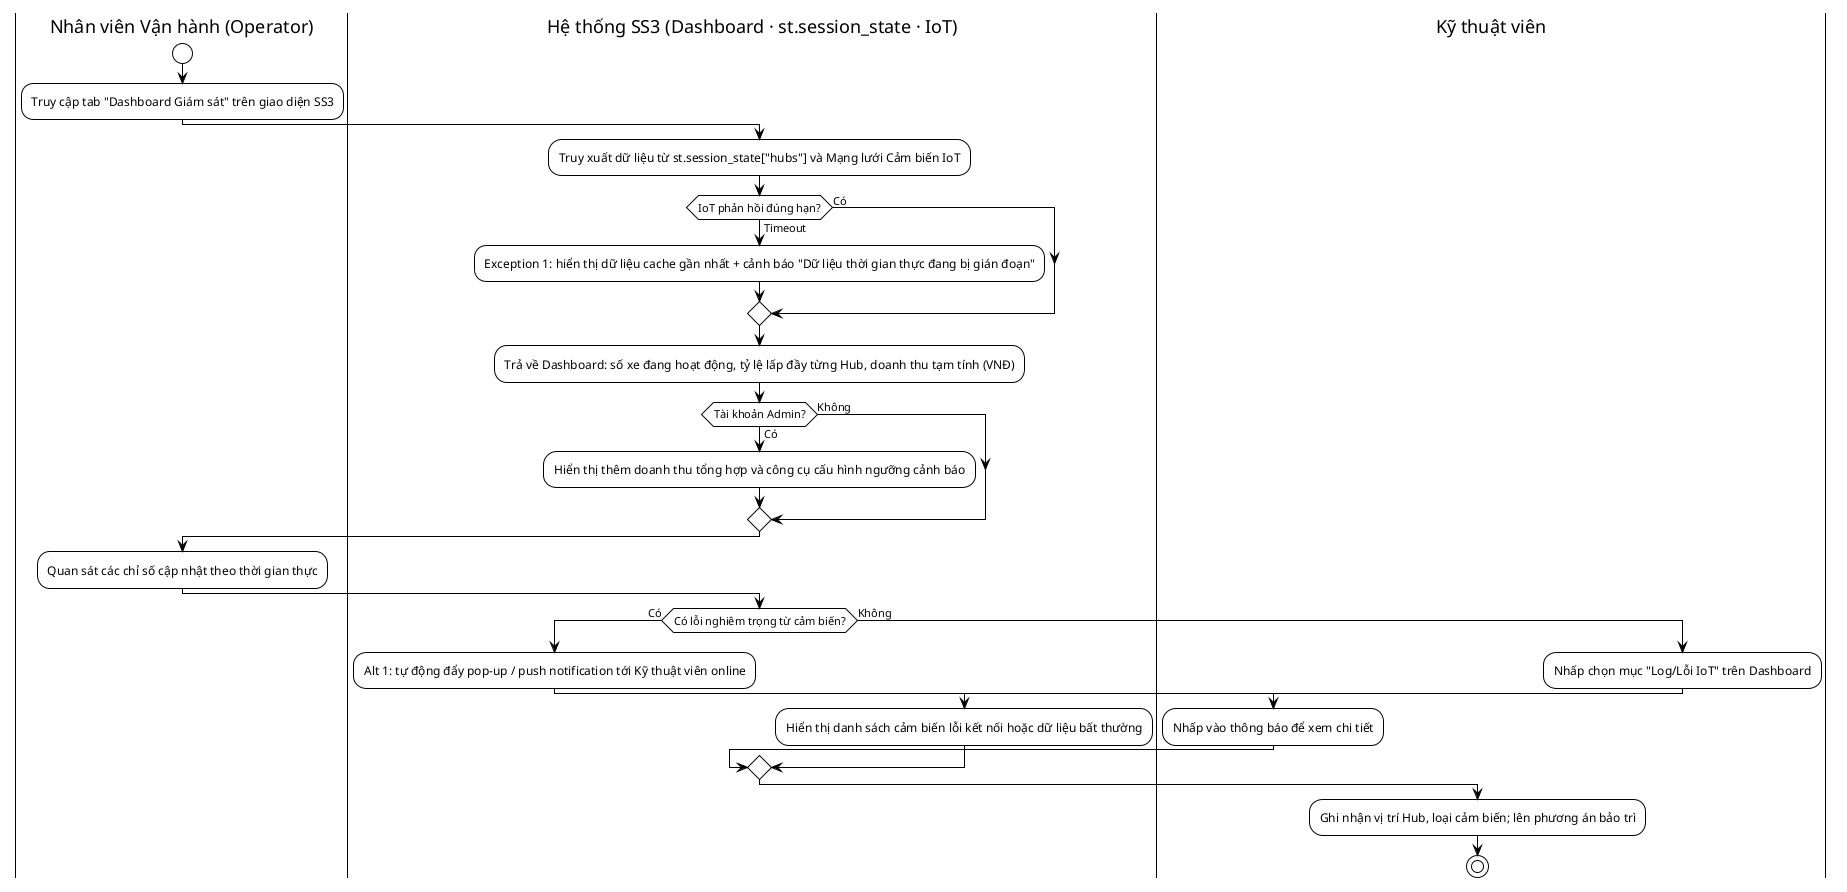
\includegraphics[width=0.92\textwidth]{Use-case detail-scenario/SS3/Activity diagrams/UC_SS3_01_PhamTienDat_activity.png}
    \caption{Sơ đồ Hoạt động Phân làn -- UC\_SS3\_01}
    \label{fig:act-ss3-01}
\end{figure}

\subsubsection{UC\_SS3\_02: Cảnh báo quá tải \& Đề xuất điều phối}
\begin{figure}[H]
    \centering
    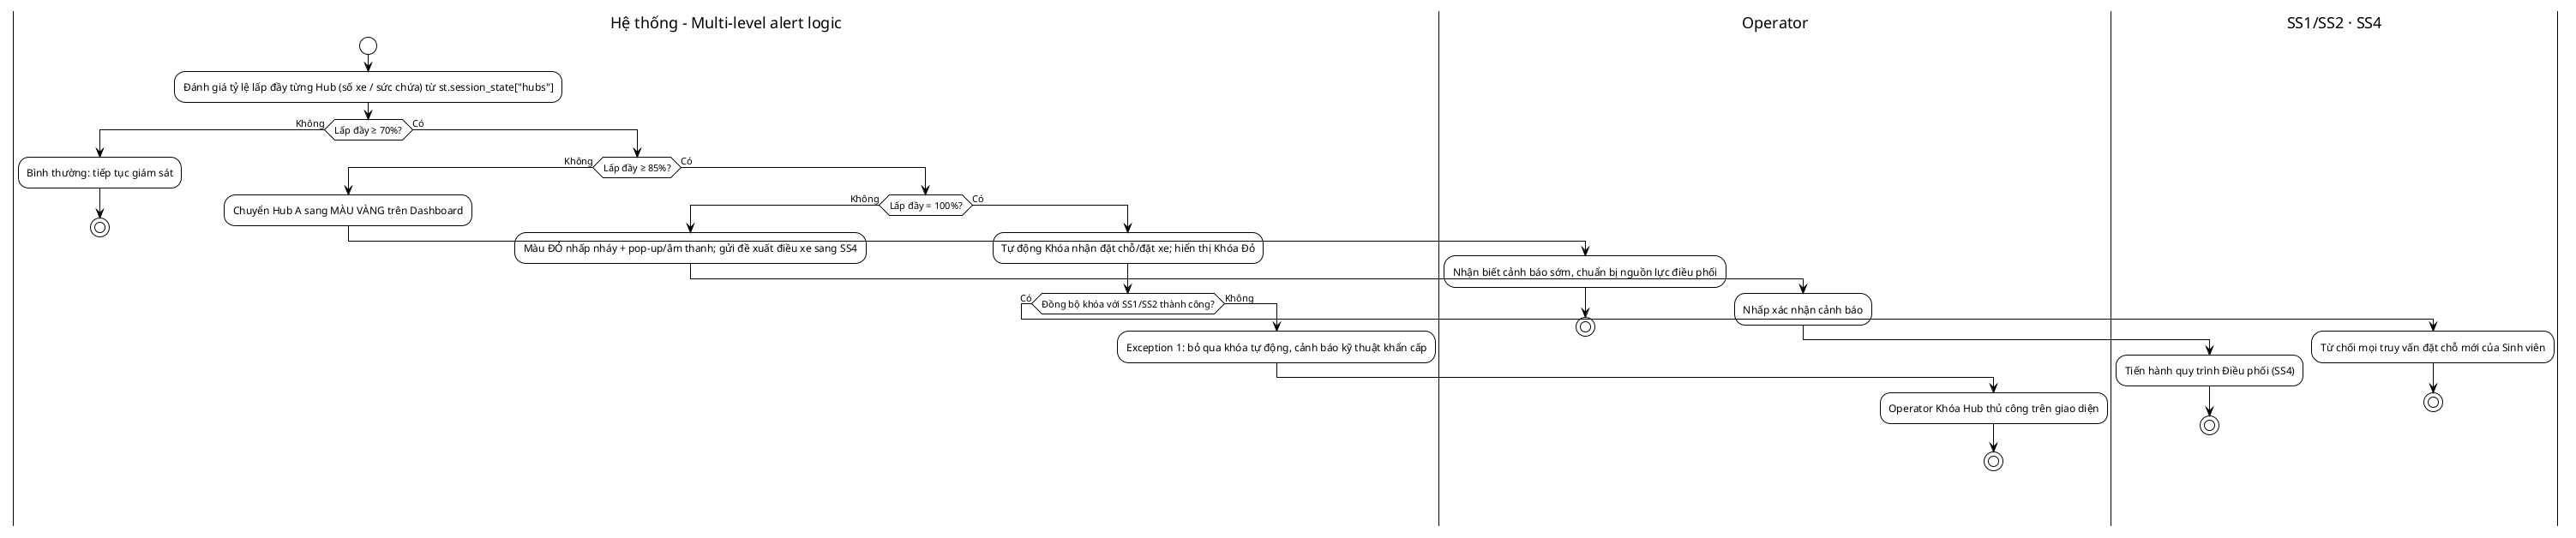
\includegraphics[width=0.92\textwidth]{Use-case detail-scenario/SS3/Activity diagrams/UC_SS3_02_PhamTienDat_activity.png}
    \caption{Sơ đồ Hoạt động Phân làn -- UC\_SS3\_02}
    \label{fig:act-ss3-02}
\end{figure}

\subsection{Phân hệ SS4: Điều phối \& Xử lý Sự cố (Đặng Hoàng Quý Nhân)}
\subsubsection{UC\_SS4\_01: Lập lệnh điều phối phương tiện giữa các Hub}
\begin{figure}[H]
    \centering
    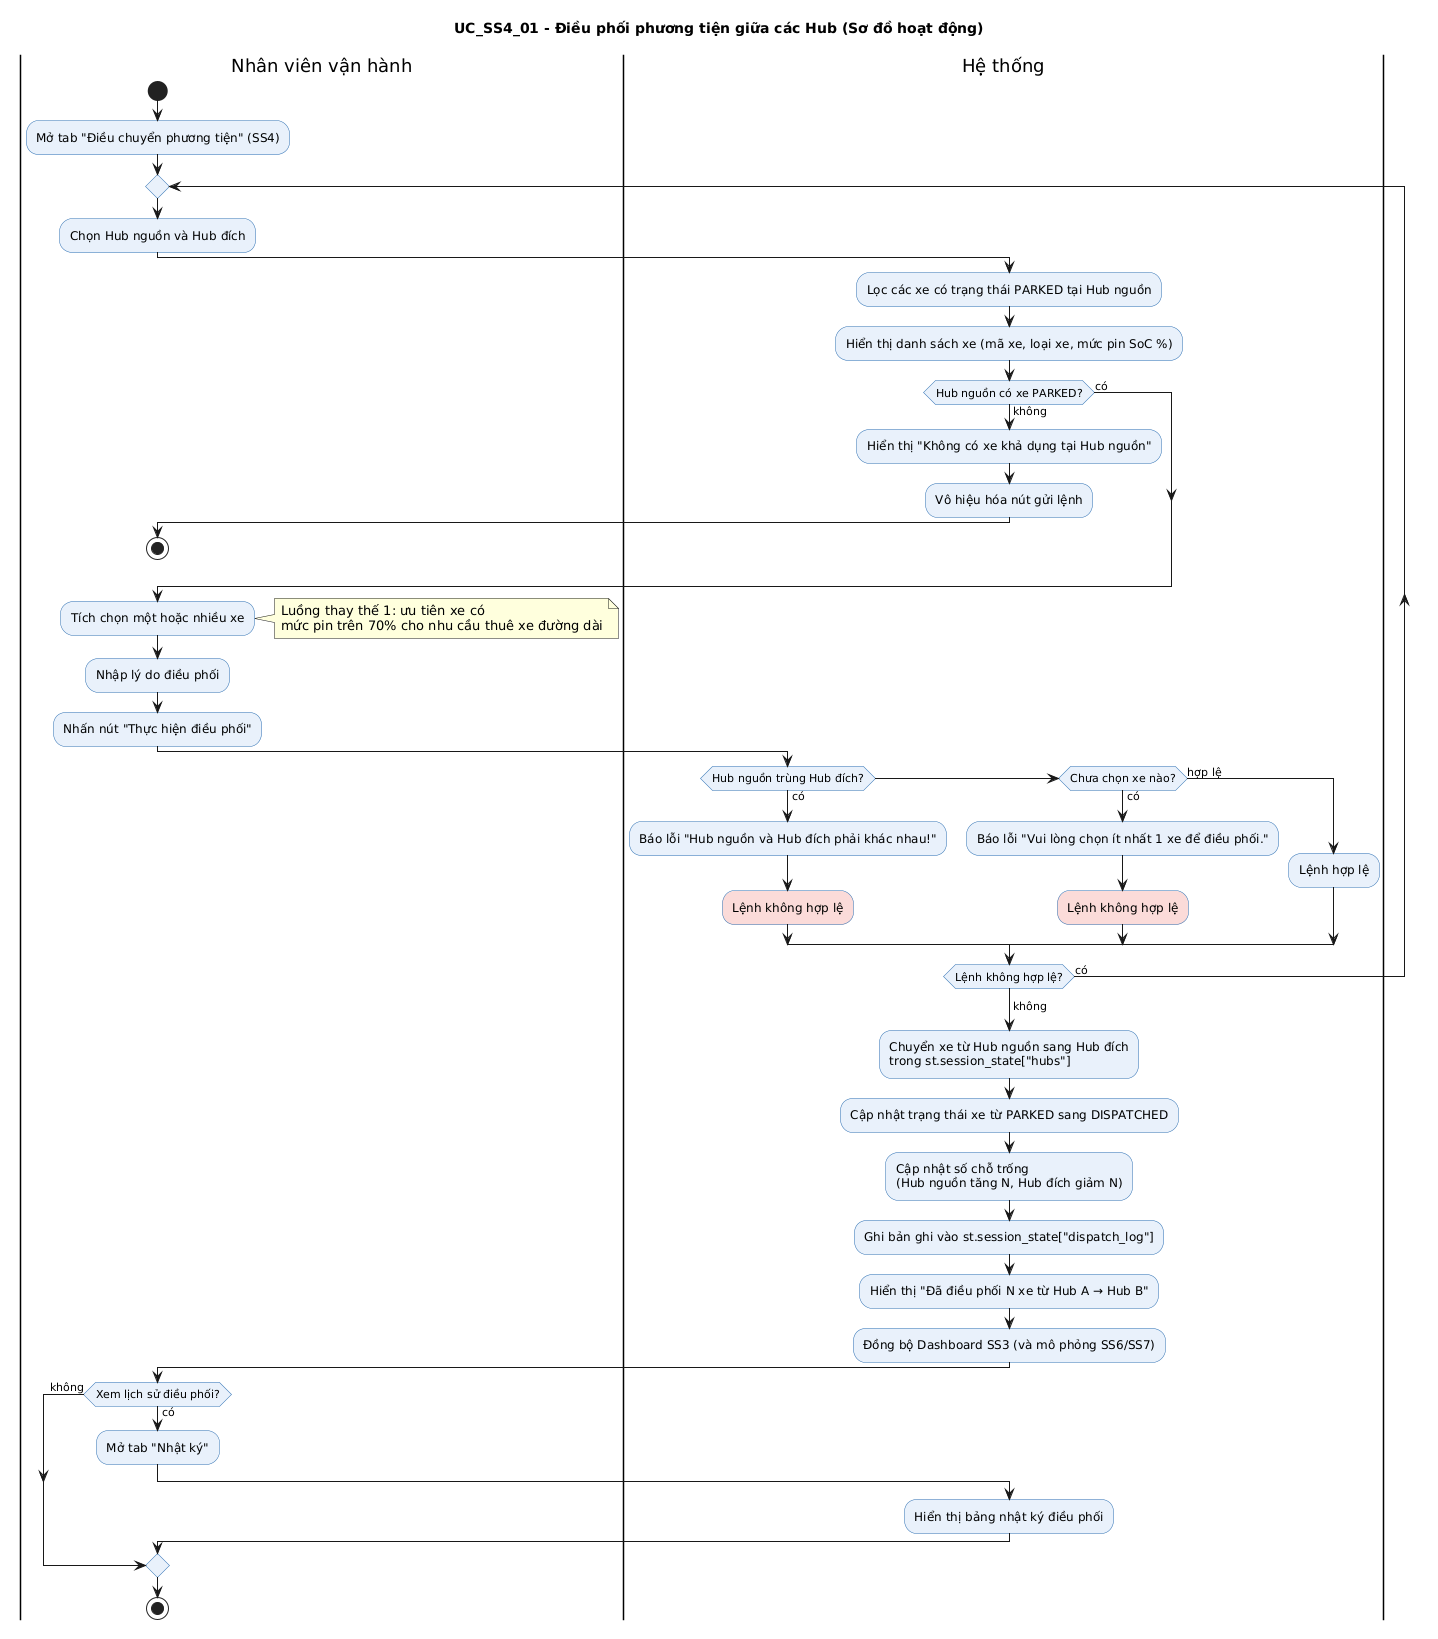
\includegraphics[width=0.92\textwidth]{Use-case detail-scenario/SS4/Activity diagrams/UC_SS4_01_activity.png}
    \caption{Sơ đồ Hoạt động Phân làn -- UC\_SS4\_01}
    \label{fig:act-ss4-01}
\end{figure}

\subsubsection{UC\_SS4\_02: Báo cáo \& Xử lý sự cố kỹ thuật phương tiện}
\begin{figure}[H]
    \centering
    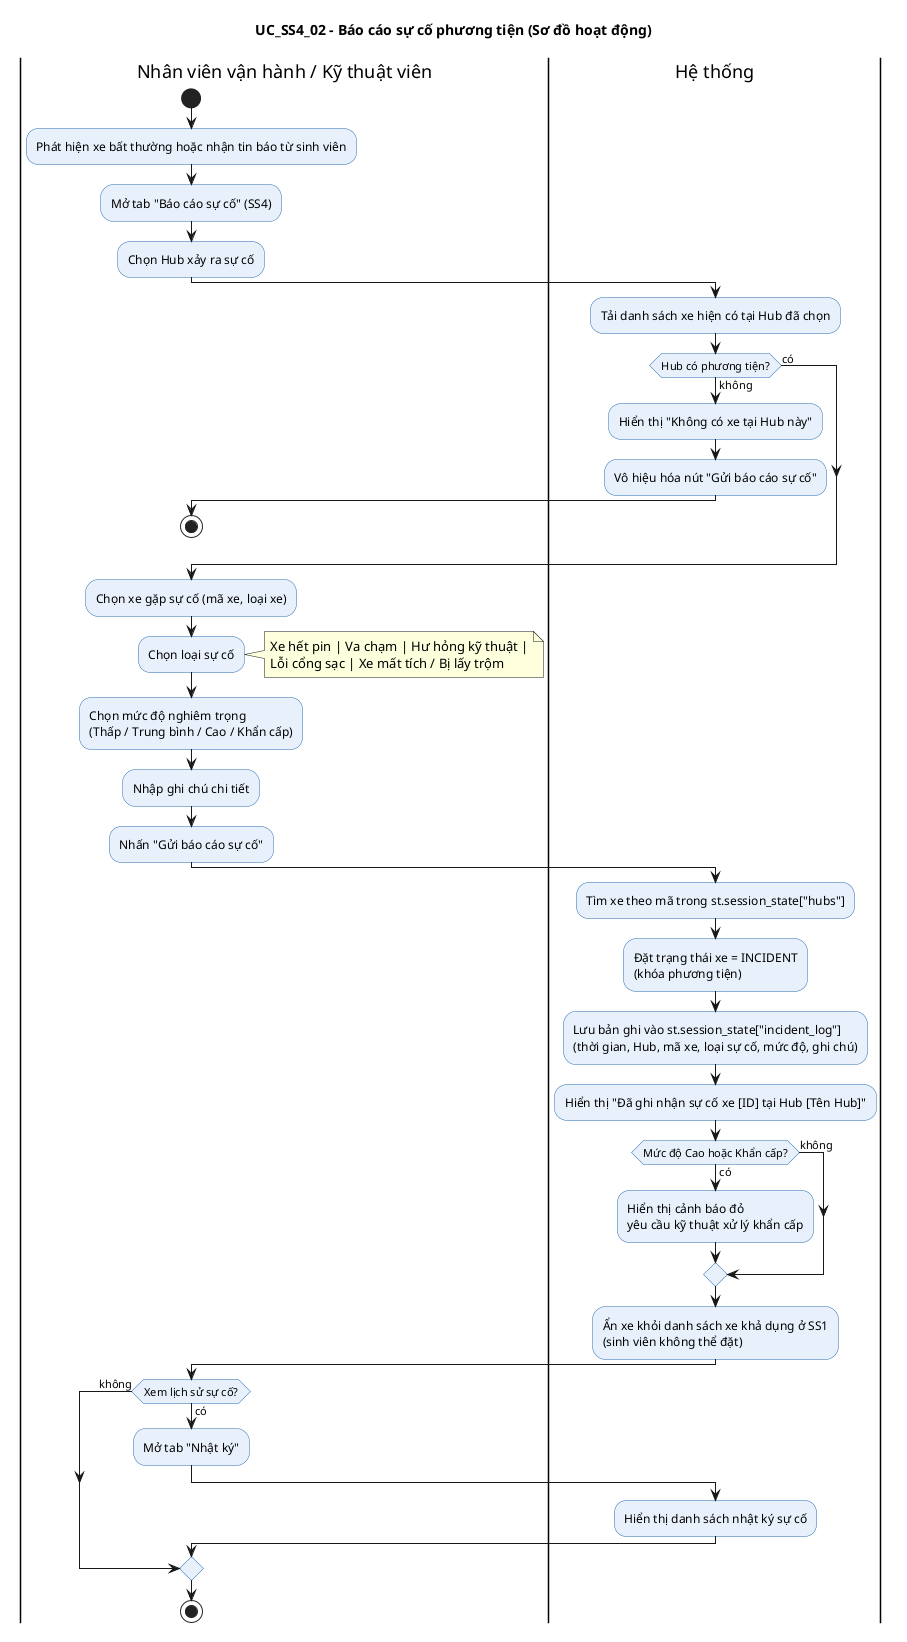
\includegraphics[width=0.92\textwidth]{Use-case detail-scenario/SS4/Activity diagrams/UC_SS4_02_activity.png}
    \caption{Sơ đồ Hoạt động Phân làn -- UC\_SS4\_02}
    \label{fig:act-ss4-02}
\end{figure}

\subsection{Phân hệ SS5: Lập lịch Sạc Thông minh (Dương Đăng Khoa)}
\subsubsection{UC\_SS5\_01: Lập lịch ưu tiên sạc tự động}
\begin{figure}[H]
    \centering
    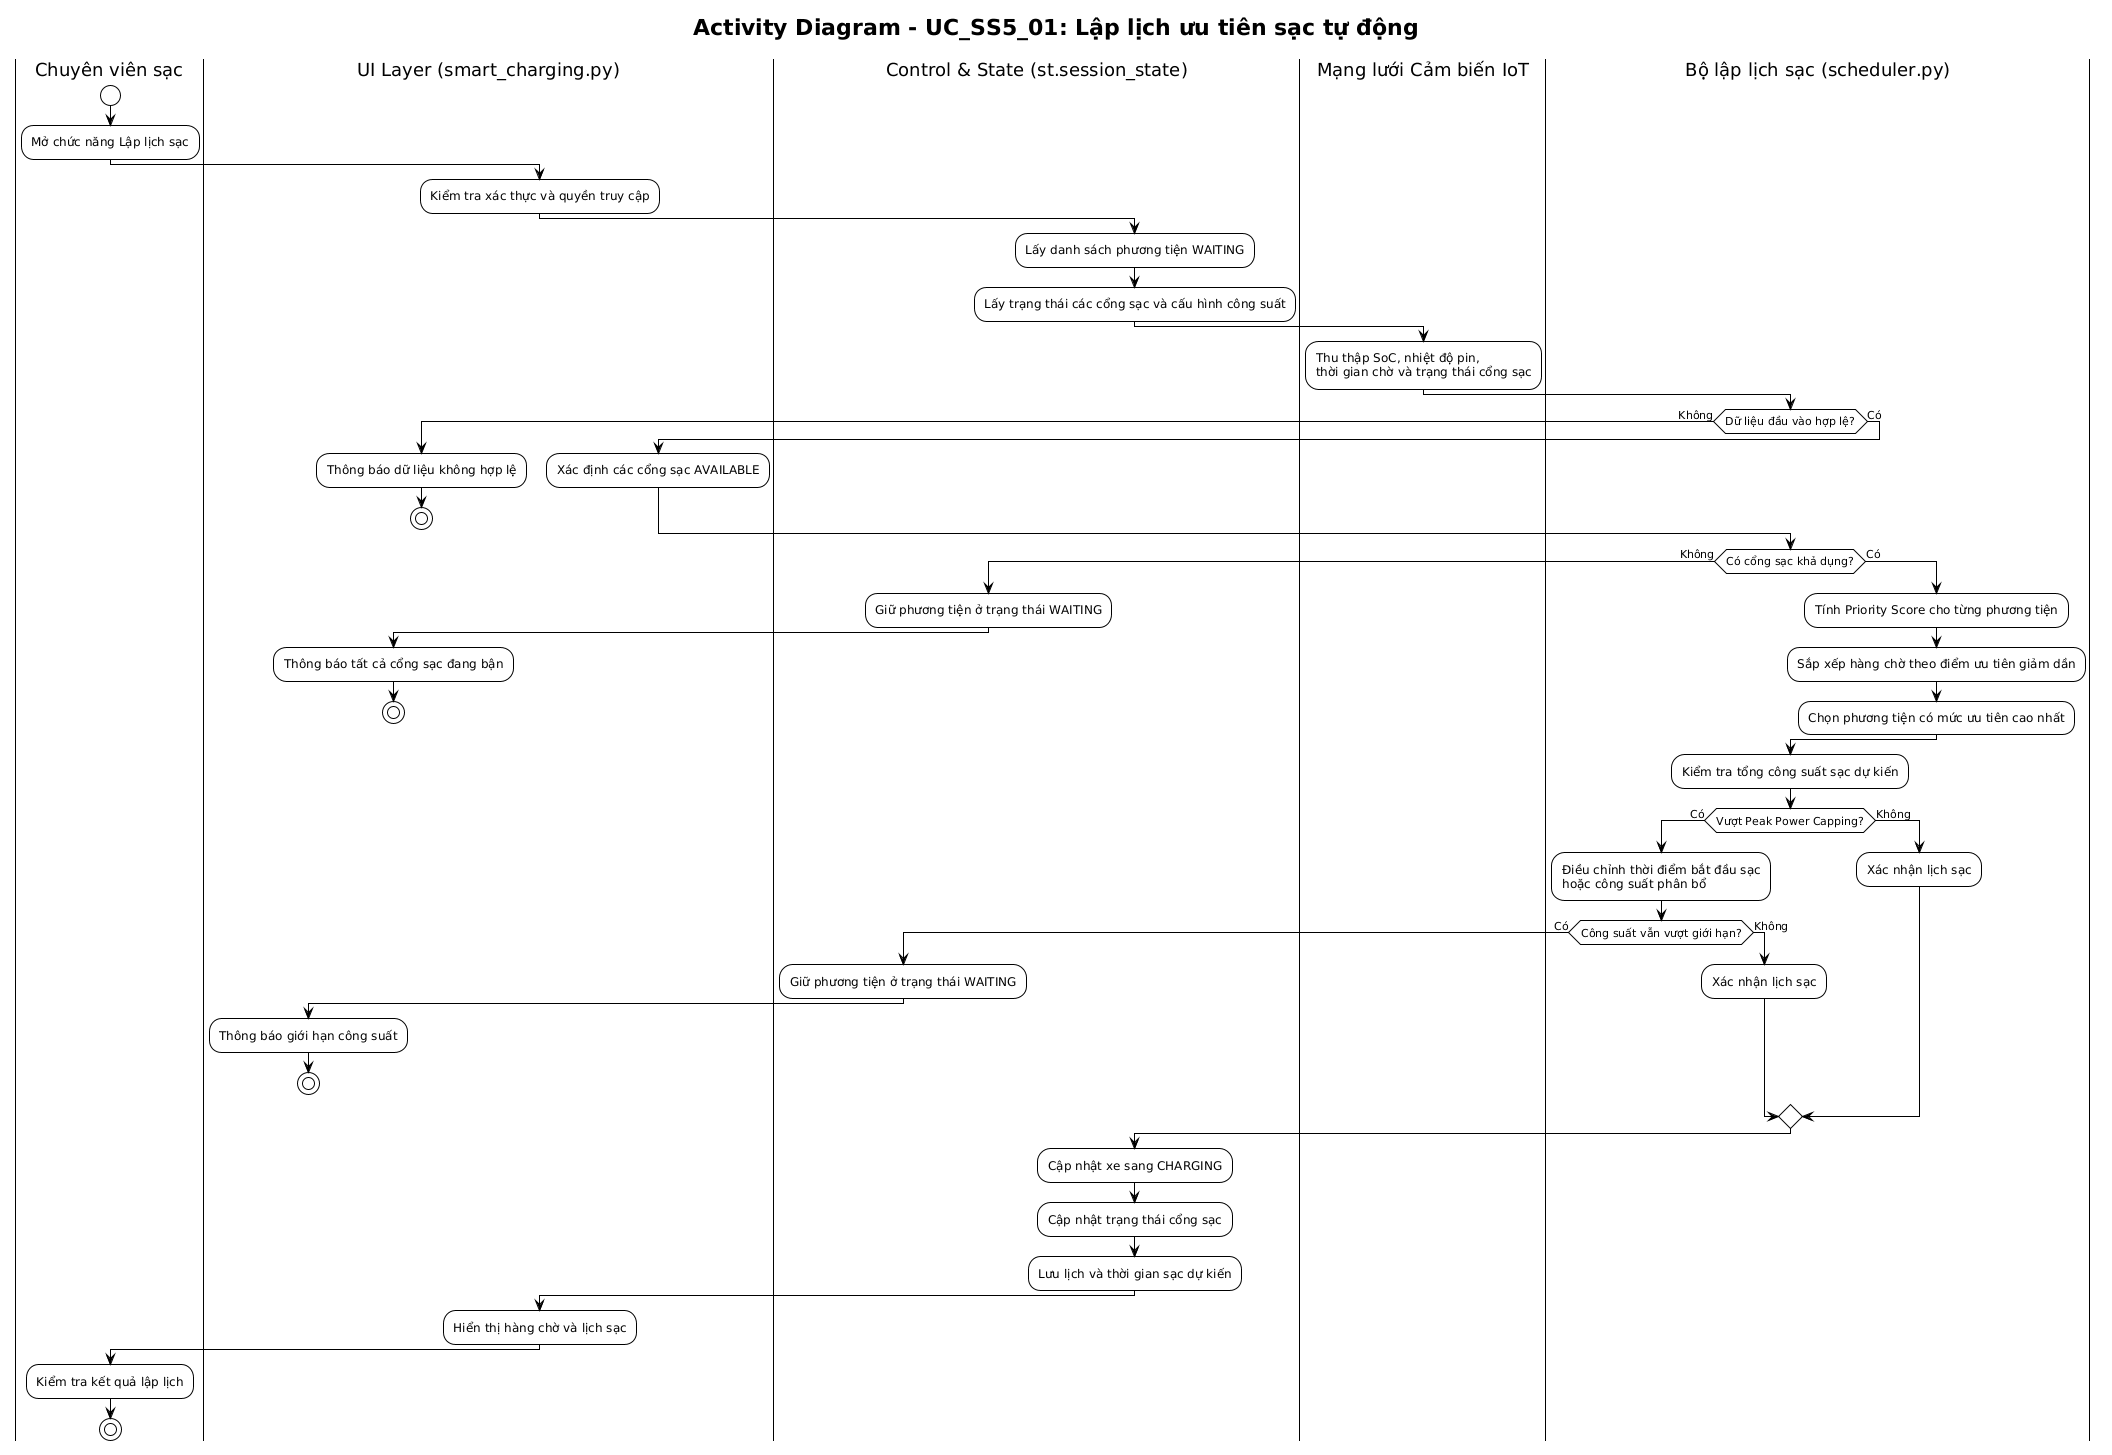
\includegraphics[width=0.92\textwidth]{Use-case detail-scenario/SS5/Activity diagrams/UC_SS5_01_DuongDangKhoa_activity.png}
    \caption{Sơ đồ Hoạt động Phân làn -- UC\_SS5\_01}
    \label{fig:act-ss5-01}
\end{figure}

\subsubsection{UC\_SS5\_02: Giám sát hàng đợi sạc \& Phí chiếm dụng}
\begin{figure}[H]
    \centering
    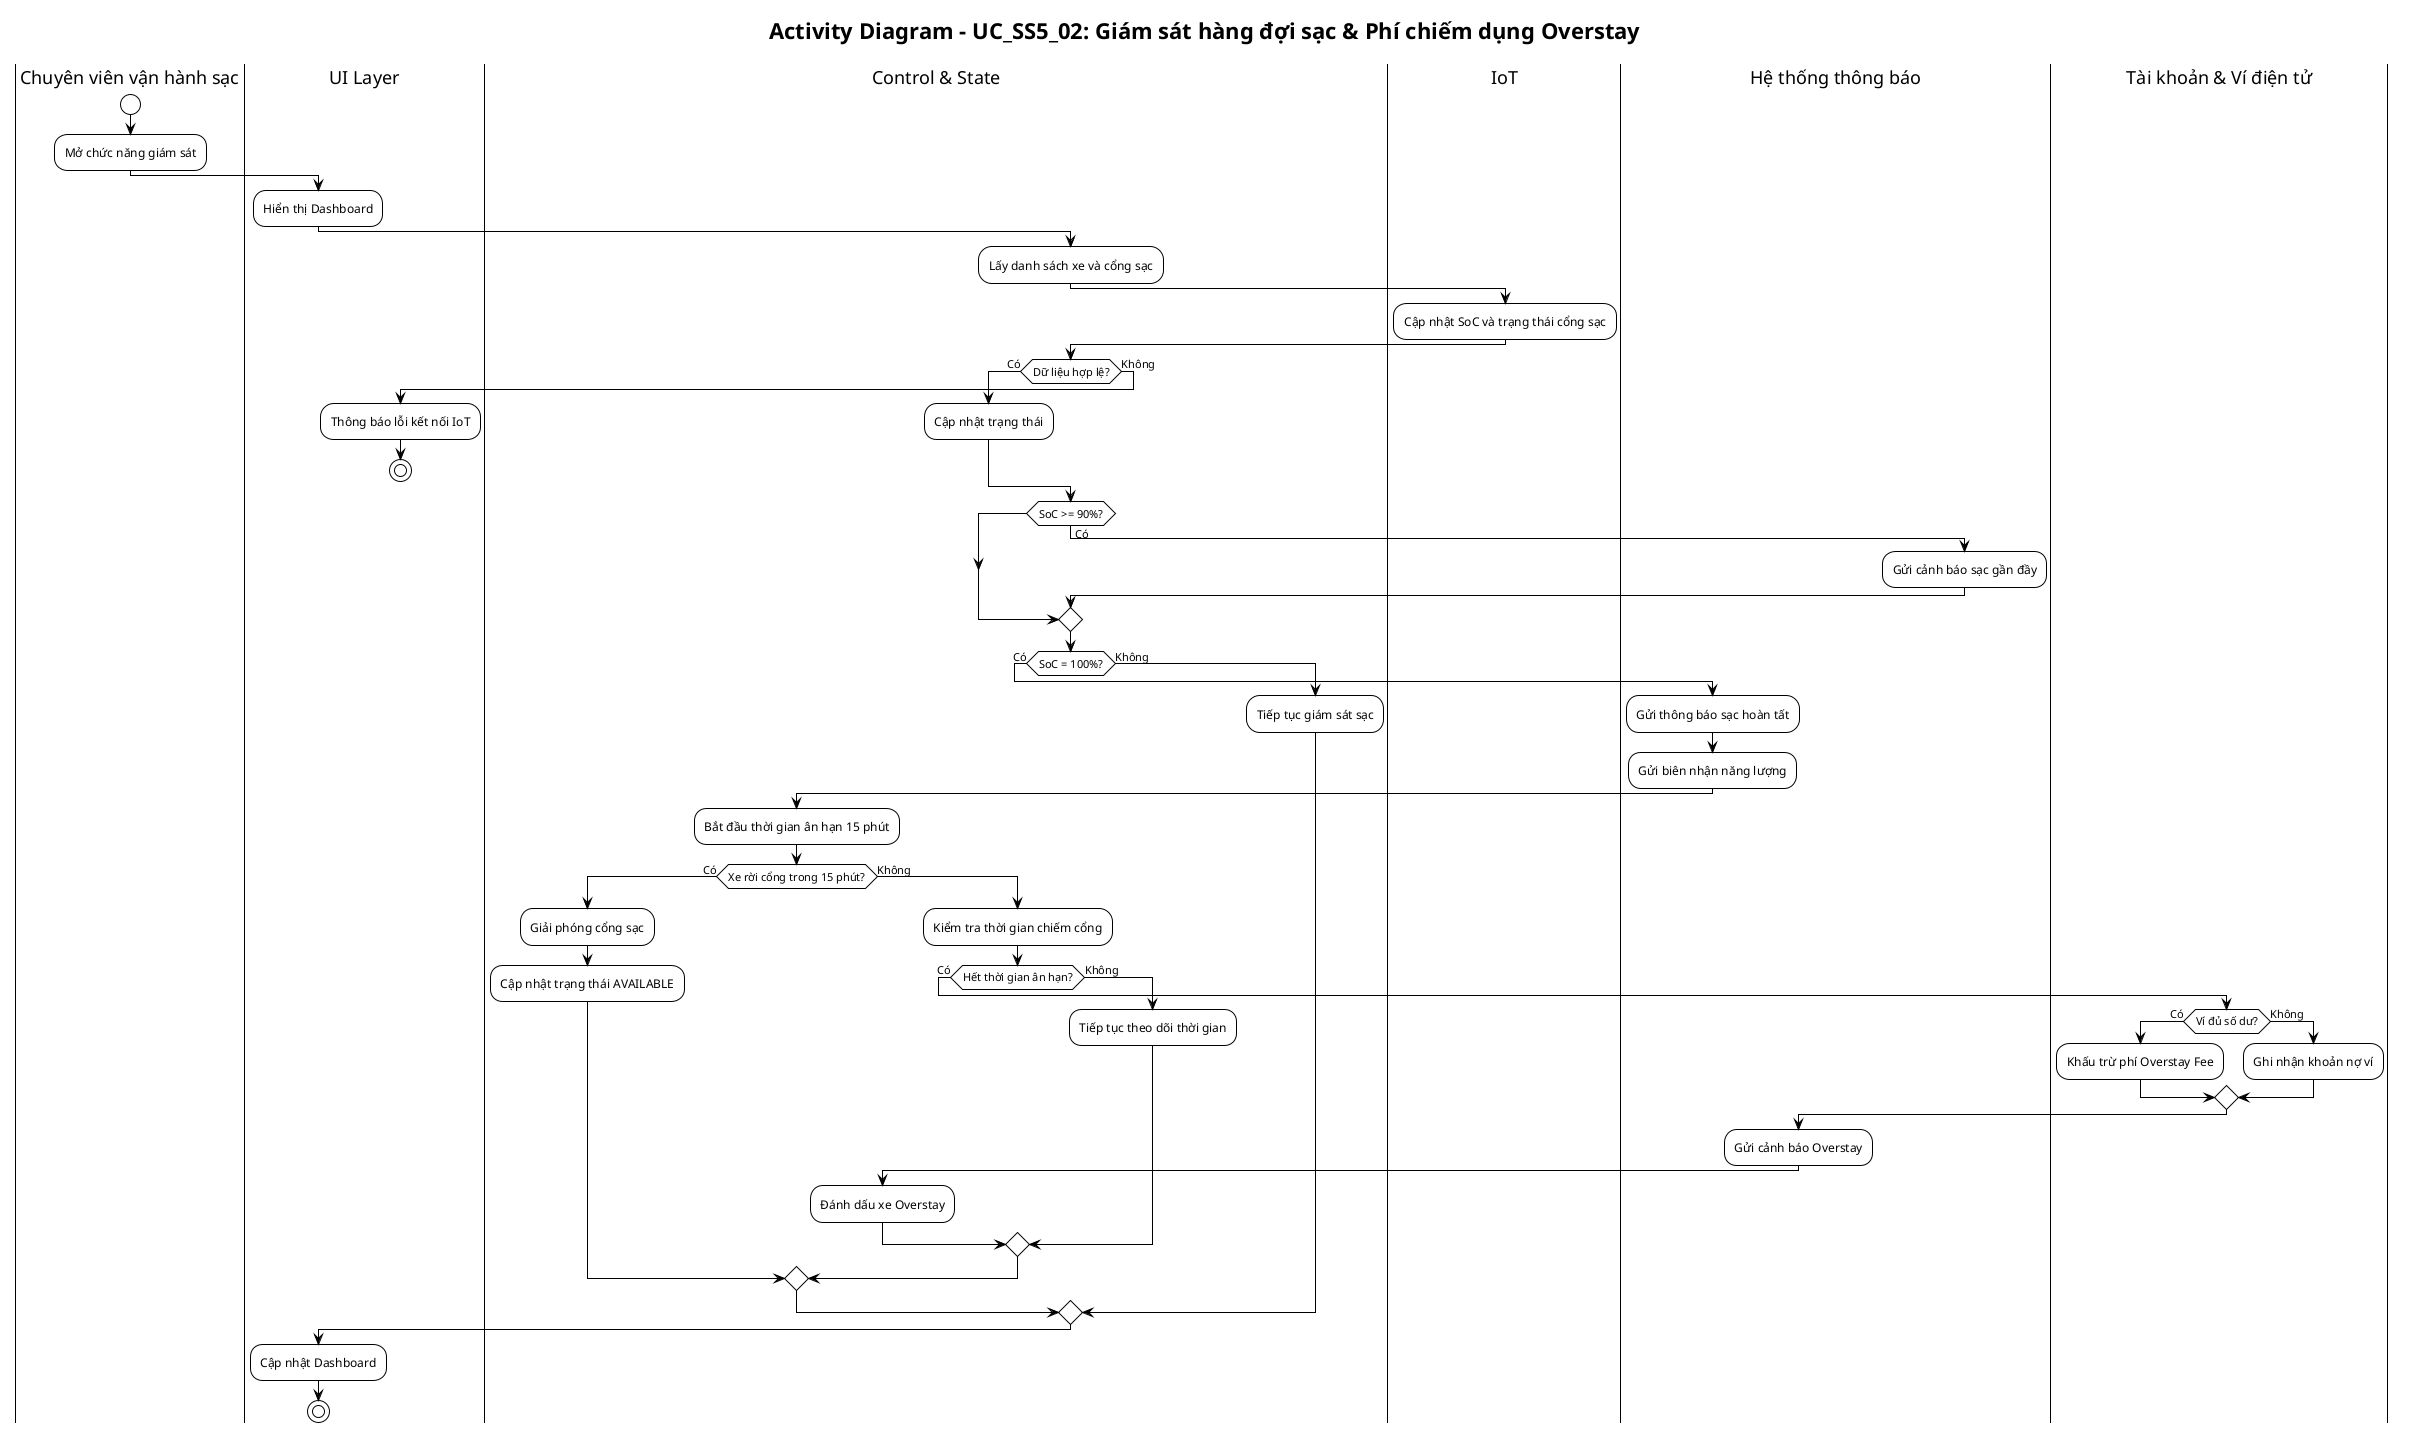
\includegraphics[width=0.92\textwidth]{Use-case detail-scenario/SS5/Activity diagrams/UC_SS5_02_DuongDangKhoa_activity.png}
    \caption{Sơ đồ Hoạt động Phân làn -- UC\_SS5\_02}
    \label{fig:act-ss5-02}
\end{figure}

\subsection{Phân hệ SS6: Mô phỏng What-if Nhu cầu (Hoàng Văn Tấn)}
\subsubsection{UC\_SS6\_01: Mô phỏng đợt tăng đột biến hành khách Metro (Metro Surge)}
\begin{figure}[H]
    \centering
    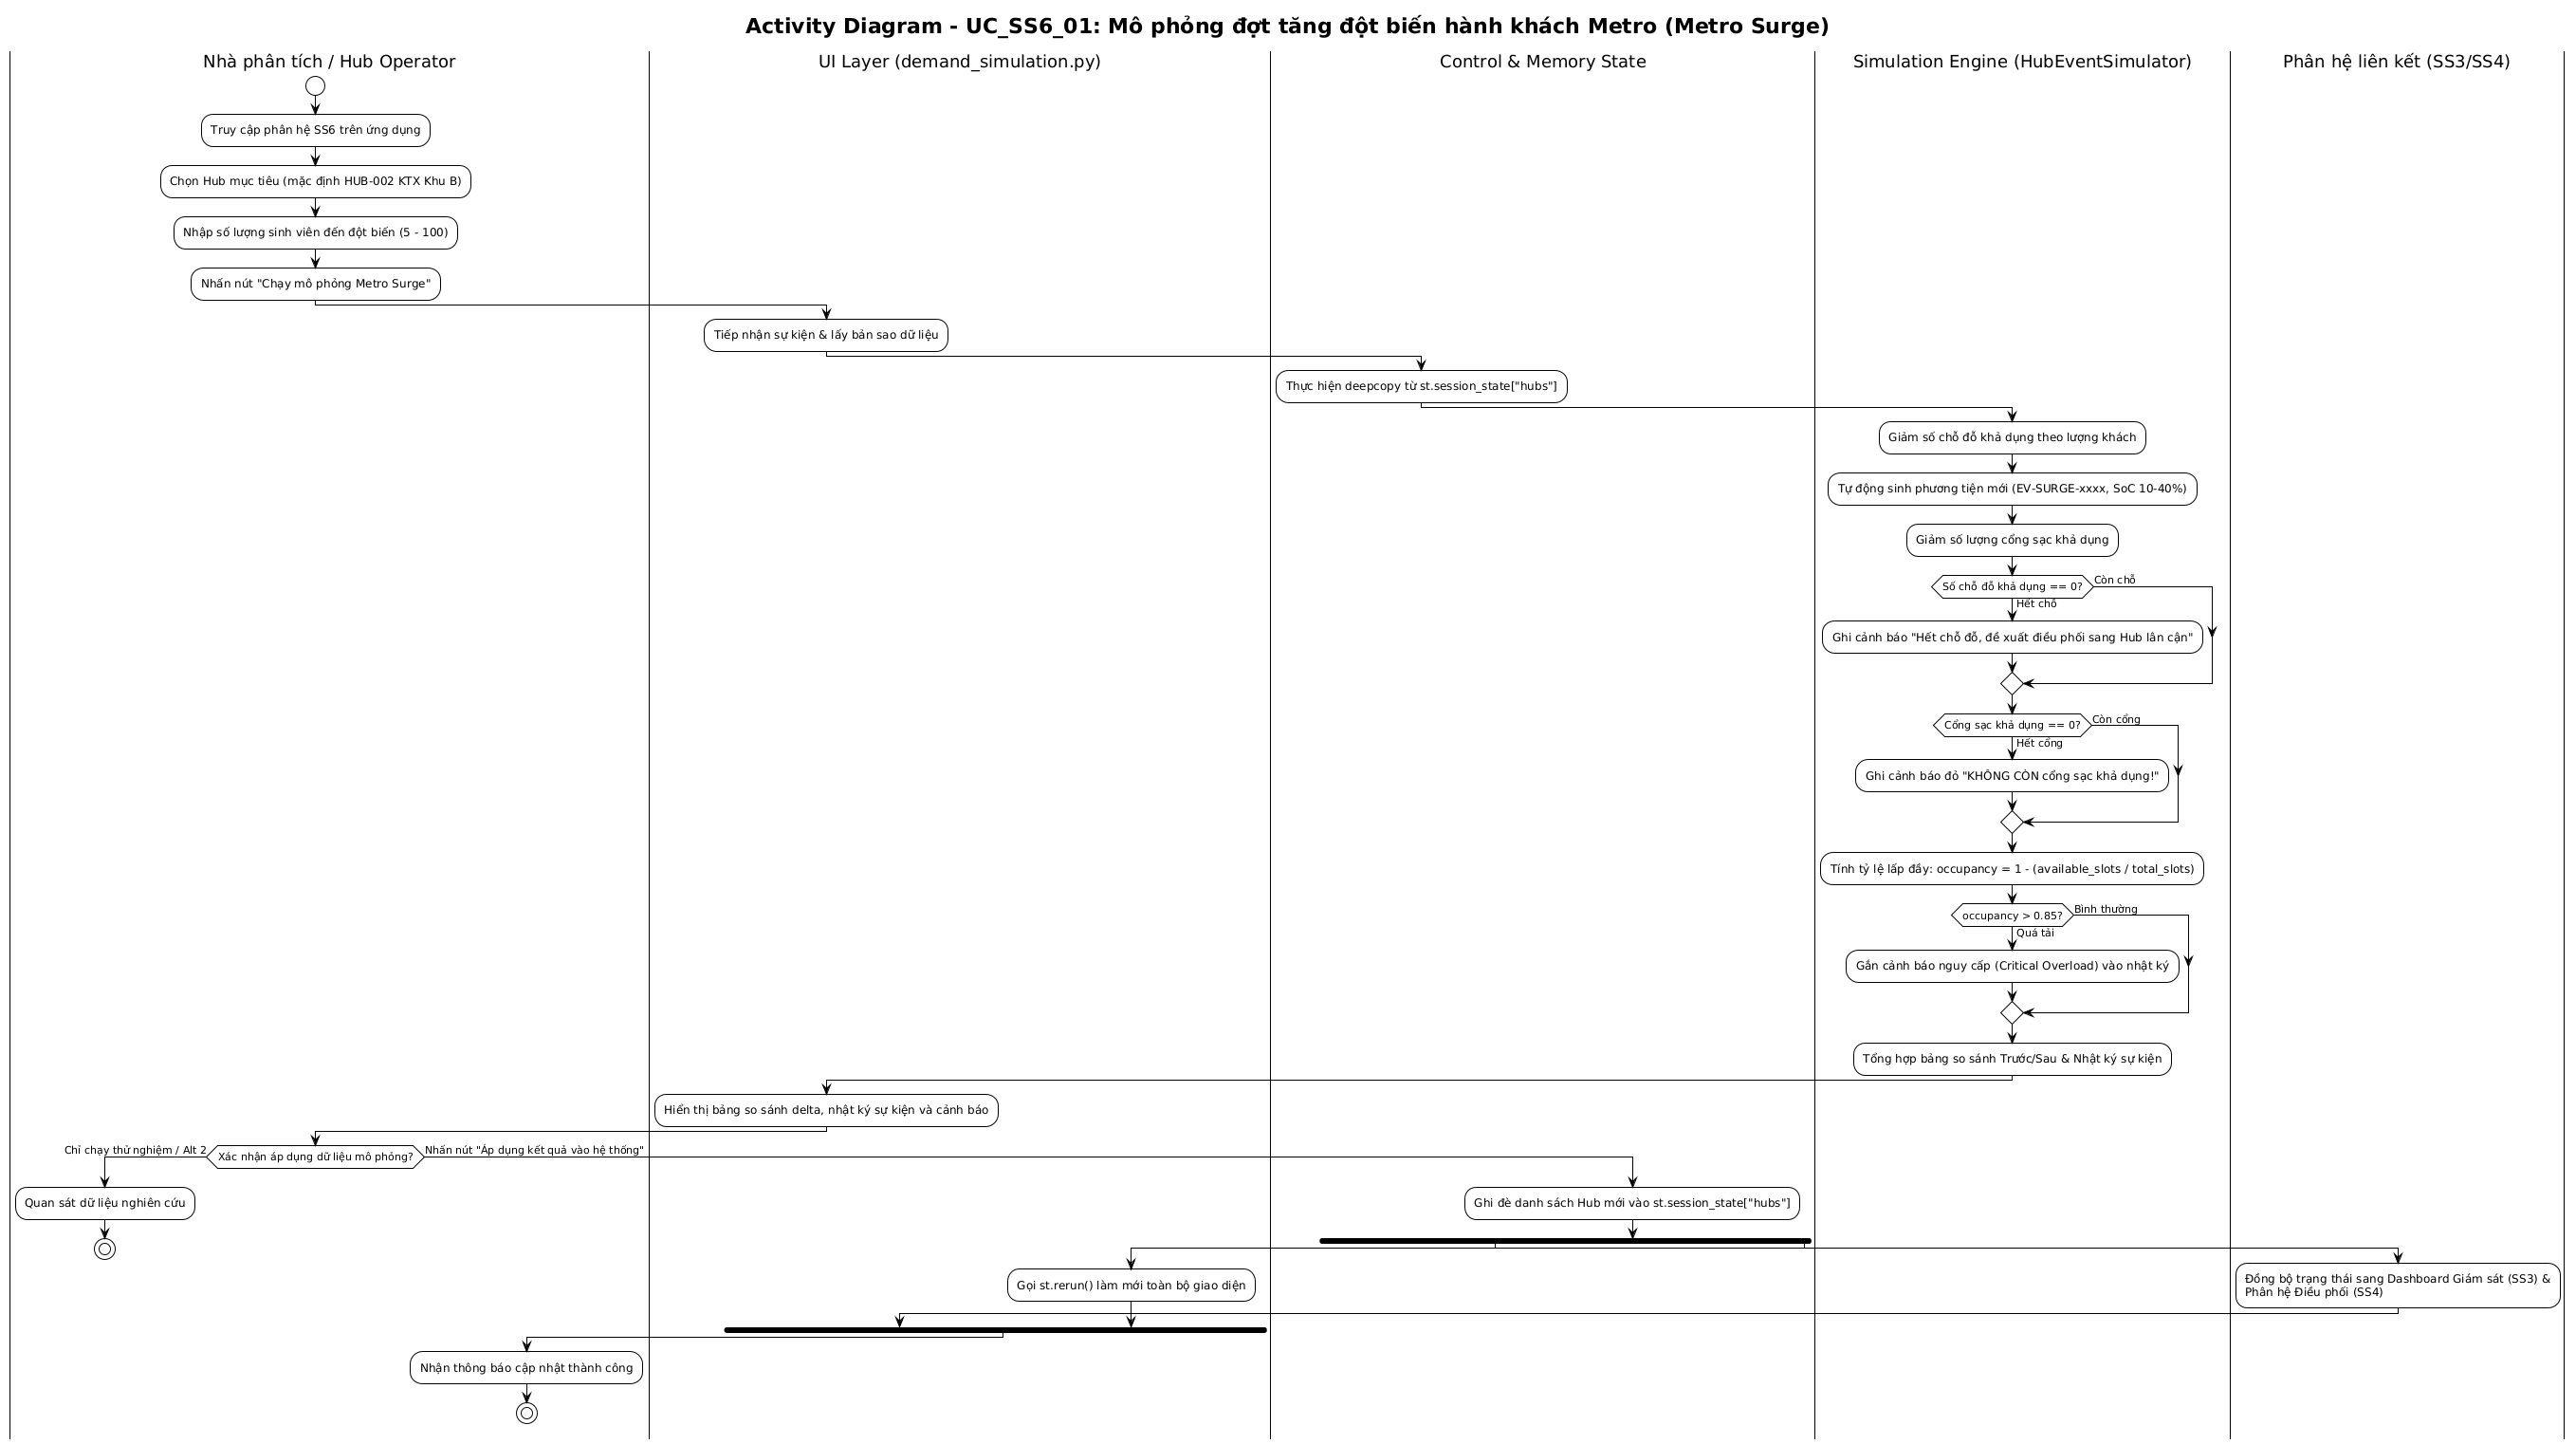
\includegraphics[width=0.92\textwidth]{Use-case detail-scenario/SS6/Activity diagrams/UC_SS6_01_HoangVanTan_activity.png}
    \caption{Sơ đồ Hoạt động Phân làn -- UC\_SS6\_01}
    \label{fig:act-ss6-01}
\end{figure}

\subsubsection{UC\_SS6\_02: Dự báo nhu cầu theo giờ \& Phân tích hàng đợi}
\begin{figure}[H]
    \centering
    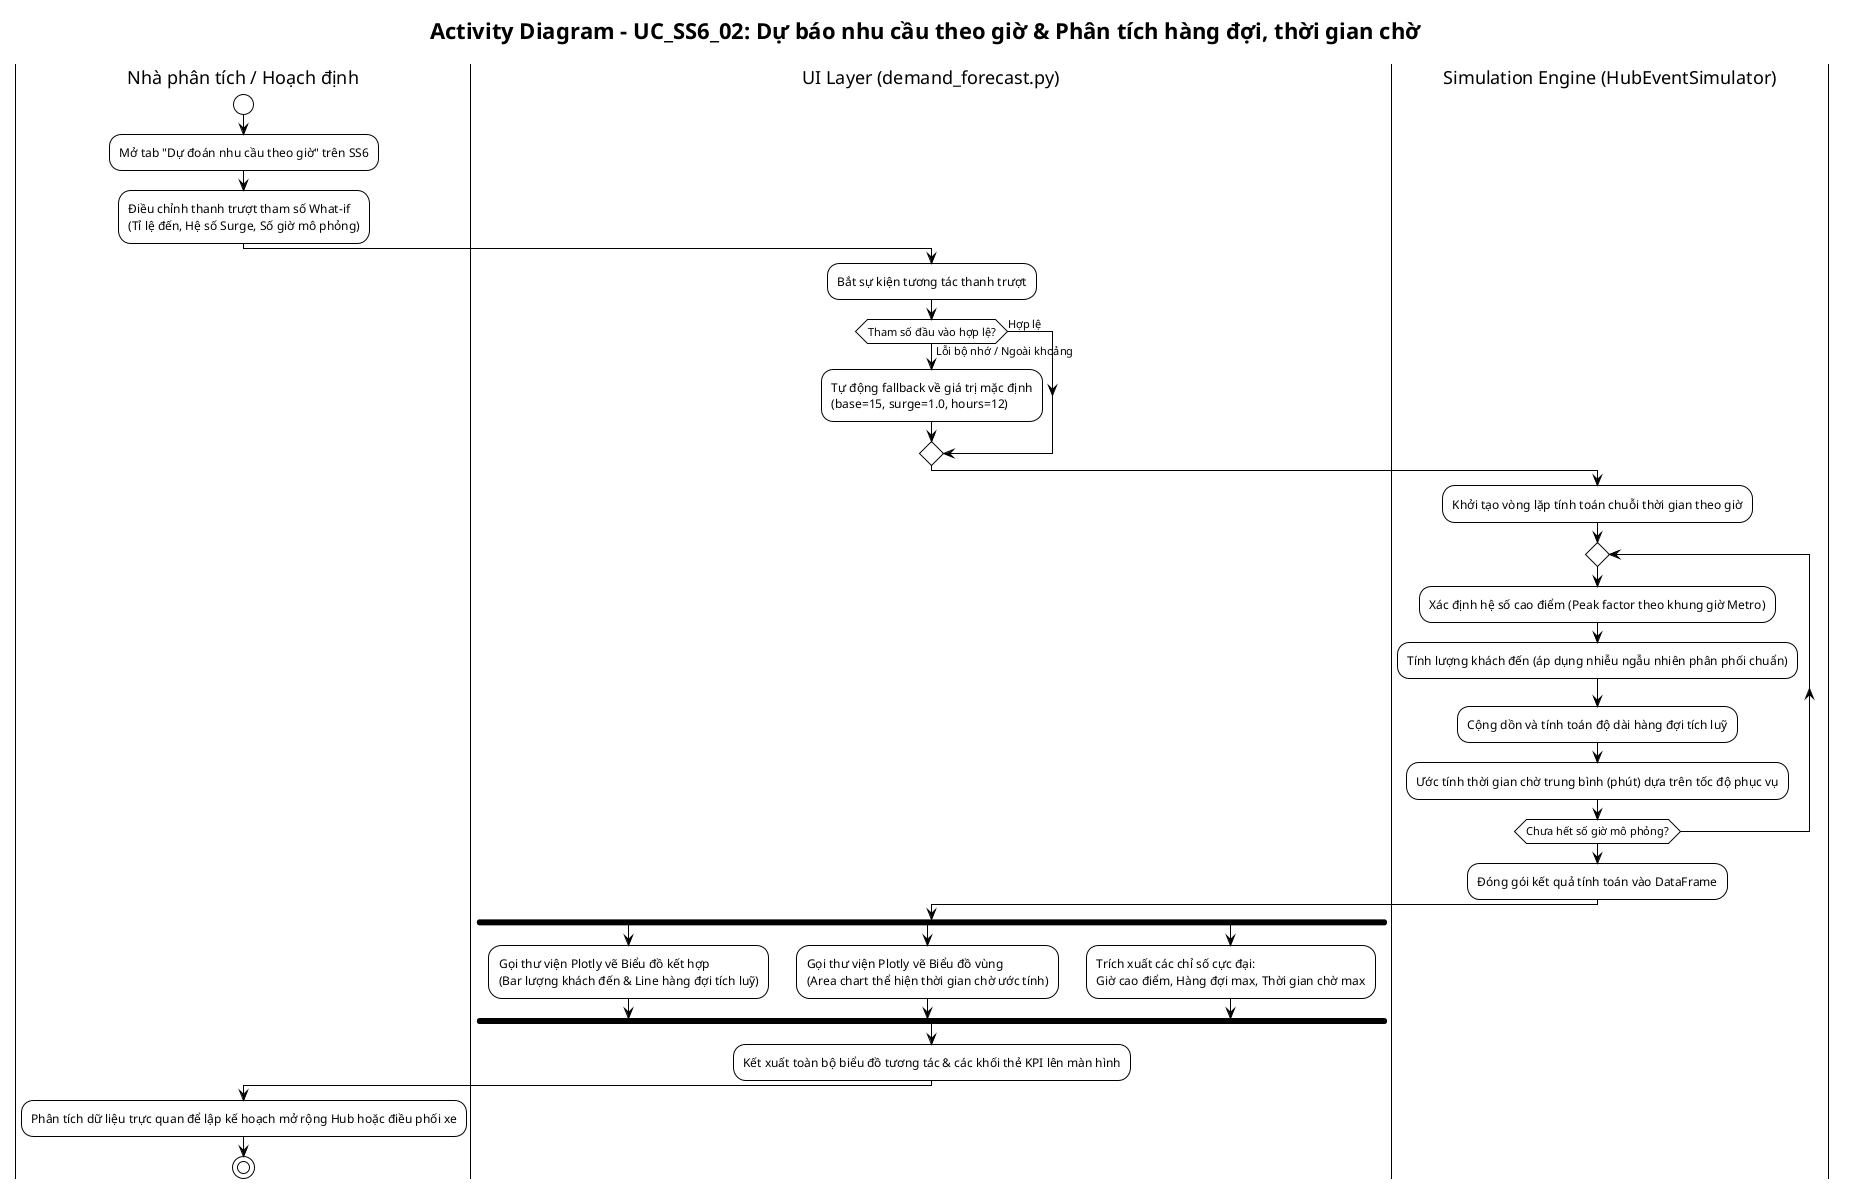
\includegraphics[width=0.92\textwidth]{Use-case detail-scenario/SS6/Activity diagrams/UC_SS6_02_HoangVanTan_activity.png}
    \caption{Sơ đồ Hoạt động Phân làn -- UC\_SS6\_02}
    \label{fig:act-ss6-02}
\end{figure}

\subsection{Phân hệ SS7: Mô phỏng What-if Hạ tầng (Nguyễn Trung Nguyên)}
\subsubsection{UC\_SS7\_01: Mô phỏng sự cố mất điện / lỗi cổng sạc}
\begin{figure}[H]
    \centering
    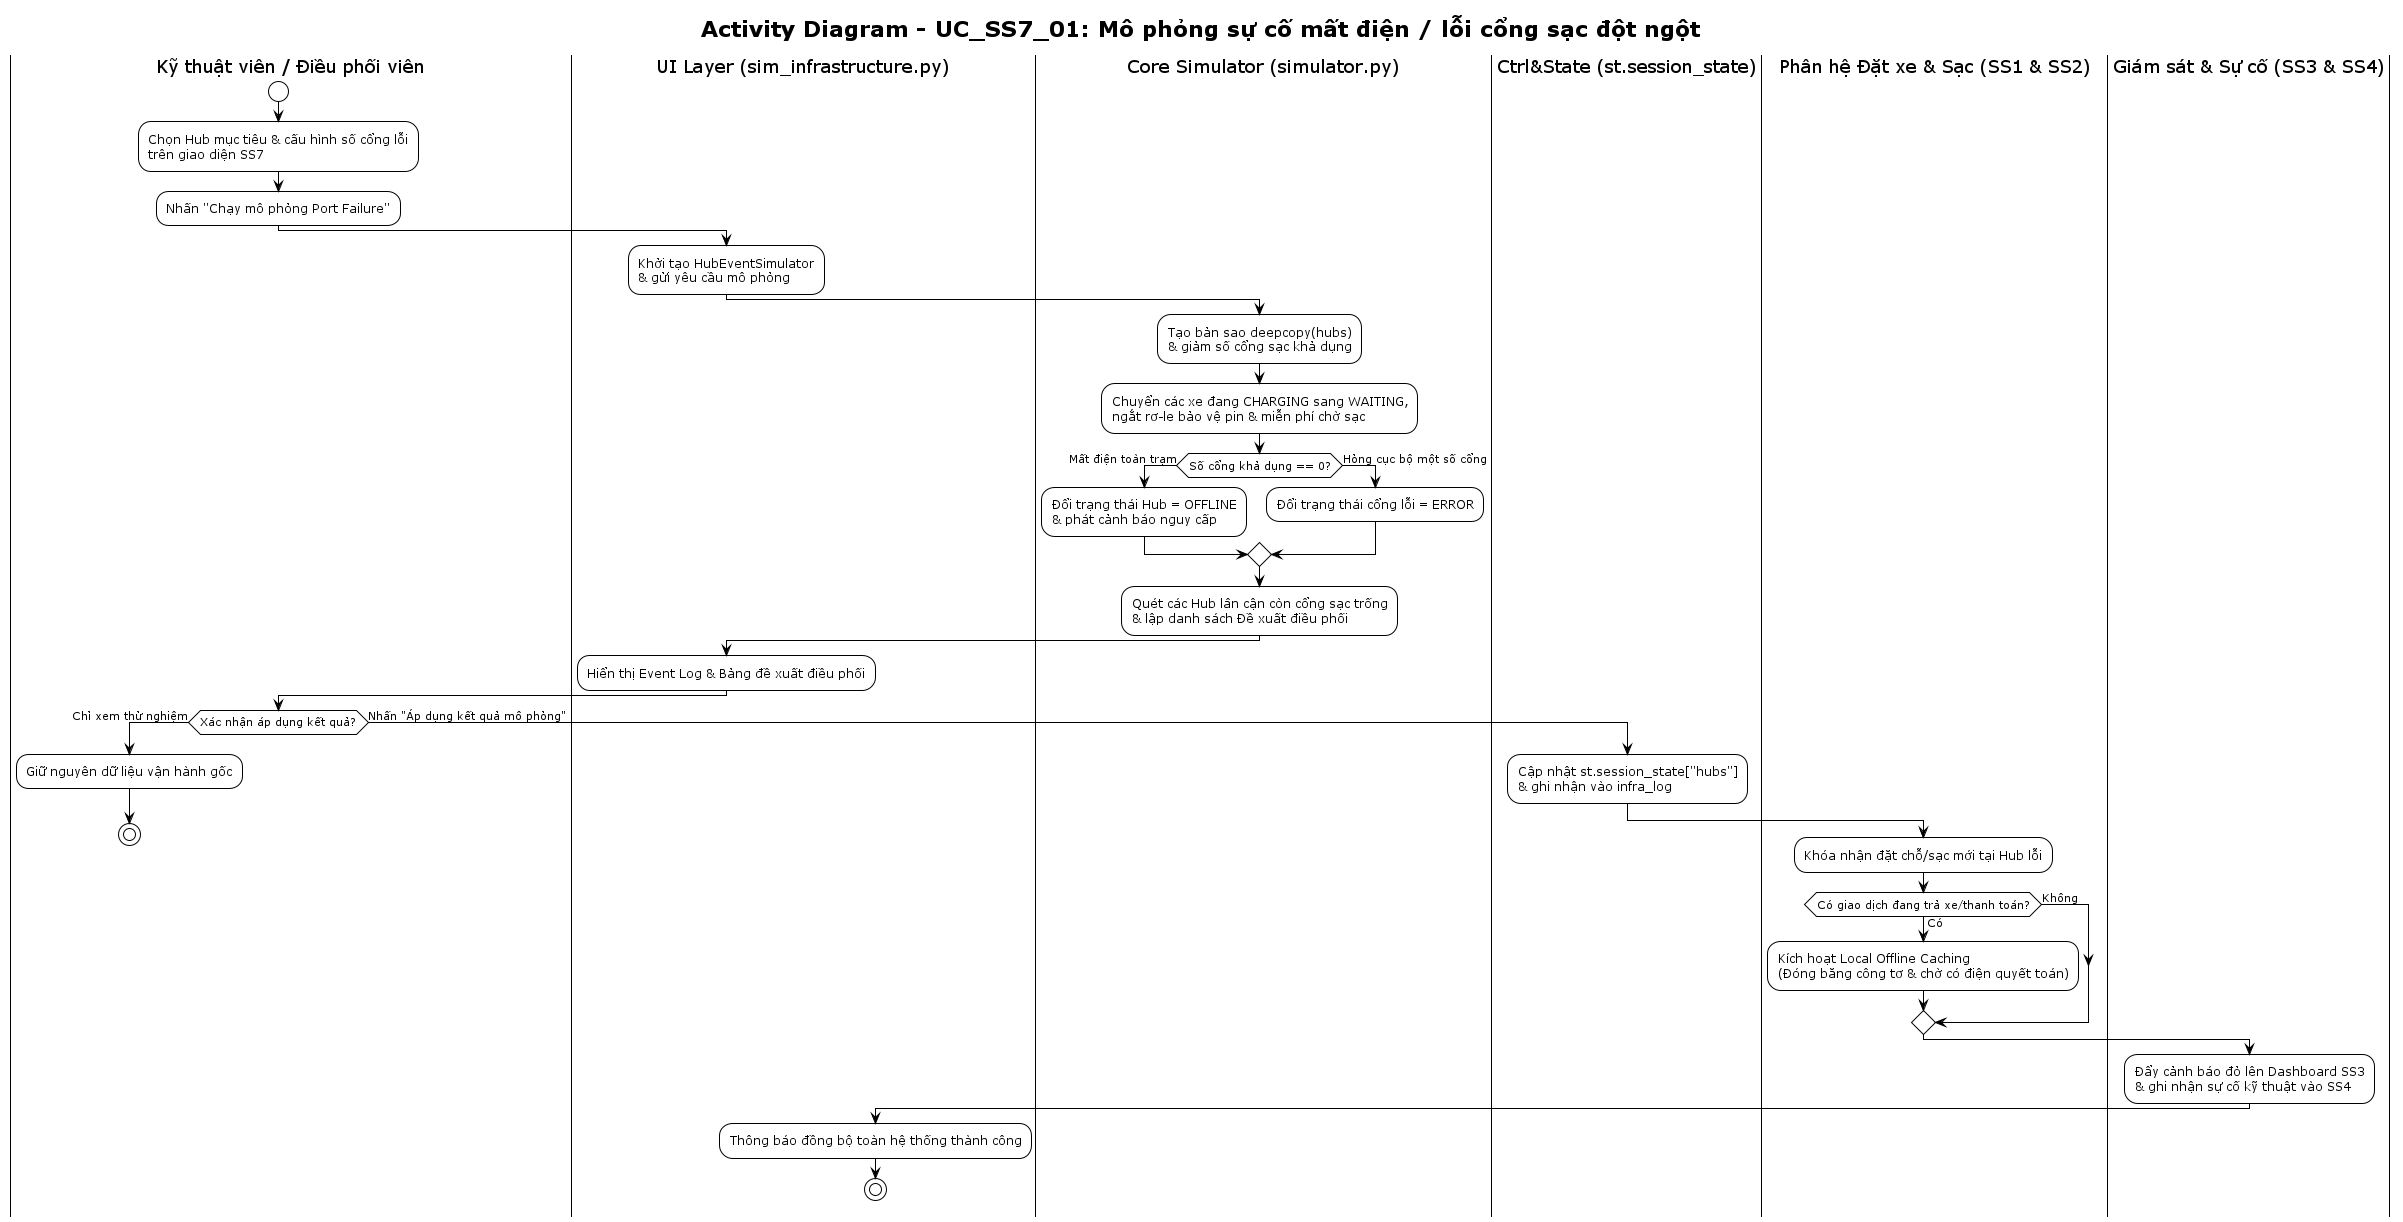
\includegraphics[width=0.92\textwidth]{Use-case detail-scenario/SS7/Activity diagrams/UC_SS7_01_NguyenTrungNguyen_activity.png}
    \caption{Sơ đồ Hoạt động Phân làn -- UC\_SS7\_01}
    \label{fig:act-ss7-01}
\end{figure}

\subsubsection{UC\_SS7\_02: Tự động phát cảnh báo \& Gợi ý điều hướng 1-chạm}
\begin{figure}[H]
    \centering
    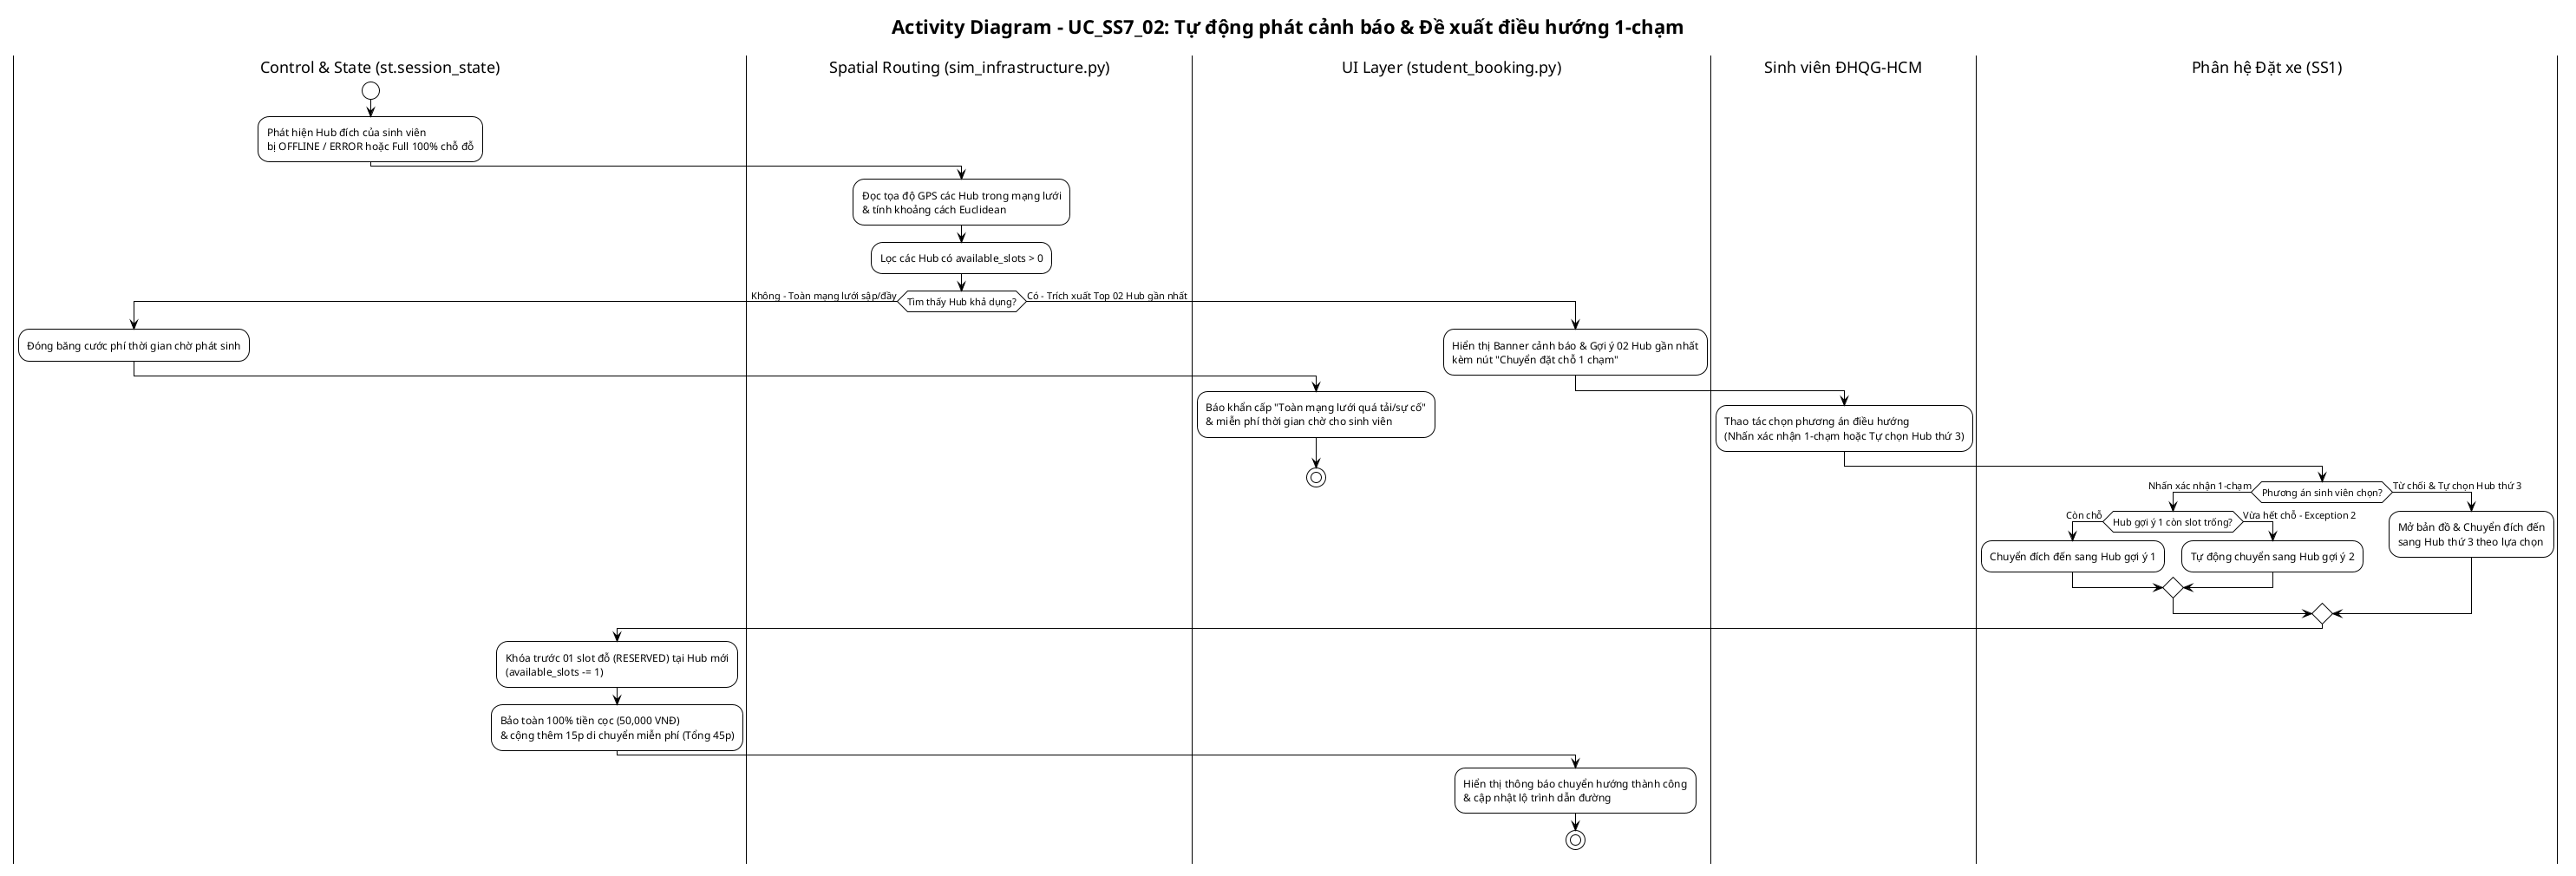
\includegraphics[width=0.92\textwidth]{Use-case detail-scenario/SS7/Activity diagrams/UC_SS7_02_NguyenTrungNguyen_activity.png}
    \caption{Sơ đồ Hoạt động Phân làn -- UC\_SS7\_02}
    \label{fig:act-ss7-02}
\end{figure}
\newpage

% ============================================================
%       MỤC 4: SƠ ĐỒ TRẠNG THÁI - STATE-CHART DIAGRAMS (BONUS)
% ============================================================
\section{Sơ đồ Trạng thái -- State-chart Diagrams (Bonus Work)}

\subsection{Vòng đời trạng thái Phương tiện \& Đặt chỗ}
Đặc tả vòng đời chuyển đổi trạng thái của phương tiện dùng chung từ khi sẵn sàng, được đặt chỗ, đang lưu thông, cho đến khi trả xe hoặc gặp sự cố:
\[
\text{AVAILABLE} \xrightarrow{\text{Đặt xe}} \text{RESERVED} \xrightarrow{\text{Mở khóa}} \text{IN\_USE} \xrightarrow{\text{Trả xe}} \text{AVAILABLE / CHARGING / INCIDENT}
\]

\begin{figure}[H]
    \centering
    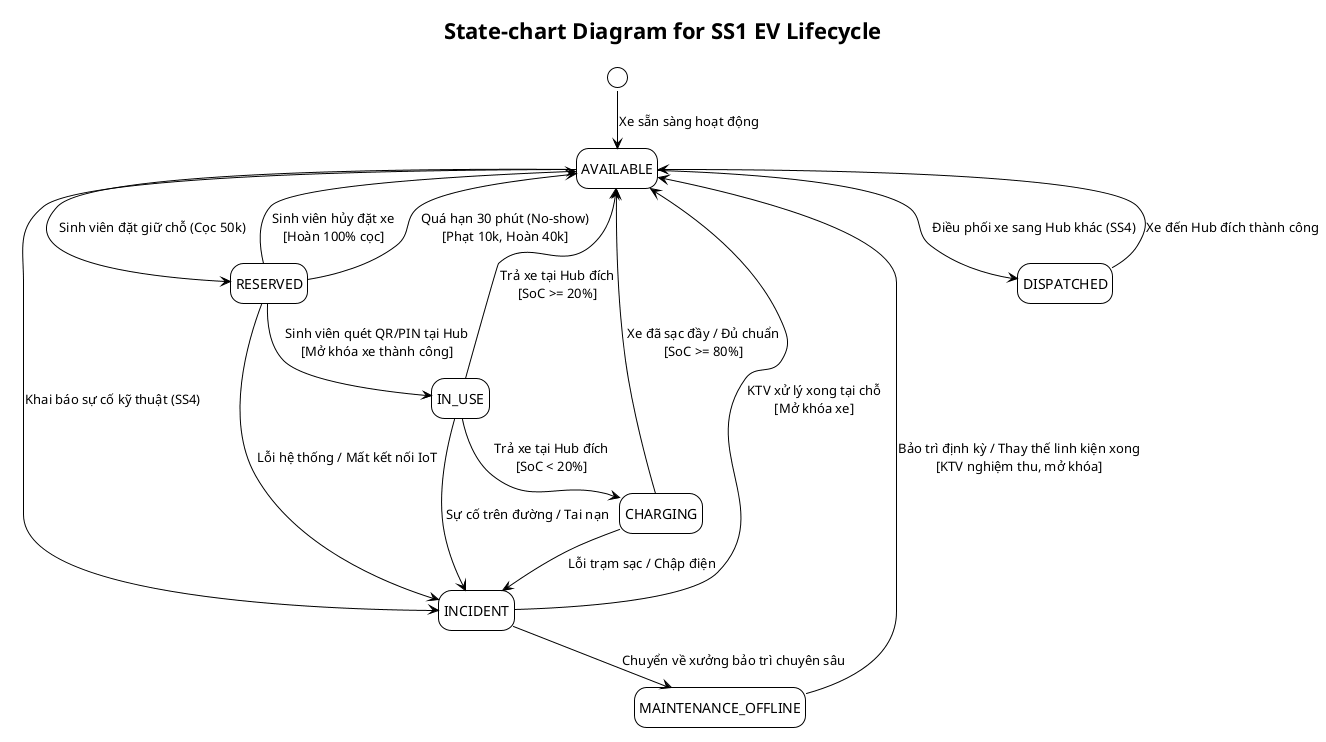
\includegraphics[width=0.92\textwidth]{Use-case detail-scenario/SS1/State-chart diagrams/UC_SS1_NguyenThanhDat_statechart.png}
    \caption{Sơ đồ Trạng thái Vòng đời Phương tiện Điện dùng chung (EV Lifecycle)}
    \label{fig:state-ev}
\end{figure}

\begin{table}[H]
    \centering
    \small
    \renewcommand{\arraystretch}{1.3}
    \caption{Bảng Đặc tả Chuyển Trạng thái Vòng đời Xe Điện}
    \label{tab:state-ev-spec}
    \begin{tabularx}{\textwidth}{|l|l|l|X|l|}
        \hline
        \textbf{Trạng thái gốc} & \textbf{Sự kiện (Event)} & \textbf{Điều kiện (Guard)} & \textbf{Hành động (Action)} & \textbf{Trạng thái đích} \\
        \hline
        AVAILABLE & Sinh viên đặt chỗ & Số dư ví $\ge 50.000$đ & Khóa cọc, sinh mã QR/PIN & RESERVED \\
        RESERVED & Quét mã QR/PIN & Mã hợp lệ, $< 15$ phút & Mở chốt điện, tính giờ & IN\_USE \\
        RESERVED & Timeout hủy & Quá 15 phút chưa nhận & Hủy đặt, hoàn 100\% cọc & AVAILABLE \\
        IN\_USE & Cắm trả tại Hub & Cổng khóa nhận diện & Tính cước, hoàn cọc thừa & AVAILABLE \\
        IN\_USE & Pin $< 20\%$ & Cắm vào cổng sạc & Chuyển sang hàng đợi sạc & CHARGING \\
        Bất kỳ & Báo cáo sự cố & KTV / SV gửi cảnh báo lỗi & Khóa xe trên hệ thống & INCIDENT \\
        \hline
    \end{tabularx}
\end{table}

\subsection{Vòng đời trạng thái Cổng sạc \& Phiên sạc (Phí chiếm dụng Overstay)}
Trụ sạc thông minh quản lý chuyển đổi giữa các trạng thái cắm sạc, đang sạc, sạc hoàn tất và trạng thái chiếm dụng trụ sạc (Overstay Fee):
\[
\text{IDLE} \rightarrow \text{PLUGGED\_IN} \rightarrow \text{CHARGING} \rightarrow \text{FULLY\_CHARGED} \xrightarrow{> 15\text{p}} \text{OVERSTAY}
\]

\begin{figure}[H]
    \centering
    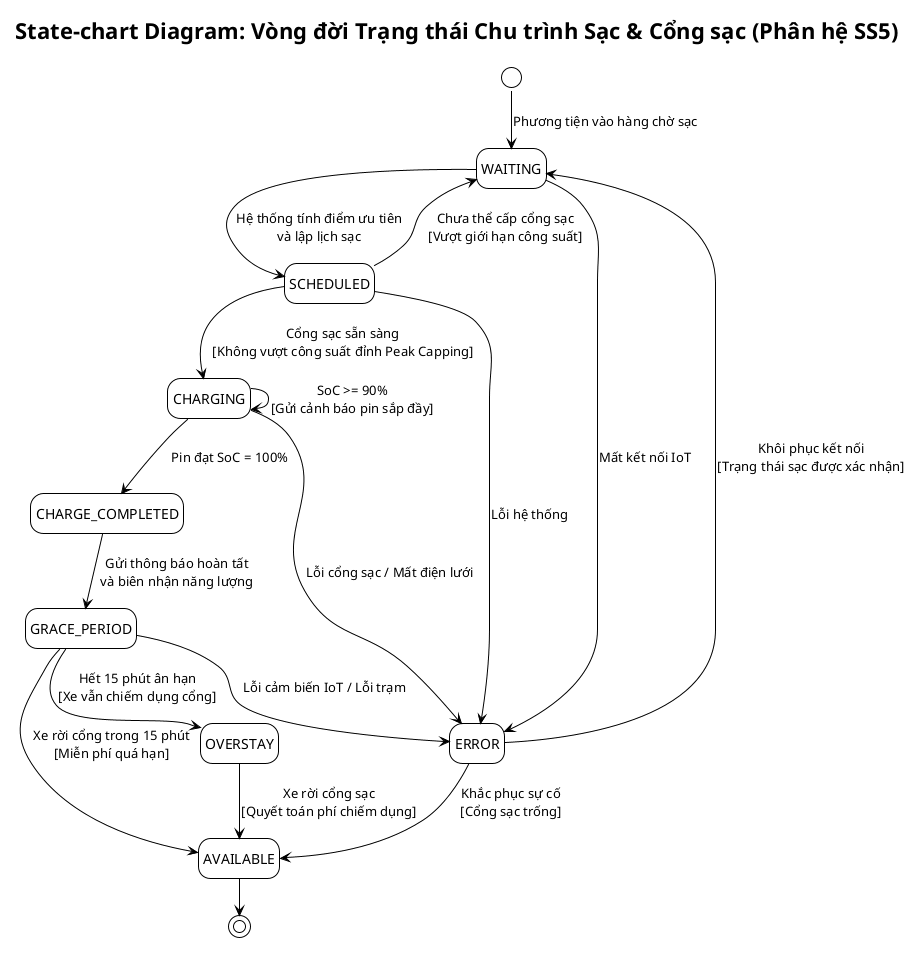
\includegraphics[width=0.92\textwidth]{Use-case detail-scenario/SS5/State-chart diagrams/UC_SS5_DuongDangKhoa_statechart.png}
    \caption{Sơ đồ Trạng thái Cổng sạc \& Phí chiếm dụng trụ sạc (Overstay Fee)}
    \label{fig:state-charging}
\end{figure}

\begin{table}[H]
    \centering
    \small
    \renewcommand{\arraystretch}{1.3}
    \caption{Bảng Đặc tả Chuyển Trạng thái Cổng Sạc \& Trụ Sạc}
    \label{tab:state-charger-spec}
    \begin{tabularx}{\textwidth}{|l|l|l|X|l|}
        \hline
        \textbf{Trạng thái gốc} & \textbf{Sự kiện (Event)} & \textbf{Điều kiện (Guard)} & \textbf{Hành động (Action)} & \textbf{Trạng thái đích} \\
        \hline
        IDLE & Cắm súng sạc & Xe kết nối hợp lệ & Kiểm tra thông tin xe & PLUGGED\_IN \\
        PLUGGED\_IN & Bắt đầu cấp điện & Đến lượt trong hàng đợi sạc & Đóng rơ-le, cấp điện áp & CHARGING \\
        CHARGING & Pin đạt 100\% & Dòng sạc $< 0.1\text{A}$ & Ngắt điện, push thông báo SV & FULLY\_CHARGED \\
        FULLY\_CHARGED & Thời gian $> 15$p & Xe chưa rút chốt sạc & Kích hoạt tính phí 10k/15p & OVERSTAY \\
        OVERSTAY / FULL & Rút súng sạc & Cảm biến ngắt kết nối & Quyết toán phí sạc + phạt & IDLE \\
        \hline
    \end{tabularx}
\end{table}

\subsection{Vòng đời trạng thái Vận hành của Mobility Hub}
Hệ thống giám sát Hub liên tục đánh giá tỷ lệ lấp đầy xe và trạng thái hạ tầng điện:

\begin{figure}[H]
    \centering
    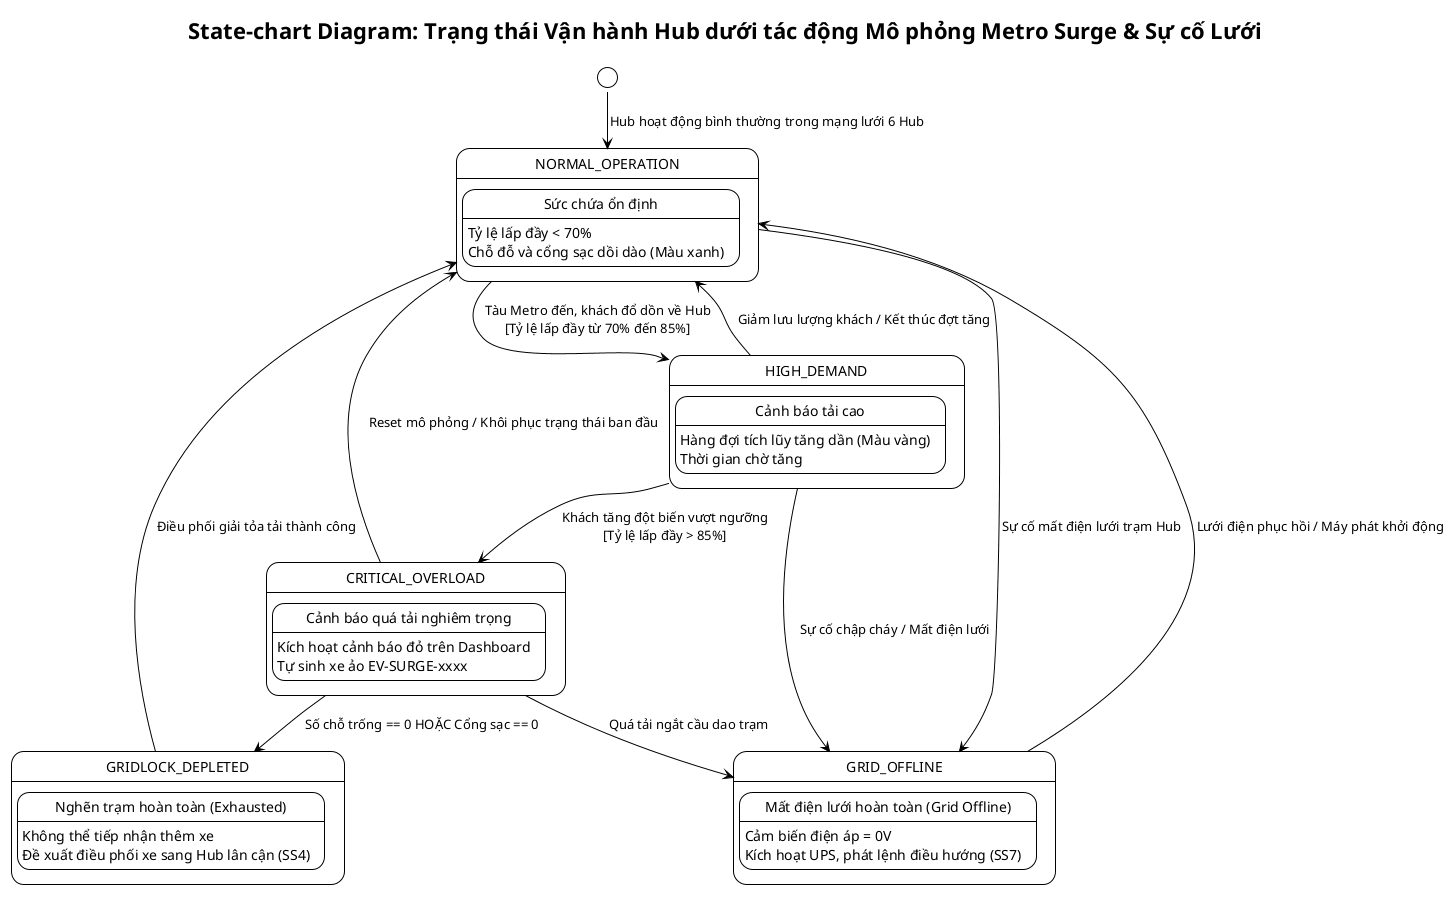
\includegraphics[width=0.92\textwidth]{Use-case detail-scenario/SS6/State-chart diagrams/UC_SS6_Hub_Operational_statechart.png}
    \caption{Sơ đồ Trạng thái Vận hành Mạng lưới Mobility Hub (Metro Surge)}
    \label{fig:state-hub}
\end{figure}

\begin{table}[H]
    \centering
    \small
    \renewcommand{\arraystretch}{1.3}
    \caption{Bảng Đặc tả Chuyển Trạng thái Vận hành Mạng lưới Mobility Hub}
    \label{tab:state-hub-spec}
    \begin{tabularx}{\textwidth}{|l|l|l|X|l|}
        \hline
        \textbf{Trạng thái gốc} & \textbf{Sự kiện (Event)} & \textbf{Điều kiện (Guard)} & \textbf{Hành động (Action)} & \textbf{Trạng thái đích} \\
        \hline
        NORMAL & Số xe tăng & $70\% \le \text{Lấp đầy} < 85\%$ & Cảnh báo Vàng trên map & ELEVATED (Vàng) \\
        ELEVATED & Số xe tiếp tục tăng & $\ge 85\%$ tải & Cảnh báo Đỏ, đề xuất điều xe SS4 & CRITICAL (Cam/Đỏ) \\
        CRITICAL & Hết sạch chỗ đỗ & Đạt $100\%$ dung lượng & Khóa nhận xe tại Hub, đổi Hub khác & EXHAUSTED \\
        Bất kỳ & Mất điện lưới & Cảm biến điện áp $= 0$ & Kích hoạt UPS, gợi ý điều hướng SS7 & GRID\_OFFLINE \\
        GRID\_OFFLINE & Điện phục hồi & Điện áp ổn định $\ge 1$ phút & Đồng bộ dữ liệu IoT, mở lại trạm & NORMAL \\
        \hline
    \end{tabularx}
\end{table}
\newpage

% ============================================================
%                       PHỤ LỤC (APPENDIX)
% ============================================================
\appendix
\section{Cấu trúc Thư mục và Mã nguồn Dự án}

\subsection{Mã nguồn Dự án (GitHub Repository)}
Mã nguồn toàn bộ hệ thống Smart E-Mobility Hub được quản lý tập trung và kiểm soát phiên bản theo chuẩn GitHub Flow tại địa chỉ chính thức:
\begin{center}
    \url{https://github.com/Dat-nguyen195/BTL_1_CNPM}
\end{center}

\subsection{Cấu trúc Thư mục Dự án (Project Directory Structure)}
Dưới đây là cây thư mục hoàn chỉnh của dự án tại mốc bàn giao \textbf{Submission \#2}, phản ánh đầy đủ việc tổ chức các sơ đồ tuần tự, hoạt động, trạng thái và giao diện người dùng:

{\footnotesize
\begin{verbatim}
smart-emobility-hub/
|-- .gitignore                     # Cấu hình bỏ qua file biên dịch, IDE và AI metadata
|-- README.md                      # Tài liệu tổng quan kiến trúc và hướng dẫn cài đặt
|-- requirements.txt               # Danh mục thư viện Python (Streamlit, Plotly, ...)
|-- docs/                          # Toàn bộ tài liệu kỹ thuật của dự án
|   |-- ai-statement.md            # Cam kết liêm chính học thuật và minh bạch AI
|   |-- tasks-assignment.md        # Ma trận phân công nhiệm vụ và tiến độ 7 thành viên
|   |-- meeting-minutes/           # Biên bản họp nhóm định kỳ (LaTeX, Markdown, PDF)
|   |-- prompt-history/            # Lịch sử câu lệnh Prompt AI của 7 thành viên
|   |-- diagrams/                  # Toàn bộ sơ đồ thiết kế hệ thống
|   |   |-- system/                # Sơ đồ Use-Case tổng thể hệ thống (smartEhub.drawio)
|   |   +-- Use-case detail-scenario/
|   |       |-- SS1/               # Phân hệ SS1 (Nguyễn Thành Đạt)
|   |       |   |-- Activity diagrams/     # UC_SS1_01..03 (.puml + .png)
|   |       |   |-- Sequence diagrams/     # UC_SS1_01..03 (.puml + .png)
|   |       |   |-- State-chart diagrams/  # EV Lifecycle (.puml + .png)
|   |       |   +-- Usecase scenario/      # Kịch bản chi tiết (.md + .docx)
|   |       |-- SS2/               # Phân hệ SS2 (Nguyễn Anh Tài)
|   |       |   |-- Activity diagrams/     # UC_SS2_01..04 (.puml + .png)
|   |       |   |-- Sequence diagrams/     # UC_SS2_01..04 (.puml + .png)
|   |       |   |-- State-chart diagrams/  # Personal EV (.puml + .png)
|   |       |   +-- Usecase scenario/      # Kịch bản chi tiết (.md + .docx)
|   |       |-- SS3/               # Phân hệ SS3 (Phạm Tiến Đạt)
|   |       |   |-- Activity diagrams/     # UC_SS3_01..02 (.puml + .png)
|   |       |   |-- Sequence diagrams/     # UC_SS3_01..02 (.puml + .png)
|   |       |   |-- State-chart diagrams/  # Hub Monitoring (.puml + .png)
|   |       |   +-- Usecase scenario/      # Kịch bản chi tiết (.md + .docx)
|   |       |-- SS4/               # Phân hệ SS4 (Đặng Hoàng Quý Nhân)
|   |       |   |-- Activity diagrams/     # UC_SS4_01..02 (.puml + .png)
|   |       |   |-- Sequence diagrams/     # UC_SS4_01..02 (.puml + .png)
|   |       |   |-- State-chart diagrams/  # Dispatch & Incident (.puml + .png)
|   |       |   +-- Usecase scenario/      # Kịch bản chi tiết (.md + .docx)
|   |       |-- SS5/               # Phân hệ SS5 (Dương Đăng Khoa)
|   |       |   |-- Activity diagrams/     # UC_SS5_01..02 (.puml + .png)
|   |       |   |-- Sequence diagrams/     # UC_SS5_01..02 (.puml + .png)
|   |       |   |-- State-chart diagrams/  # Charging Lifecycle (.puml + .png)
|   |       |   +-- Usecase scenario/      # Kịch bản chi tiết (.md + .docx)
|   |       |-- SS6/               # Phân hệ SS6 (Hoàng Văn Tấn)
|   |       |   |-- Activity diagrams/     # UC_SS6_01..02 (.puml + .png)
|   |       |   |-- Sequence diagrams/     # UC_SS6_01..02 (.puml + .png)
|   |       |   |-- State-chart diagrams/  # Metro Surge (.puml + .png)
|   |       |   +-- Usecase scenario/      # Kịch bản chi tiết (.md + .docx)
|   |       +-- SS7/               # Phân hệ SS7 (Nguyễn Trung Nguyên)
|   |           |-- Activity diagrams/     # UC_SS7_01..02 (.puml + .png)
|   |           |-- Sequence diagrams/     # UC_SS7_01..02 (.puml + .png)
|   |           |-- State-chart diagrams/  # Infrastructure (.puml + .png)
|   |           +-- Usecase scenario/      # Kịch bản chi tiết (.md + .docx)
|   +-- report/                    # Báo cáo các đợt nộp học phần CO3001
|       |-- assets/                # Logo ĐHBK và hình ảnh bìa mẫu dùng chung
|       |   +-- mau.png
|       |-- scripts/               # Scripts tự động sinh báo cáo
|       |-- submission_1/          # Báo cáo Submission #1 (Đặc tả Yêu cầu)
|       |   |-- REPORT_SUBMISSION_1.tex
|       |   +-- REPORT_SUBMISSION_1.pdf
|       +-- submission_2/          # Báo cáo Submission #2 (Thiết kế Kiến trúc & UML)
|           |-- main.tex           # File mã nguồn LaTeX chính
|           +-- REPORT_SUBMISSION_2.pdf
+-- src/                           # Mã nguồn Prototype hệ thống (Streamlit)
    |-- app.py                     # Entry point khởi chạy ứng dụng
    |-- components/                # UI components tương ứng 7 phân hệ
    |-- core/                      # Thuật toán điều phối, lập lịch và mô phỏng
    +-- data/                      # Dữ liệu mô phỏng mạng lưới Hub
\end{verbatim}
}

\end{document}
